\documentclass[letterpaper,12pt]{report}
\usepackage[top=1in,right=1in,bottom=1in,left=1.5in,nohead,nofoot]{geometry}

% PACKAGES
%**********
\usepackage{amsmath}		% AMS Math (http://www.ams.org/tex/amslatex.html)
\usepackage{amssymb}		% AMS Symbols
\usepackage{amsthm}			% AMS Theorems
\usepackage{tocloft}		% Format the Table of Contents
\usepackage{float}			% More float commands
\usepackage{sectsty}		% Format section and chapter headings
\usepackage{graphicx}		% Insert images in eps or pdf format
\usepackage{setspace}		% Line-spacing

\usepackage[utf8]{inputenc}
\usepackage{graphicx}
\usepackage{setspace}
\doublespacing
\usepackage{algorithm}
\usepackage[noend]{algpseudocode}
\usepackage{color}
\usepackage{tcolorbox}
\usepackage{amsmath}
\usepackage{float}% http://ctan.org/pkg/float
\usepackage{gensymb}
\usepackage{makeidx}  % allows for indexgeneration
\usepackage{amssymb}
\usepackage{graphicx}
\usepackage{mathrsfs}

\usepackage{mathrsfs}
\usepackage{nd3}
\usepackage{pgf}
\usepackage{multirow,array}
\usepackage{mathpartir}
\usepackage{float}
\usepackage{tikz}
\usetikzlibrary{arrows,automata,positioning,shapes.multipart}
\usepackage{stmaryrd}

%\usepackage{natbib}
\usepackage{fancyvrb}
%\usepackage{microtype}
\usepackage{alltt}
\usepackage{listings}

\newtheorem{theorem}{Theorem}[section]
\newtheorem{lemma}[theorem]{Lemma}
\newtheorem{corollary}{Corollary}[theorem]
\newtheorem{definition}{Definition}[theorem]
%\usepackage{natbib}
%\usepackage{microtype}
% Coq lstlisting
% lstlisting coq style (inspired from a file of Assia Mahboubi)
%
\definecolor{dkviolet}{rgb}{0.58,0,0.83}
\definecolor{ltblue}{rgb}{0, 0, 0.55}
\definecolor{dkgreen}{rgb}{0.0, 0.2, 0.13}
\definecolor{dkblue}{rgb}{0,0,1}
\definecolor{dkred}{rgb}{0.55,0,0}
\lstdefinelanguage{Coq}{ 
	%
	% Anything betweeen $ becomes LaTeX math mode
	mathescape=true,
	%
	% Comments may or not include Latex commands
	texcl=false, 
	%
	% Vernacular commands
	morekeywords=[1]{Function, Section, Module, End, Require, Import, Export,
		Variable, Variables, Parameter, Parameters, Axiom, Hypothesis,
		Hypotheses, Notation, Local, Tactic, Reserved, Scope, Open, Close,
		Bind, Delimit, Definition, Let, Ltac, Fixpoint, CoFixpoint, Add,
		Morphism, Relation, Implicit, Arguments, Unset, Contextual,
		Strict, Prenex, Implicits, Inductive, CoInductive, Record,
		Structure, Canonical, Coercion, Context, Class, Global, Instance,
		Program, Infix, Theorem, Lemma, Corollary, Proposition, Fact,
		Remark, Example, Proof, Goal, Save, Qed, Defined, Hint, Resolve,
		Rewrite, View, Search, Show, Print, Printing, All, Eval, Check,
		Projections, inside, outside, Def},
	%
	% Gallina
	morekeywords=[2]{forall, exists, exists2, fun, fix, cofix, struct,
		match, with, end, as, in, return, let, if, is, then, else, for, of,
		nosimpl, when},
	%
	% Sorts
	morekeywords=[3]{Type, Prop, Set, true, false, option},
	%
	% Various tactics, some are std Coq subsumed by ssr, for the manual purpose
	morekeywords=[4]{pose, set, move, case, elim, apply, clear, hnf,
		intro, intros, generalize, rename, pattern, after, destruct,
		induction, using, refine, inversion, injection, rewrite, congr,
		unlock, compute, ring, field, fourier, replace, fold, unfold,
		change, cutrewrite, simpl, have, suff, wlog, suffices, without,
		loss, nat_norm, assert, cut, trivial, revert, bool_congr, nat_congr,
		symmetry, transitivity, auto, split, left, right, autorewrite},
	%
	% Terminators
	morekeywords=[5]{by, done, exact, reflexivity, tauto, romega, omega,
		assumption, solve, contradiction, discriminate},
	%
	% Control
	morekeywords=[6]{do, last, first, try, idtac, repeat},
	%
	% Comments delimiters, we do turn this off for the manual
	morecomment=[s]{(*}{*)},
	%
	% Spaces are not displayed as a special character
	showstringspaces=false,
	%
	% String delimiters
	morestring=[b]",
	%morestring=[d]’,
	%
	% Size of tabulations
	tabsize=3,
	%
	% Enables ASCII chars 128 to 255
	extendedchars=false,
	%
	% Case sensitivity
	sensitive=true,
	%
	% Automatic breaking of long lines
	breaklines=false,
	%
	% Default style fors listings
	basicstyle=\small,
	%
	% Position of captions is bottom
	captionpos=b,
	%
	% flexible columns
	columns=[l]flexible,
	%
	% Style for (listings') identifiers
	identifierstyle={\ttfamily\color{black}},
	% Style for declaration keywords
	keywordstyle=[1]{\ttfamily\color{dkviolet}},
	% Style for gallina keywords
	keywordstyle=[2]{\ttfamily\color{dkgreen}},
	% Style for sorts keywords
	keywordstyle=[3]{\ttfamily\color{ltblue}},
	% Style for tactics keywords
	keywordstyle=[4]{\ttfamily\color{dkblue}},
	% Style for terminators keywords
	keywordstyle=[5]{\ttfamily\color{dkred}},
	%Style for iterators
	%keywordstyle=[6]{\ttfamily\color{dkpink}},
	% Style for strings
	%	stringstyle=\ttfamily,
	% Style for comments
	commentstyle={\ttfamily\color{dkgreen}},
	%
	%moredelim=**[is][\ttfamily\color{red}]{/&}{&/},
	literate=
	{\\forall}{{\color{dkgreen}{$\forall\;$}}}1
	{\\exists}{{$\exists\;$}}1
	{<-}{{$\leftarrow\;$}}1
	{=>}{{$\Rightarrow\;$}}1
	%	{==}{{\code{==}\;}}1
	{==>}{{$\Longrightarrow\;$}}1
	%    {:>}{{\code{:>}\;}}1
	{->}{{$\rightarrow\;$}}1
	{<->}{{$\leftrightarrow\;$}}1
	{<==}{{$\leq\;$}}1
	{\#}{{$^\star$}}1 
	{\\o}{{$\circ\;$}}1 
	{\@}{{$\cdot$}}1 
	{\/\\}{{$\wedge\;$}}1
	{\\\/}{{$\vee\;$}}1
	%	{++}{{\code{++}}}1
	{~}{{\ }}1
	{\@\@}{{$@$}}1
	{\\mapsto}{{$\mapsto\;$}}1
	{\\hline}{{\rule{\linewidth}{0.5pt}}}1
	%
}[keywords,comments,strings]

\lstnewenvironment{coq}{\lstset{language=Coq}}{}

% pour inliner dans le texte
\def\coqe{\lstinline[language=Coq, basicstyle=\small]}
% pour inliner dans les tableaux / displaymath...
\def\coqes{\lstinline[language=Coq, basicstyle=\scriptsize]}

%%% Local Variables: 
%%% mode: latex
%%% Local IspellDict: british
%%% TeX-master: "main.tex"
%%% End: 

%%epistemic 
%
\newcommand{\DASL}{$\mathcal{DASL}$}
\newcommand{\SFive}{$\mathcal{S}$\textit{5}}
\newcommand{\Rel}[1]{R_{#1}}
\newcommand{\Act}[1]{[ \mathit{#1} ]}
\newcommand{\ActPos}[1]{\langle \mathit{XSTIT_{#1}} \rangle}
\newcommand{\Know}{\mathbf{K}\,} 
\newcommand{\Kns}[1]{\mathbf{K}_{\mathbf{#1}}\,} 
\newcommand{\Bel}{\mathbf{B}\,} 
\newcommand{\Bels}[1]{\mathbf{B}_{\mathbf{#1}}\,} 
\newcommand{\Pos}  {\langle \mathbf{K} \rangle\,} 
\newcommand{\Poss}[1]  {\langle \mathbf{K}_{#1} \rangle\,}
\newcommand{\BPos} {\langle \mathbf{B} \rangle\,}
\newcommand{\BPoss}[1]{\langle \mathbf{B}_{#1} \rangle\,}
\newcommand{\STIT}[1] {\mathbf{[XSTIT\ {#1}]}}
\newcommand{\Safe} {\mathbf{S}}
\newcommand{\safe} {\mathit{safe}}
\newcommand{\choice}[1]{\mathit{Choice_{#1}}}
\newcommand{\neXt}{\mathit{X}}
\newcommand{\Pal}[1]{\mathbf{[#1]}_i}
\newcommand{\PalPos}[1]{\mathbf{\langle#1\rangle}_i}
\newcommand{\SPal}[1]{\mathbf{[#1]_{\mathit{i}}^\mathcal{S}}}
%	\stackrel{\mathbf{safe}}{\mathbf{[#1,#2]}}}
\newcommand{\SPalPos}[1]{\mathbf{\langle#1\rangle_{\mathit{i}}^\mathcal{S}}}

\def\firstcircle{(90:1.75cm) circle (2.5cm)}
\def\secondcircle{(210:1.75cm) circle (2.5cm)}
\def\thirdcircle{(330:1.75cm) circle (2.5cm)}

%%qed
%
\newcommand{\qqed}{\hfill\mbox{$\Box$}}
%
%%BNF
\newcommand{\bnf}{\ |\ }
\newcommand{\indy}{\mathop{\parallel}}
\newcommand{\mmid}{\mathrel{\mid}}
%
\newcommand{\etal}{\textit{et.~al.}}
\newcommand{\nnot}{\textsf{\ not \ }}
\newcommand{\oor}{\textsf{\  or \ }}
\newcommand{\iiff}{{\  \Leftrightarrow \ }}
\newcommand {\aand}{ \textsf{\ and \ } }
\newcommand {\timplies} { \textsf{\ implies \ }}
\newcommand {\tland}{{\ \wedge \ }}
\newcommand {\tlor}{{\ \vee \ }}
\newcommand {\tlnot}{{\neg}}
\newcommand {\iimplies}{{\ \Rightarrow \ }}
%
% Algorithm style
\makeatletter
\def\BState{\State\hskip-\ALG@thistlm}
\makeatother
%
%<<<<<<\newtheorem*{exam}{Example}
%<<<<<< \newtheorem*{countex}{Counterexample}
%
%\\
%\spnewtheorem{axiom}{Axiom}{\bfseries}{\itshape} 
%\spnewtheorem{dfn}{Definition}{\bfseries}{\itshape}
%\spnewtheorem*{rmk}{Remark}{\bfseries}{\itshape}
%\spnewtheorem*{exam}{Example}{\bfseries}{\rmfamily}
%\spnewtheorem*{countex}{Counterexample}{\bfseries}{\rmfamily}
\newcommand{\li}{\mathit{i}}
\newcommand{\pre}{\mathit{pre}}
\newcommand{\lpp} {\mathit{p}}
\newcommand{\lAA}{\mathit{A}}
\newcommand{\lff} {\mathit{f}}
\newcommand{\lhh} {\mathit{h}}
\newcommand{\lhhp} {\mathit{h'}}
\newcommand{\lqq} {\mathit{q}}
\newcommand{\laa} {\mathit{a}}
\newcommand{\lbb} {\mathit{b}}
\newcommand{\ldd} {\mathit{\delta}}
\newcommand{\lnn} {\mathit{n}}
\newcommand{\luu} {\mathit{u}} 
\newcommand{\lvv} {\mathit{v}} 
\newcommand{\ltt}  {\mathit{t}} 
\newcommand{\lww} {\mathit{w}}
\newcommand{\lWW} {\mathit{W}}
\newcommand{\lMM} {\mathit{M}}
\newcommand{\lVV} {\mathit{V}}
\newcommand{\lSS} {\mathit{S}}
\newcommand{\lss} {\mathit{s}}
\newcommand{\lssp} {\mathit{s'}}
\newcommand{\lHH} {\mathit{H}}
\newcommand{\false} {\mathit{False}}
\newcommand{\true} {\mathit{True}}
\newcommand{\lyy} {\mathit{y}}
\newcommand{\lxx} {\mathit{x}}
\newcommand{\lzz}{\mathit{z}}
%
\newcommand{\bF}{\mathbb{F}}
\newcommand{\bR}{\mathbb{R}}
\newcommand{\bZ}{\mathbb{Z}}
\newcommand{\bN}{\mathbb{N}}
\newcommand{\bQ}{\mathbb{Q}}
%
% Potentially useful packages:
% \usepackage{epsfig}			% For EPS figures
% \usepackage{subfigure}		% For side-by-side figures
% \usepackage{sidecap}		% Put captions on the side of figures
% \usepackage{rotating}		% Rotatiion of figures and tables
% \usepackage{multirow}		% Column and row spanning in tables
% \usepackage{chapterbib}		% Insert bibliograhpy with a simple include command

\input{Command_Mods}	% Lots of special formatting to make the ToC adhere to MU requirements

\begin{document}

\doublespacing % Double line-spacing ( or specify something like \setspacing{1.8} )
\allsectionsfont{\singlespacing} % Only body text needs double spacing, titles can be single spaced

\setcounter{page}{1}    
\pagenumbering{roman}

\thispagestyle{empty}

\vspace*{\fill}
\centerline{\large{\bf FORMAL METHODS WITH}} % The title on the Title Page must be in all caps.
\centerline{\large{\bf DYNAMIC AGENT SAFETY LOGIC}}
\vskip 10mm
\centerline{\rule{150mm}{0.2mm}} % You can adjust the length of the horizontal line here.
\vskip 10mm
\centerline{A Thesis presented to} % Choose Thesis or Dissertation
\centerline{the Faculty of the Graduate School}
\centerline{at the University of Missouri}
\vskip 10mm
\centerline{\rule{150mm}{0.2mm}}
\vskip 10mm
\centerline{In Partial Fulfillment}
\centerline{of the Requirements for the Degree}
\centerline{Doctor of Philosophy} % Change to your degree
\vskip 10mm
\centerline{\rule{150mm}{0.2mm}}
\vskip 10mm
\centerline{by}
\centerline{Seth Ahrenbach} % Your name on the Title Page must be in all caps.
\centerline{Dr. Rohit Chadha, Thesis Supervisor} % Edit advisor and choose Thesis or Dissertation
\centerline{MAY 2005} % The month is required to be capitalized.  Use the month and year of your graduation, not the month and year you defend.
\vspace*{\fill}
	% Input the Title Page (no page number, but counts as roman numeral 'i')
\newpage
\thispagestyle{empty}

The undersigned, appointed by the Dean of the Graduate School, have 
examined the dissertation entitled: % Choose thesis or dissertation

\vspace{8mm}
\centerline{FORMAL METHODS WITH} % The title on the Title Page must be in all caps.
\centerline{DYNAMIC AGENT SAFETY LOGIC}
\vspace{8mm}
\noindent presented by Seth Ahrenbach, % Edit with your name (does not need to be in all caps.)

\noindent a candidate for the degree of Doctor of Philosophy % Change to your degree
and hereby certify that, in their opinion, it is worthy of acceptance.
\vskip 15mm
\centerline{\rule{100mm}{0.2mm}}
\centerline{Dr. Rohit Chadha} % Edit advisor
\vskip 10mm
\centerline{\rule{100mm}{0.2mm}}
\centerline{Dr. Guilherme DeSouza} % Edit committee member 1
\vskip 10mm
\centerline{\rule{100mm}{0.2mm}}
\centerline{Dr. Alwyn Goodloe} % Edit committee member 1
\vskip 10mm
\centerline{\rule{100mm}{0.2mm}}
\centerline{Dr. William Harrison} % Edit committee member 1
\vskip 10mm
\centerline{\rule{100mm}{0.2mm}}
\centerline{Dr. Paul Weirich} % Edit committee member 1
	% Input the Approval Page (no page number)
\newpage
\pagenumbering{roman}
\setcounter{page}{2}
\addcontentsline{toc}{chapter}{ACKNOWLEDGMENTS} % This is the American english spelling (no E between G and M)

\centerline{\bf \large ACKNOWLEDGMENTS}
\vskip 10mm % Edit everything below with your acknowledging text.
Without the support and encouragement of many people, I would not have produced this work. So you can blame them for any mistakes.

Producing this thesis spanned about three years, during which time I started working full time as a software developer, moved twice, and had a wonderful daughter. Without my wife's love, support, and encouragement, I would have given up. Maggie was always there to center me and help nudge me along, and I am grateful to have her in my life. I wanted to accomplish something difficult in order to set a positive example for our daughter, Ellie. I am convinced Ellie wanted this, too. She had no control over whether I would accomplish it, but she could certainly make it more difficult! She made sure it was a very positive example that I set. Much of Chapters Three and Five benefited from her very vocal criticism, and I dedicate them to her.

This particular journey began in the philosophy classroom, where I learned about modal logic from Zac Ernst. I had enjoyed the formalisms of proofs since learning geometry in middle school, and my interest in propositional and predicate logic was similarly high, but modal logic, with its weird possible worlds semantics, delivered by an engaging instructor like Zac, lit a spark in me. Paul Weirich introduced me to game theory, also from the philosophy classroom, and there may be no better instructor of what it is to be a rational agent. I sometimes wonder if he isn't the ideally rational agent that economists speak of. I later swapped Zac and Paul and had Zac teach me decision theory and Paul teach me more modal logic. I am one of the luckiest students to have benefited from both of their mentorship in these areas. After reading this thesis, you might wonder how I didn't turn out better, and you'd be right to so wonder.

Other professors in the University of Missouri Philosophy Department introduced me to subjects that I devoured and regurgitated in the present thesis, including Peter Markie's expert and truly world class instruction on epistemology. I must say that any mistake in this thesis concerning epistemology is my own, and he is blameless. I like to think that in a nearby possible world, I my counterpart continued to study epistemology under Peter Markie's counterpart. And in that possible world, Academia is a valued and respected institution, with rich and ample state support. Perhaps it is not so nearby. In any case, I sometimes envy my counterpart there, learning from one of our generation's best analytic epistemologists.

But I do not envy him so much as to risk wishing for a swap. In this world I have my wife and daughter, and Zac Ernst convinced me that it is possible to focus on modal logic as a PhD thesis, but that doing so requires a transfer to the computer science department. A mentor trifecta swirled around me there, with Bill Harrison, Rohit Chadha, and Alwyn Goodloe teaching me the difference between philosophy and computer science. Without all three of these researchers taking a chance on me, I would not have finished.

Bill took a chance on me by accepting me as a graduate student and forcing open whatever bureaucratic doors threatened to close on me, and I am grateful to him for this. Alwyn selected a mostly-philosophy grad student for a NASA aerospace engineering internship, and Rohit agreed to let me pursue the topics developed in that internship as dissertation. I am sincerely grateful for their support as I struggled to steer my mental ship from a philosophy heading to a computer science heading.	% Input the Acknowledgement Page (roman numeral page number 'ii')
\input{Contents}	% Generate and input a Table of Contents and List of Figures/Tables/etc.(roman numeral page number 'iii')

\newpage
\addcontentsline{toc}{chapter}{ABSTRACT}

\centerline{\bf \large ABSTRACT}
\vskip 10mm % Edit everything below with your acknowledging text.
Modal logic is a family of logics for reasoning about relational structures, broadly construed. It sits at the nexus of philosophy, mathematics, software engineering, and economics. By modeling a target domain as a relational structure, one can define a modal logic for reasoning about its properties. Common examples include modal logics for knowledge, belief, time, program execution, mathematical provability, and ethics. 

This thesis presents a modal logic that combines several modalities in order to reason about realistic human-like agents. We combine knowledge, belief, action, and \emph{safe} action, which we call Dynamic Agent Safety Logic, or \DASL. We distinguish \DASL\ from other modal logics treating similar topics by arguing that the standard models of human agency are not adequate. We present some criteria a logic of agency should strive to achieve, and then compare how related logics fare.

We use the Coq interactive theorem prover to mechanically prove soundness and completeness results for the logic, as well as apply it to case studies in the domain of aviation safety, demonstrating its ability to model realistic, minimally rational agents.

Finally, we examine the consequences of modeling agents capable of a certain sort of self-reflection. Such agents face a formal difficulty due to L\"ob's Theorem, called L\"ob's Obstacle in the literature. We show how \DASL\ can be relaxed to avoid L\"ob's Obstacle, while the other modal logics of agency cannot easily do so.

\newpage
\setcounter{page}{1}
\pagenumbering{arabic}
\addtocontents{toc}{\protect \contentsline {chapter}{CHAPTER}{}}

\chapter{Introduction}
	\label{CH_Intro}

In this doctoral thesis, I present a logic for reasoning about safety-critical information flow among machines and humans. The thesis advances the domain of modal logic by developing a rich and expressive logic suitable for reasoning about real humans in real situations, which in turn provides a new tool for formal methods researchers interested in developing safe human-machine hybrid systems. Thus, the thesis is interdisciplinary, pulling from fields as diverse as philosophy, game theory, computer science, and safety engineering.  
%
%My work intersects with logic, game theory, information assurance, and aviation safety. I address a problem confronting formal methods researchers in that the vast majority of the methods used to verify system safety and security fail to address the human component. In both aviation safety, and more generally in complex systems, system failure often involves human behavior playing a critical role. I solve this problem by providing a mathematically precise logic for reasoning about the relationship between agents' actions and the safety-critical information they are aware of.

The logic, which I call Dynamic Agent Safety Logic (DASL), is based on the logical foundations of game theory, in which models of agency formally capture how knowledge, rationality, and action relate to each other. Game theory presents a model that, given a description of a scenario, allows one to deduce what actions are dictated by a given theory of rationality. The standard game-theoretic inference works as follows:
\begin{equation*}
\mathit{Knowledge\_of\_Situation} \tland \mathit{Rationality} \iimplies \mathit{Good\_Action}.
\end{equation*}
One can read this as, ``if an agent has knowledge of a situation (\emph{e.g.} a game), and the agent is rational, then the agent executes a good action. In game theory, the important terms are suitably formalized for mathematical treatment. Knowledge is assumed to be perfect, rationality is defined as the maximization of some measure of utility, and good actions are those that bring about the outcomes with the most possible utility payoffs. The definitions make the inference an analytic truth.

Empirically, however, humans frequently deviate from the prescribed behavior. Looking at the above formula, we can ask a question: what can we infer when an agent fails to execute the prescribed action, as when pilots provide unsafe control inputs to their aircrafts? We can answer this question by examining the contrapositive of the above game-theoretic inference:
\begin{equation*}
\tlnot \mathit{Good\_Action} \iimplies \tlnot (\mathit{Knowledge\_of\_Situation} \tland \mathit{Rationality}),
\end{equation*}
or equivalently,
\begin{equation*}
\tlnot \mathit{Good\_Action} \iimplies \tlnot \mathit{Knowledge\_of\_Situation} \tlor \tlnot \mathit{Rationality}.
\end{equation*}
 
With a bit more Boolean manipulation, we have the following:
\begin{equation*}
\tlnot \mathit{Good\_Action} \tland \mathit{Rationality} \iimplies \tlnot \mathit{Knowledge\_of\_Situation}.
\end{equation*}
This can be read, ``If an agent is rational but executes a bad action, then the agent lacked knowledge of the situation." Thus, embedded in the classical game-theoretic model of agency is a logical inference from bad action to missing knowledge. This makes intuitive sense upon reflection. If someone is rational, yet they commit an irrational (read: ``bad") action, then it must be the case that they didn't know some crucial information. With this insight in hand, I identify a logic in which the above inference is sound, with details about which particular pieces of information are missing from an agent's knowledge base when she executes a bad action. Again, it should not be surprising that such a logic exists, because classical game theory already posits a \emph{logical} relationship between knowledge of particular propositions and particular actions.

I have formally captured such inferences with DASL, where a rational agent executes a bad action, and from this we can infer which safety-critical information they are missing. This can be done at run-time, as demonstrated herein by a prototype that uses the Z3 theorem prover to compute relevant part of the inference, formalized as a set of clauses in first order logic. The prototype satisfies an information assurance property not yet treated formally by the literature, but done so here with DASL. The property formalizes the idea that safety-critical information should not fail to reach a human and inform her actions. This is more than the information assurance property of \emph{availability}, because it is available to her only in a passive sense. It must be actively and specifically \emph{delivered} by ensuring that non-critical information does not compete for the human's awareness at critical moments. Formally specifying this property is another contribution of this thesis. 

I apply these formal ideas to the domain of aviation safety, specifically incidents involving pilot errors that contribute to fatal mishaps. This is both an important area of research, where advancements can help save lives, but it also satisfies some desirable properties as a domain. When a new modal logic is developed, it is usually first applied to simple, closed domains, like games, involving simple agents with relatively few choices compared to the rich variability one can find in real life. Similarly, the environmental factors modeled in these situations are usually quite closed. To extend these logics into a realistic domain involving complex human agents and environments is quite a leap. The cockpit is a nice step between the two, because the relevant environment is not simple, but not as rich as a more general environment. The environment that must be modeled consists of discrete instruments with a somewhat limited range of possible values. The agents are real humans, but concerned with a limited number of actions involving inputs that manipulate the airplane's flight. Another advantage of the human agents in aviation is that they are highly trained, and so meet a level of rationality in the problem space that is not quite the full blown rationality of game theoretic agents, but is certainly better than an average human navigating a random problem encountered in the real world. Thus, human pilots in the cockpit are a Goldilocks zone of human agency that is more realistic than the agents in most game examples, but not quite as complex as humans in the more general problem space of reality writ large.

By developing a logic that can model the information flow in these situations, we advance the project of formally reasoning about human agency. Credit for initiating this project belongs to many researchers over the years, especially philosophers in the analytic tradition concerned with analyzing the epistemology and metaphysics of agency in a rigorous fashion. I have been most influenced by the works of the Amsterdam school of modal logic, led by Professor Johan van Benthem, where the efforts center around rich combinations of modal logics in order to model human agency. In~\cite{VB_TowardPlay}, they develop a modal logic for reasoning about the knowledge and decision-making of agents in games, and in~\cite{VB_LDII}, van Benthem explores similar themes around information flow and interaction. 

The history of research in this area dates back to the 1950s and '60s in the development of temporal logic (or tense logic) by Arthur Prior~\cite{Prior}, a graph theoretic semantics by Saul Kripke~\cite{Kripke}, and logics for belief and knowledge due to work by Rescher~\cite{rescher}, von Wright~\cite{vonWright}, and Hintikka~\cite{Hintikka}. These logics formalize reasoning about what was true, what will be true at some point, what is always going to be true, what is believed to be true, and what is known to be true. Each of these modifiers is a truth modality, and hence they each constitute a modal logic. The Amsterdam school and others built on these methods, especially the work by Patrick Blackburn~\cite{modal}, which illustrates the general features of any modal logic as a tool for reasoning about systems that can be modeled as graphs from an \emph{internal} perspective, whereas first order logic reasons about such systems from an external perspective. A first order formula might say what is true of the object \emph{x}, from a global perspective, but modal logic allows us to formalize truth from \emph{x}'s perspective. If the first order formula is $\forall x, \exists y:\ R(x,y) \tland P(y) \iimplies P(x)$, the corresponding modal formula would simply be $\Diamond_{R} p \iimplies p$. They both say the same thing: For any node $x$ in the graph, if it can reach a node $y$ by relation $R$, and $y$ is a node where the proposition ``\emph{y} is \emph{P}'' holds, then ``\emph{x} is \emph{P}'' holds. The former explicitly quantifies over the nodes, and the latter does so implicitly through the semantics, to be described later.

While these developments occurred in what might be called the philosophical branch of modal logic research, researchers in economics explored the mathematical foundations of game theory. Aumann, in~\cite{Aumann}, showed the axioms of epistemic logic that must be assumed in order for classical game theoretic results to hold. The agents in classical games, otherwise known as \emph{homo economicus}, are ideally rational, with perfect knowledge of their situations. We will meet these axioms and modify them for our purposes later.

The final foundational school of modal logic comes from theoretical computer science, where computer programs are modeled as state transition diagrams. As a program executes, the computer transitions from state to state, where each state is a collection of values assigned to variables, and each transition is a simple action executed. As this formalization lends itself to graph theoretic representation, it lends itself to formalization in modal logic, per Blackburn's insight. There are two main approaches to applying modal logic to the analysis of programs. The first is a static approach, where the entirety of the program's execution tree is modeled at once. Transitions from each state are captured by temporal logic. A program might be formalized in temporal logic, and the following theorem might be proven of it: \emph{At the source of the execution graph, it will always be true that bad event B does not occur.} The second approach is dynamic, where each simple transition action A or B gets a modal operator, which allows us to reason about what happens after every execution of subprocess A, or after some executions of subprocess B, etc. A state of the system is modeled, and it is updated based on the effects of the action modalities, making its representation in memory more efficient. The two approaches are extensionally equivalent, but they differ in flavor and ease of expression. 

One thing that is easy to do with dynamic modal logic but somewhat complicated in the static approach is to model actions and knowledge. An epistemic logic is modeled by a static Kripke structure, and in the dynamic case this structure changes as the agents act and learn different things. The static approach requires a grand two dimensional Kripke structure with one dimension capturing the epistemic relations at a moment, and one dimension capturing the temporal relation as actions move forward through time. For an example of this approach, see John Horty's~\cite{Horty}. For the dynamic approach, see van Ditmarsch \emph{et al.}~\cite{DEL}.

Van Benthem and the Amsterdam school identified these various threads dispersed around campuses and saw how they related to each other, and how they might be fruitfully combined for various ends. As philosophers, they were mostly concerned with using the rich tools from economics and computer science to analyze human agency robustly and accurately. Modal logics offer tremendous expressive power at often a lower cost than first- or second order logic, because modal logics take an internal view of the graphs they reason about and are defined by. This often means that a powerful, useful modal logic can be defined that is also sound, complete, and \emph{decidable}. So, by carefully defining the modal operators for, say, knowledge, preference, and action, a modal logic of game theory can be developed; not just the epistemic aspect of the agents, but the games themselves, which van Benthem calls a Theory of Play. 

Applications of the Theory of Play have thus far been limited to relatively simple, artificial examples, in the same way methods in genetics research are often developed on fruit flies. In this thesis, I continue this work by extending application of the methods to richer real-world cases of humans in cockpits, which for reasons mentioned earlier make good cases for early forays into the formal modeling of human behavior. Just as genetics methods mature and eventually apply to humans, so must modal logic methods mature and apply to real humans in the world. It turns out, as this thesis demonstrates, that using modal logic to analyze systems with real human components yields new information assurance insights. The information assurance property that falls out of the formal analysis of humans in cockpits is interesting, but should not be surprising.

Information assurance properties have thus far dealt with systems whose components are entirely machine. Thus, properties like \emph{availability} assume that by guaranteeing the broadcast or even unicast of information suffices to guarantee that the information is useful to the receiver. If the component receiving the information is another machine, this assumption typically holds. However, we can see how this assumption might be violated in cases where the resources of the receiving device are overwhelmed, as is the case in a denial of service (DOS) attack. Merely making critical information available to the receiving device does not guarantee that it can receive it and make use of it. We would typically say that in this case, the availability property failed in the receiving device, as it had insufficient resources for processing the critical information. What would be called a denial of service attack in a machine to machine system is called \emph{information overload} when the receiver is a human. If we are modeling the sender and receiver as part of a larger system, and the receiver happens to be a human, it does not make sense to try to increase the availability of the brain's information processing resources by adding to them.  Instead, it makes sense to throttle down the competing but less critical information in order to ensure that the critical information reaches the receiver (human brain). I call this property \emph{delivery}. 

Dynamic Agent Safety Logic allows us to reason about which critical information is not being delivered to the human's brain. Because we can deduce which safety-critical information is missing from her knowledge base, we can automatically act to correct this failure of delivery, and therefore build systems that have a high assurance that the delivery property is satisfied. I apply this technique to aviation safety as a formal method, but in principle it could be applied to other domains of human agency that meet certain conditions. Some examples that strike me as plausible include doctors and nurses in emergency rooms, cybersecurity analysts monitoring network traffic alerts, or power plant operators. During crises, these environments can quickly become saturated with alarms, and humans quickly suffer from information overload. If actions can be properly related to instruments such that unsafe actions can be detected, then the agent's missing knowledge can be deduced and rectified.

%This is where information assurance comes in. Information assurance is the field of computer science studying the desirable properties of information systems relating to information flow. In particular, information assurance is concerned with properties like confidentiality, integrity, and availability, among others. If a system is designed to interact with a human, then one of its desired properties is that the safety-critical information successfully flows to the human and informs her actions. Sometimes humans become overwhelmed by information competing for their attention, especially during emergency situations. This phenomenon is called information overload. It leads to human behavior that is suboptimal and often dangerous~\cite{hwang}. The problem, in terms of information assurance properties, is that some safety-critical information is not reaching the human component because the human component's cognitive resources are unavailable, suffering from a sort of denial-of-service attack. I propose to formally characterize this situation in my research, and offer strategies for automated enforcement of safety-critical information reaching the human component.

 
%My research validates the approach by using DASL to analyze aviation mishaps, illustrating its usefulness. I formalize three aviation mishaps in DASL, and this shows how DASL allows for the inference of particular safety-critical information from actions. Establishing this logical inference is one thing, computing the inference is another. My thesis proceeds by using the Z3 Theorem Prover to compute the safety-critical information. My proposal is to extend this research by constructing a monitor prototype based on the logic suitable for runtime diagnosis of information misflow, that is, when safety-critical information fails to reach the human agent and inform her actions. Because we can deduce which safety-critical information is missing from her knowledge base, we can automatically act to correct this misflow.This is where information assurance comes in. Information assurance is the field of computer science studying the desirable properties of information systems relating to information flow. In particular, information assurance is concerned with properties like confidentiality, integrity, and availability, among others. If a system is designed to interact with a human, then one of its desired properties is that the safety-critical information successfully flows to the human and informs her actions. Sometimes humans become overwhelmed by information competing for their attention, especially during emergency situations. This phenomenon is called information overload. It leads to human behavior that is suboptimal and often dangerous~\cite{hwang}. The problem, in terms of information assurance properties, is that some safety-critical information is not reaching the human component because the human component's cognitive resources are unavailable, suffering from a sort of denial-of-service attack. I propose to formally characterize this situation in my research, and offer strategies for automated enforcement of safety-critical information reaching the human component.

In what follows, I will describe the relevant background material in Section~\ref{CH_02}, including the foundations of game theory and the logical models of agency informing my developments. In Section~\ref{CH_03}, I present the logic DASL, and prove that it is sound and complete. In Section~\ref{CH_04}, I illustrate its application to three aviation mishaps, formalized in the Coq Proof Assistant. In Section~\ref{CH_05}, I formally specify the property of \emph{delivery}, and present a run-time monitor applied to the previously formalized case studies.
\chapter{Background}
	\label{CH_02}

This chapter describes the context in which this dissertation makes advances. Section~\ref{sec:gametheory} lays out the basics of game theory, which provides a model of agency that we target and make more realistic. Section~\ref{sec:logic_foundation} introduces modal logic, upon which the logic presented in this thesis is based. We also describe the various epistemic and doxastic logics that have influenced \DASL's static base. Section \ref{sec:delsection} presents Dynamic Epistemic Logic and the so-called dynamic turn, which combines modalities for reasoning about how models change due to actions. \DASL\ extends this idea by including modalities for safe actions in addition to mere actions. Section~\ref{sec:fm} describes the formal tools we use to mechanically check that \DASL\ is sound and complete, that its application to aviation safety is without errors, and to encode the inference of safety-critical information. We use Coq, which is both a programming language and a tool for verifying proofs. 

%Section 2.3 describes related work involving logical approaches to agents in system verification. Section 2.4 describes the Coq Proof Assistant, a tool for constructing mechanically checked mathematical proofs, to be used in this research.



\section{Game Theory}~\label{sec:gametheory}

This section presents the basics of game theory in order to motivate the model of agency that \DASL\ seeks to formally capture. However, this dissertation does not seek to make advances in game theory itself. Indeed, the fundamental reasoning powers of ideal agents from game theory are the same as those of the ideal agents in decision theory. For our purposes, we are interested in the idealized powers of such agents, not the contexts in which they are reasoning. Future research could take the resulting logic and use it as a new foundation for game theoretic reasoning, or decision theoretic reasoning, among more realistic agents, but that task is not taken on in the present work. We seek a more realistic model of agency than that underlying game and decision theory. We begin this section with a brief overview and an example game, and then present the model of agency required for the standard solution to the game, in order to flush out the idealizations in the model.

Game theory is a mathematical model for strategic reasoning. Strategic reasoning refers to the way an agent reasons in situations where her payoffs depend on the actions of other agents in addition to her own, and in which she knows about these dependencies. For turn-based games, the mathematical structure employed is a \emph{game tree}, where each node represents a player's turn, and each edge the transition via a player's action. The leaves of the tree represent the payoffs each player receives at the end of the game. This paper is not concerned with the games themselves, but rather with the underlying assumptions about agency that entail their solutions. We briefly illustrate these underlying assumptions with the following example.

%Prisoner's Dilemma Matrix
%\begin{table}[!ht]
%	\centering	
%  	\setlength{\extrarowheight}{2pt}
%  	\begin{tabular}{*{4}{c|}}
%  		\multicolumn{2}{c}{} & \multicolumn{2}{c}{Player $B$}\\\cline{3-4}
%  		\multicolumn{1}{c}{} &  & $Cooperate$  & $Defect$ \\\cline{2-4}
%  		\multirow{2}*{Player $A$}  & $Cooperate$ & $(2,2)$ & $(10,0)$ \\\cline{2-4}
%  		& $Defect$ & $(0,10)$ & $(6,6)$ \\\cline{2-4}
%  	\end{tabular}
%\end{table}
\begin{figure}[ht]~\label{tree_ex}
	\begin{center}
		\small
		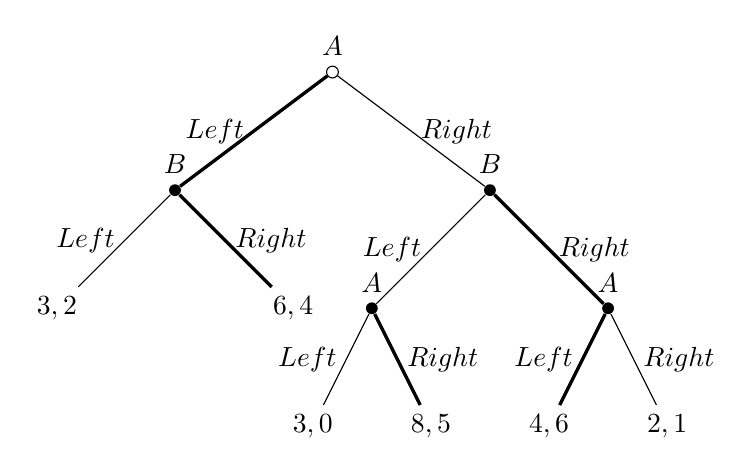
\begin{tikzpicture}[thin,
		level 1/.style={sibling distance=40mm},
		level 2/.style={sibling distance=30mm},
		level 3/.style={sibling distance=15mm},
		every circle node/.style={minimum size=1.5mm,inner sep=0mm}]
		
		\node[circle,draw,label=above:$A$] (root) {}
		child { node [circle,fill,label=above:$B$] (node-F) {}
			child { 
				node {$3,2$}
				edge from parent
				node[left] {$Left$}}
			child { 
				node (node-G) {$6,4$}
				edge from parent
				node[right] {$Right$}}
			edge from parent
			node[left] {$Left$}}
		child { node [circle,fill,label=above:$B$](node-E) {}
			child { 
				node[circle,fill,label=above:$A$](node-B) {}
				child {
					node {$3,0$}
					edge from parent
					node[left] {$Left$}}
				child {
					node (node-A) {$8,5$} 
					edge from parent
					node[right] {$Right$}}
				edge from parent
				node[left] {$Left$}}
			child { 
				node[circle,fill,label=above:$A$](node-C)  {}
				child {
					node (node-D) {$4,6$}
					edge from parent
					node[left] {$Left$}}
				child {
					node {$2,1$}
					edge from parent
					node[right] {$Right$}}
				edge from parent
				node[right] {$Right$}}
			edge from parent
			node[right] {$Right$}};
		\draw [very thick] (node-A) -- (node-B) 
		node[midway,above] {};
		\draw [very thick] (node-C) -- (node-D) 
		node[midway,above] {};
		\draw [very thick] (node-E) -- (node-C) 
		node[midway,above] {};
		\draw [very thick] (node-F) -- (node-G) 
		node[midway,above] {};
		\draw [very thick] (root) -- (node-F) 
		node[midway,above] {};
		\end{tikzpicture}
	\end{center}
	\caption{A game between players A and B}
\end{figure}

We can see in the figure below that the first player to act is Player A, at the root node. Her choices are to move \emph{Left} or \emph{Right}. Player B faces similar choices at the resulting nodes, and the players alternate turns until the game ends and they receive their payoffs, listed \emph{(A,B)}. Briefly glancing through the outcomes, it looks like A should aim for the node with payoff \emph{(8,5)}, because 8 is the highest payoff available to A. However, the official solution to the game is for A to first go \emph{Left}, and then for B to go \emph{Right}, resulting in a payoff of \emph{(6,4)}, where both get less than the intuitively appealing outcome! Why is this so?

Game theory makes strong assumptions about agent knowledge and rationality. The solution to this game is reached through an algorithm called \emph{backward induction}~\cite{VB_TowardPlay}. The players reason by starting at each end node and looking to the immediate parent node, and asking what the deciding player will do at that node, assuming she will choose the path with the highest payoff. So, at the bottom right of the figure, player A is to act, and she can go \emph{Left} for a payoff of 4, or \emph{Right} for a payoff of 2. So, she will go \emph{Left}, illustrated by the bold line. The end nodes not selected are subsequently eliminated. This process is repeated at each end node. Then it is recursively applied up the tree. So along the right branch, player B decides between \emph{Left} for a payoff of 5, or \emph{Right} for a payoff of 6, because B knows that A is rational, and he knows how she will act at each end node. A, at the root, then must choose between \emph{Left} for a payoff of 6, or \emph{Right} for a payoff of 4, because she knows that B is rational, and knows that B knows that she is rational. The explanation begins to illustrate the assumptions game theory makes about each player's knowledge. In fact, this only scratches the surface.

%The story is that Players A and B have been arrested for committing a crime together, and the prosecuting attorney offers them each the following deal: You and your partner in crime can either Defect from or Cooperate with each other. If you Defect and she Cooperates, I will let you go free, and come down hard on her with 10 years. If you both Defect, you will each get 6 years. If you both Cooperate with each other, I can only convict you of a lesser crime, which carries a sentence of 2 years. Some tellings assert that the defendants cannot communicate, but this does not matter under the classical model of rationality. No matter what the other does, each agent is better off by Defecting. Thus, the rational outcome of the game is for each agent to defect, each receiving 6 years. The counterintuitive aspect here is that if each agent have Cooperated, then they collectively would have been better off with 2 years each. But, this outcome cannot occur, because if one Cooperates, the other should Defect: 0 years is better than 2 years.

Game theory, and classical economics in general, makes the following assumptions about agent knowledge, formalized in epistemic logic~\cite{Aumann}. 

$\mathbf{Agency\  Model\  in\  Classical\  Game\  Theory}$.\\
(1) $\Kns{i}(\varphi \iimplies \psi) \iimplies (\Kns{i}\varphi \iimplies \Kns{i}\psi)$\\
(2) $\Kns{i}\varphi \iimplies \varphi$\\
(3) $\Kns{i}\varphi \iimplies \Kns{i}\Kns{i}\varphi$\\
(4) $\tlnot \Kns{i}\varphi \iimplies \Kns{i}\tlnot\Kns{i}\varphi$\\
(5) $\mathbf{C}_G ((1) \tland (2) \tland (3) \tland (4) \tland (5))$.

This forms an idealized model of the knowledge component of classical game theory's agents. $\Kns{i}$ is a modal operator for knowledge, and $\Kns{i}\varphi$ reads, ``agent \emph{i} knows that $\varphi$." $\mathbf{C}_G$ is a modal operator for common knowledge, the fixpoint for ``everyone in group G knows that everyone knows that..." The agents are logically omniscient due to (1), knowledge implies truth with (2), agents have \emph{positive introspection} with (3), and \emph{negative introspection} with (4). Assumptions (1), (3), (4), and (5) are somewhat dubious. The model also fails to formally represent other aspects of agency, like action and evaluation of outcomes. The model we propose makes weaker, more realistic assumptions about knowledge, includes a modal operator for belief, and formally represents action and the evaluation of actions as either safe or unsafe.

Recent work at the intersection of game theory and logic focuses on the information flow that occurs during games. Van Ditmarsch identifies a class of games called \emph{knowledge games}, in which players have diverging information~\cite{ditmarsch}. This slightly relaxes the assumption of classical game theory that players have common knowledge about each other's perfect information. Similarly, it invites logicians to study the information conveyed by the fact that an action is executed. For example, if the action is that agent $1$ asks agent $2$ the question, ``$p$?", the information conveyed is that $1$ does not know whether $p$, believes that $2$ knows whether $p$, and after the action occurs, this information becomes publicly known. The logic modeling games of this kind is of particular interest to us, as we are concerned with identifying the knowledge and belief state of human pilots based on their actions. 

The proceeding sections introduce the various logical systems that form a foundation for the work of this thesis, starting with modal logic in its traditional philosophical interpretation, and expanding to epistemic and doxastic logic. Then, we introduce dynamic logic, and its expansion into Dynamic Epistemic Logic and Public Announcement Logic.

\section{Modal Logic}\label{sec:logic_foundation}
Aristotle noted a distinction between contingent truth and necessary truth, and some Medieval philosophers continued this line of inquiry. Necessary truths could not have been otherwise. The definitions of natural numbers and the addition function guarantee that in all possible worlds, \emph{2 + 2 = 4}. On a plane, the truths of Euclidean geometry are necessarily true. ``There is life on Saturn's moon Enceladus" is a possible truth. ``Enceladus has water on it" is a contingent truth. What about ``Water is H20"? Modal logic was formalized in the early 1900's by C. I. Lewis and has recently had a resurgence in multidisciplinary interest~\cite{VB_MLOM}. At its core, modal logic allows us to reason about necessary and possible truths through the use of modal operators. What follows is a brief illustration of modal logic's concepts and formalisms.

When philosophers talk about necessity they usually mean \emph{metaphysical} necessity. In addition to formalizing this notion for systematic reasoning, modal logic is used for clarifying what exactly this means~\cite{Williamson}. Simple and intuitive examples are those from mathematics and notions of identity. Suppose $p$ is the arithmetic expression ``2 + 2 = 4". Obviously, $p$ is true in the actual world. We can make the stronger claim that $p$ is necessarily true, but what does this mean? As informal shorthands, initial attempts to define necessary truths might appeal, as I did above, to the claim that they could not possibly have been false. But then what do we mean by ``possible"? The formal semantics for dealing with these questions comes from Arthur Prior and Saul Kripke, and we introduce that machinery in the next section~\cite{Prior,Kripke}. For now, we say a statement is necessarily true if and only if it is true in all worlds we consider possible. The modal operator for necessity makes the formal statement: $\Box p$. Consider the following inference, where $\iimplies$ means ``implies": $\Box p \iimplies p$. This reads, ``Necessarily $p$ implies $p$," or equivalently, ``If $p$ is necessarily true, then $p$ is true." If $p$ is necessarily true, is $p$ true? Intuitively, the answer is `yes', and indeed a modal logic of metaphysical necessity includes this axiom for all formulas $\varphi$: $\Box \varphi \iimplies \varphi$. 

What other inferences can we make, based on our intuitive notion of necessity and possibility? What about ``if $p$ is true, then $p$ is possibly true"? To formalize this, we need the modal operator for possibility: $\Diamond$. So, the modal formula would be $p \iimplies \Diamond p$. This seems true as well, and indeed it is a theorem for metaphysical modal logic: $\varphi \iimplies \Diamond \varphi$. 
%In fact, those two axioms are equivalent. The definition of $\Diamond \equiv \tlnot \Box \tlnot$. This states that something is possible if and only if it is not necessarily false. It can also be said that something is necessary if and only if it is not possibly false: $\Box \equiv \tlnot \Diamond \tlnot$. We can now prove that the two axioms are equivalent.

%\begin{proof}
%	We first prove $\Box \varphi \iimplies \varphi$ implies $\varphi \iimplies \Diamond \varphi$, for any arbitrary $\varphi$ so long as it is the same on each side of the $\iimplies$. We begin by assuming $\Box \varphi \iimplies \varphi$. By the definition of $\Box$, we can substitute the equivalent formula $\tlnot \Diamond \tlnot \varphi \iimplies \varphi$. By contraposition, it holds that $\tlnot \varphi \iimplies \Diamond \tlnot \varphi$. But $\varphi$ is any arbitrary formula, including $\tlnot \varphi$. So we can substitute arbitrary formulas and get $\varphi \iimplies \Diamond \varphi$. What matters is that the $\varphi$ on the left and right of the $\iimplies$ are the same, not that they are the same in each axiom.
	
%	Next we prove that $\varphi \iimplies \Diamond \varphi$ implies $\Box \varphi \iimplies \varphi$, for arbitrary $\varphi$'s in each axiom. Assume $\varphi \iimplies \Diamond \varphi$. We can substitute in the equivalent formula using the definition of $\Diamond$ and get $\varphi \iimplies \tlnot \Box \tlnot \varphi$. By contraposition, it follows that $\Box \tlnot \varphi \iimplies \tlnot \varphi$. We substitute in $\varphi$ for $\tlnot \varphi$ as the arbitrary formula, and have $\Box \varphi \iimplies \varphi$.
%\end{proof}

It is obvious then that $\Box \varphi \iimplies \Diamond \varphi$ is a theorem. This states that if something is necessarily true then it is possibly true. What about the other direction: $\Diamond \varphi \iimplies \Box \varphi$? It turns out this is not a theorem under the typical notions of necessity and possibility. But this raises a question about how we would present a counterexample that disproves it. To do this, we need a semantics for the logic. The semantics we use are called \emph{possible world semantics}, and they are usually attributed to Saul Kripke~\cite{Kripke}. One would be hard-pressed to find a species of modal logic, whether in economics, computer science, or philosophy, that does not use possible world semantics in some form or another. Sometimes they are referred to as \emph{Kripke semantics}.

In possible world semantics, a graph structure is created with worlds as nodes and accessibility relations among worlds as the edges in the graph~\cite{modal}. Propositional formulas are true or false at each world. These graph structures are typically called Kripke structures. We can define the following Kripke structure, $\mathcal{M} = \{W, R, V\}$, where $W$ is a finite set of worlds, $\{w, v\}$, $R$ is a binary accessibility relation defined on those worlds $\{(w,v), (v,w)\}$, meaning $w$ has access to $v$ and $v$ has access to $w$, and $V$ is a \emph{valuation} function, which maps propositions to sets of worlds at which they are true. For example, if $p$ is true at $w$, then $w \in V(p)$. In our model we only care about the proposition $p$, which now stands for some contingent proposition, like ``all swans are white". Formally, we say $w \not\in V(p)$ if not all swans are white in world $w$, denoted by $\tlnot p$, while $w \in V(p)$ if they are, denoted by $p$. The following figure illustrates $\mathcal{M}$:

\begin{figure}[H]
	\begin{center}
	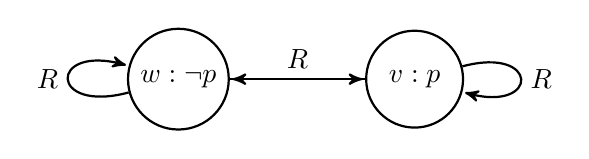
\begin{tikzpicture}[->,>=stealth',shorten >=1pt,auto,node distance=3cm,
	thick,base node/.style={circle,draw,minimum size=35pt}]
	
	\node[base node] (w) {$w: \tlnot p$};
	\node[base node] (v) [right of=w] {$v: p$};
	\path[]
	(w) edge node[above] {$R$} (v)
	    edge [loop left] node {$R$} (w)
	(v) edge node[below] {} (w)
%	\draw [->] (v) edge[in=5,out=355,loop] node[right] {$R$} (v)
	    edge [<-, loop right] node {$R$} (v);
	\end{tikzpicture}
	\end{center}
	\caption{$\mathcal{M}$: A simple counterexample using possible world semantics.}
\end{figure}

According to possible world semantics, $\Box \varphi$ is true at a world $w$, written $w \models \Box \varphi$, if and only if for all worlds $v$ such that $R(w,v)$ ($v$ is related to $w$ by the $R$ relation), $v \models \varphi$. This says a formula is necessarily true at a world if and only if it is true at all worlds accessible by that world according to the underlying $R$ relation. Similarly, $w \models \Diamond \varphi$ if and only if there is some world $v$ such that $R(w,v)$ and $v \models \varphi$. In $\mathcal{M}$, $w$ is $R$-accessible to itself, so there is a world accessible to $w$ where $p$ is false, and thus $w \models \tlnot \Box p$. However, since $v$ is $R$-accessible to $w$, and $v \models p$, it is true that $w \models \Diamond p$. Thus, we have $w \models \Diamond p$ and $w \models \tlnot \Box p$, a negation of $\Diamond p \iimplies \Box p$, so it cannot be the case that $\Diamond \varphi \iimplies \Box \varphi$ is a theorem, for arbitrary formula $\varphi$.

There are many systems of modal logic. The way any is distinguishedfrom  another is based entirely on the definition of $R$. For the popular \SFive, which we will examine later, $R$ is a Euclidean and eflexive binary relation on worlds. Thus, that is how ``possibility" is formally defined, and by extension, ``necessarily". That is also what determines the axioms and theorems comprising the logic. We formally define these notions in the next section, along with the syntax and semantics of propositional modal logic.

\subsection{Modal Logic Syntax and Semantics}~\label{sec:molo_syn_sem}
This section formally defines the syntax, what the logic looks like, and the semantics, what the truth conditions are for the logic.

Recall that Boolean logic is a simple logic for reasoning about basic propositions using the logical connectives `and', `or', `not', and `if...then'. It forms the foundation of most logics and has applications ranging from philosophy to circuit design. Propositions are represented as constants {\emph p,\ \emph q} and well-formed formulas of the language are constants and any proper combination of constants using the above logical connectives, represented symbolically as,
$$\varphi \stackrel{def}{=} p\  |\  \varphi \wedge \varphi\  |\  \varphi \vee \varphi\  |\ \neg \varphi \ |\   \varphi \iimplies \varphi. 
$$

As illustrated in the previous section, modal logic adds to propositional logic with modal operators for necessary and possible truths. The syntax for propositional logic is extended in the following way to make modal logic:


The semantics for Boolean logic are simply truth tables for each connective, which I will not reproduce here. However, the operators in modal logic are not truth functional, and require more complex semantics, which we earlier mentioned are called possible world semantics. They are as follows.

Let $\mathcal{M} = \{W, R, V\}$ be a model such that $W$ is a set of possible worlds, $R$ is a binary relation on those worlds, and $V$ is a valuation function mapping atomic propositions to the sets worlds satisfying them,  

\begin{align*}
w \models p\  &\mathbf{iff}\ w \in V(p) \\
w \models \neg \varphi\  &\mathbf{iff}\  w\not\models \varphi  \\
w \models \varphi \wedge \psi\ &\mathbf{iff}\ w\models \varphi\ \mathnormal{and}\ w\models \psi \\
w \models \Box \varphi\  &\mathbf{iff}\ \forall v,\ R(w,v)\  \mathnormal{implies}\ v \models \varphi. \\
w \models \Diamond \varphi\ &\mathbf{iff}\ \exists v,\ R(w,v)\ \mathnormal{and}\ v\models \varphi.
\end{align*}

The character of a modal logic is determined by the binary relation on worlds underlying the modal operators. We mentioned \SFive\ in the previous section as having a $R$ relation in which every world is accessible to itself by the binary relation. It is also one in which the $R$ relation is Euclidean. These conditions are called a \emph{frame} conditions, and the models that satisfy these conditions belong to said frame. All reflexive frames have the following frame conditions:
\begin{equation}
\forall x,\ R(x,x)
\end{equation}
Likewise, all reflexive frames have the following axiom:
\begin{equation}
	\Box \varphi \iimplies \varphi
\end{equation}
It is not just a stipulation that all reflexive frames must have that axiom: They have that axiom \emph{because} they have that frame condition. This is due to correspondence theory, which we explain later on.

Relaxing a frame condition changes the $R$ relation, and in doing so changes the logic. If we remove the reflexivity condition, the above axiom is no longer an axiom for the logic defined on $\mathcal{M}$. This means that we can specify the axioms we want by specifying the frame condition on the accessibility relation. Each frame condition corresponds to a modal logic axiom. In addition to reflexivity, the other common frame conditions are as follows, with their corresponding modal logic axiom:
\begin{itemize}
	\item Transitivity
	\begin{eqnarray}
	\forall x,y,z\ R(x,y) \tland R(y,z) \iimplies R(x,z)\\
	\Box \varphi \iimplies \Box \Box \varphi
	\end{eqnarray}
	\item Symmetry
	\begin{eqnarray}
	\forall x,y\ R(x,y) \iimplies R(y,x)\\
	\varphi \iimplies \Box \Diamond \varphi
	\end{eqnarray}
	\item Euclidean
	\begin{eqnarray}
	\forall x,y,z\ R(x,y) \tland R(x,z) \iimplies R(y,z)\\
	\Diamond \varphi \iimplies \Box \Diamond \varphi
	\end{eqnarray}
	\item Seriality
	\begin{eqnarray}
	\forall x \exists y, R(x,y) \\
	\Box \varphi \iimplies \Diamond \varphi
	\end{eqnarray}
\end{itemize}

These conditions are not exhaustive, but they represent some of the commonly combined conditions used to define axioms of different modal logics. By combining frame conditions, a modal operator is defined with the properties desired. For example, if we wish to define a modal operator for reasoning about the knowledge of ideally rational agents, as is done in Fagin \etal\cite{FHMV}, we impose the frame conditions of reflexivity and Euclidicity (Euclideanness), or one that is transitive and reflexive, as in Hintikka~\cite{Hintikka}. However, if we wish to develop a logic for belief, as the previously cited works also do, we must impose transitivity, Euclidicity, and seriality. The reasons for this are explored in the following sections.

\subsection{Epistemic Logic}~\label{epistemic_logic}
Epistemic logic began with philosophical concerns about knowledge ~\cite{FHMV,Hintikka,rescher}. Presently, it is likely to be studied in computer science as the logic for reasoning about ideally rational agents in well-structured environments. The agents are ideally rational in the sense that there is no bound on how much they can be said to know, nor on what propositions they are aware of at any one time. Thus, they have no problem conceiving of every possible sequence of moves a game may consist of, evaluating all possible outcomes, and deducing the optimal sequence of moves in order to maximize their own utilities. They are even stronger than contemporary computers in this way, which are bounded by time and space, and so are unable to actually compute the ideal strategy for an otherwise solvable game like Go. An ideally rational agent can solve Go and compute the game tree all the way to its end. These are the agents of game theory, which always select the optimal move when they have perfect information about the game and the other players.

The axioms that specify this level of knowledge are those introduced in Section~\ref{gametheory}, and recounted here without reference to common knowledge, which complicates things too much for our purposes:

$\mathbf{Agency\  Model\  in\  Classical\  Game\  Theory}$.\\
(1) $\Kns{i}(\varphi \iimplies \psi) \iimplies (\Kns{i}\varphi \iimplies \Kns{i}\psi)$\\
(2) $\Kns{i}\varphi \iimplies \varphi$\\
(3) $\Kns{i}\varphi \iimplies \Kns{i}\Kns{i}\varphi$\\
(4) $\tlnot \Kns{i}\varphi \iimplies \Kns{i}\tlnot\Kns{i}\varphi$.

These axioms make the knowledge operator an $\mathit{S5}$ modal operator. Strictly speaking, including (3) is unnecessary because it follows as a theorem from (2) and (4), but we include it so that the reader is not surprised when we refer to it.

The first axiom holds for all \emph{normal} modal logics, and under the epistemic interpretation, it states that if an agent knows that $\varphi$ implies $\psi$, and she knows $\varphi$, then she knows $\psi$. This is intuitive enough on the first pass, but can lead to a problem of global skepticism. If $i$ knows that she is an embodied agent in the external world only if she knows that she is not a brain in a vat perceiving a simulated reality, then she knows she is an embodied agent only if she knows she is not a brain in a vat. It seems clear that she cannot know that she is not a brain in a vat, because her sensory experience is compatible with either the embodied scenario of the brain in a vat scenario. Therefore, she does not know she is an embodied agent in the external world. Thus, many philosophers question whether knowledge for human-like agents is closed under logical implication like this.

The second axiom states that a known proposition must be true, and finds ample support from philosophers devoted to studying the nature of knowledge. It can be considered the property of knowledge that most distinguishes it from belief, because beliefs can be false.

The third axiom, \emph{positive introspection}, states that an agent knows something only if she knows \emph{that} she knows it. This imposes a high standard on knowledge, under the assumption that an agent can identify the conditions that guarantee the truth of a known proposition, and in being able to do so, are justified to a sufficient degree. However, this property is largely rejected by philosophers, as this requirement is thought to be largely unattainable. 

Finally, \emph{negative introspection} states that an agent does not know something only if she knows that she does not know it. This has an undesirable effect of creating knowledge out of ignorance, for if $i$ does not know that she does not know $\varphi$, this is sufficient for inferring that she knows $\varphi$, according to negative introspection. This is fine for ideally rational agents, and indeed it is a noble aspirational goal to know what one is ignorant about, but for human-like agents it is entirely unrealistic as an axiom.

These axioms are firmly rooted in the literature of formal epistemology and epistemic logic, and relaxing them in order to model more realistic agents requires a word or two. This section introduces and defends our relaxation of the classical axiomatization.

\subsection{Why S5 Is Appealing} 
Before presenting our relaxed axiom schema for knowledge, we acknowledge the appealing properties of the S5 knowledge operator. Logicians who adopt the S5 knowledge operator have good reasons for doing so, both technical and intuitive. The technical appeal lies in the fact that the S5 operator is well-behaved from a logical point of view. Epistemic logics with S5 operators are decidable because S5 operators have semantics that satisfy the finite model property, meaning that every invalid proposition has a finite counter-model. The S5 knowledge operator allows a formula prefixed by any arbitrary combination of $\Kns{i}$, and its dual $\Poss{i}\equiv\tlnot\Kns{i}\tlnot$, symbols to be reduced to a formula prefixed by at most two. This keeps the models small.

On the intuitive side, the relations that define the semantics of an S5 knowledge operator are equivalence relations. They are defined as reflexive and Euclidean, which implies that they are also transitive and symmetric. Equivalence relations capture a notion of indistinguishability because each world in the equivalence class is indistinguishable from each other. All the modal formulas true at one of the worlds in an equivalence relation are true at each of the other worlds in the relation, so from a modal perspective, they are indistinguishable. When the modality is knowledge, this means that relative to the agent's knowledge, the worlds are indistinguishable. 

These properties of \SFive\ epistemic logic are strong points in its favor. We suppose that any formal system seeking to model human-like knowledge must capture the intuitive idea that an agent does not know \emph{whether} a proposition $\varphi$ is true or false just in case she cannot distinguish the world she is in from the possible worlds in which either might be the case. Distinguishability seems to imply that there is some evidence possessed by the agent that allows her to rule out possibilities, and therefore gain knowledge.

The technical benefit of the finite model property makes \SFive\ a friendly logic to work with, but it is not a reason to believe that the theory of knowledge described by \SFive\ is true of human agents. Therefore, we do not see the need to impose this condition as a requirement for realistic epistemic logics. However, it would be desireable to achieve the finite model property while maintaining realism.

Next we turn to a brief summary of doxastic logic, which shall play a role in \DASL's static foundation. 

\subsection{Doxastic Logic}
This section presents doxastic logic, the logic for reasoning about belief. Hintikka's formalization in \cite{Hintikka} of the belief operator is standard, and we adopt it here. The operator $\Bels{i}$ for `agent $i$ believes $\ell$' is defined by a binary relation on worlds that is serial and Euclidean. It is a normal modal operator, and the property of transitivity follows from seriality and Euclidicity. So, the model of an agent's belief is defined by the following axioms,

$\mathbf{Hintikka\ Belief\ Model}$.\\
(1) $\Bels{i}(\varphi \iimplies \psi) \iimplies (\Bels{i}\varphi \iimplies \Bels{i}\psi)$\\
(2) $\Bels{i}\varphi \iimplies \BPoss{i}\varphi$\\
(3) $\Bels{i}\varphi \iimplies \Bels{i}\Bels{i}\varphi$\\
(4) $\tlnot \Bels{i}\varphi \iimplies \Bels{i}\tlnot\Bels{i}\varphi$.

Clearly the primary difference between this model of belief and the model of knowledge from classical game theory is axiom (2). Rather than guaranteeing truth, beliefs guarantee consistency. One could correctly argue that this is too strong of an assumption for humans, but we leave relaxations of the belief model to future work, and are content to relax the idealizations about knowledge in this dissertation. Similarly, reasonable cases could be made against axioms (3) and (4).

The logic associated with these axioms is called $\mathcal{KD}\mathit{45}$. On the doxastic interpretation, it represents a slight idealization of how humans actually adopt beliefs. Clearly, humans can have contradictory beliefs, and they may believe something without believing that they believe it. Cases of cognitive dissonance like that are idealized away, not only because modeling such a psychology is complicated, but also because we seek a logic that maintains some level of normativity. If someone believes two contradictory propositions, she should be able to give one up if this contradiction is pointed out to her, and furthermore she is rational to do so. This reflects Hintikka's goal of developing logics of knowledge and belief that allow us to consistently identify when attributions of knowledge and belief are in some sense criticizable. Maintaining a notion of normativity in a logic is important to us, and underlies some the idealizations we accept in \DASL's static base logic.

Knowledge involves a condition that is external to the agent's direct perception: the truth or falsity of the proposition. Belief, on the other hand, is entirely internal to the agent's perception. She can introspect on her evidence and deliberate on a proposition, and this is sufficient to see that she believes or disbelieves it, and this attitude is immediately available to her. For this reason, the positive and negative introspection axioms are more appropriate for belief than they are for knowledge. 

\subsection{Knowledge and Belief Combined}
In addition to developing a stand-alone axiomatization of the belief operator, Hintikka combined the knowledge and belief operators into a single multi-modal system. Other philosophers and logicians have constructed similar systems. Hintikka considers the following combined axioms, which he calls conditions, as options:

$\mathbf{Hintikka\ Combinations\ Considered}$.\\
(1) $\Kns{i}\varphi \iimplies \Bels{i}\Kns{i}\varphi$\\
(2) $\Kns{i}\varphi \iimplies \Bels{i}\varphi$\\
(3) $\Bels{i}\varphi \iimplies \Kns{i}\Bels{i}\varphi$\\
(4) $\Bels{i}\varphi \iimplies \Kns{i}\varphi$.

He subsequently rejects (4) immediately, and through deliberation (3), while he accepts (1) and (2). Thus, Hintikka's combined logic of knowledge and belief is,

\begin{table}[H]
	\begin{center}
		\begin{tabular}{| l r |}
			\hline
			$\Kns{i}(\varphi \iimplies \psi) \iimplies (\Kns{i}\varphi \iimplies \Kns{i}\psi)$ & Distribution of $\Kns{i}$ \\
			$\Kns{i}\varphi \iimplies \varphi$ & Truth Axiom \\
			$\Kns{i}\varphi \iimplies \Kns{i}\Kns{i}\varphi$ & Positive Knowledge Introspection\\
			$\Bels{i}(\varphi \iimplies \psi) \iimplies (\Bels{i}\varphi \iimplies \Bels{i}\psi)$ & Distribution of $\Bels{i}$\\
			$\Bels{i}\varphi \iimplies \BPoss{i}\varphi$ & Belief Consistency Axiom\\
			%			$\Bels{i}\varphi \iimplies \Bels{i}\Bels{i}\varphi$ & Positive Belief Introspection \\
			$\tlnot\Bels{i}\varphi \iimplies \Bels{i}\tlnot\Bels{i}\varphi$ & Negative Belief Introspection\\
			$\Kns{i}\varphi \iimplies \Bels{i}\varphi$ & Knowledge implies Belief \\
			$\Kns{i}\varphi \iimplies \Bels{i}\Kns{i}\varphi$ & Undeniable Knowledge\\
			%			$\Bels{i}\varphi \iimplies \Kns{i}\Bels{i}\varphi$ & Beliefs are Known\\
			From $\vdash \varphi$ and $\vdash \varphi \iimplies \psi$, infer $\vdash\psi$ & Modus Ponens\\
			From $\vdash \varphi$, infer $\vdash \Kns{i}\varphi$ & Necessitation of $\Kns{i}$\\
			\hline
		\end{tabular}
		\caption{Hintikka's Combined Logic of Knowledge and Belief}
	\end{center}
\end{table}

We omit his defense of positive knowledge introspection, but point out that his defense of undeniable knowledge depends on his interpretation of the operators. Hintikka is concerned in his project with identifying statements about knowledge and belief that utterers cannot defensibly deny. Furthermore, his interpretation of knowledge and belief are not those propositions actively held in one's head, but those to which one could be led through a series of applications of \emph{Modus Ponens} from what one already knows or believes. We can think of knowledge, for Hintikka, as those propositions implied by what one already knows, and beliefs as those propositions that one is logically committed to by one's beliefs. This avoids the problem of logical omnicience for both modal operators. And it sets up an argument like the following, 
\begin{enumerate}
	\item $\varphi$ follows logically from what $i$ knows
	\item If (1) is pointed out to $i$, it is indefensible for $i$ to deny that she believes that she knows $\varphi$.
	\item Therefore, $\Kns{i}\varphi \iimplies \Bels{i}\Kns{i}\varphi$
\end{enumerate}

For Hintikka, this suffices to accept the formula as valid, as well as Knowledge implies Belief, for which a similar argument can be presented.

Conversely, Hintikka rejects (3) because he does not find it plausible that \\$\Bels{i}\varphi \iimplies \Kns{i}\Poss{i}\varphi$, which (3) and the Truth Axiom jointly imply. He furthermore rejects arguments from introspection, which might ground a defense in considered formula (3), as fallacious. 

Another potential combined logic of knowledge and belief is due to Kraus and Lehmann in \cite{KrausLehmann}.

\begin{table}[H]
	\begin{center}
		\begin{tabular}{| l r |}
			\hline
			$\Kns{i}(\varphi \iimplies \psi) \iimplies (\Kns{i}\varphi \iimplies \Kns{i}\psi)$ & Distribution of $\Kns{i}$ \\
			$\Kns{i}\varphi \iimplies \varphi$ & Truth Axiom \\
			$\Kns{i}\varphi \iimplies \Kns{i}\Kns{i}\varphi$ & Positive Knowledge Introspection\\
			$\tlnot\Kns{i}\varphi \iimplies \Kns{i}\tlnot\Kns{i}\varphi$ & Negative Knowledge Introspection\\
			$\Bels{i}(\varphi \iimplies \psi) \iimplies (\Bels{i}\varphi \iimplies \Bels{i}\psi)$ & Distribution of $\Bels{i}$\\
			$\Bels{i}\varphi \iimplies \BPoss{i}\varphi$ & Belief Consistency Axiom\\
			%			$\Bels{i}\varphi \iimplies \Bels{i}\Bels{i}\varphi$ & Positive Belief Introspection \\
%			$\tlnot\Bels{i}\varphi \iimplies \Bels{i}\tlnot\Bels{i}\varphi$ & Negative Belief Introspection\\
			$\Kns{i}\varphi \iimplies \Bels{i}\varphi$ & Knowledge implies Belief \\
			$\Bels{i}\varphi \iimplies \Kns{i}\Bels{i}\varphi$ & Known Belief\\
			%			$\Bels{i}\varphi \iimplies \Kns{i}\Bels{i}\varphi$ & Beliefs are Known\\
			From $\vdash \varphi$ and $\vdash \varphi \iimplies \psi$, infer $\vdash\psi$ & Modus Ponens\\
			From $\vdash \varphi$, infer $\vdash \Kns{i}\varphi$ & Necessitation of $\Kns{i}$\\
			\hline
		\end{tabular}
		\caption{Kraus-Lehmann Combined Logic of Knowledge and Belief}
	\end{center}
\end{table}

Knowledge is \SFive\ and belief is based on a serial relation. However, from this system the remaining $\mathit{KD45}$ formulas are derivable. Additionally, they have the interesting theorem $\Kns{i}\varphi \equiv \Bels{i}\Kns{i}\varphi$. 

Kraus and Lehmann identify the formula $\Bels{i}\varphi \iimplies \Bels{i}\Kns{i}\varphi$ as interesting but exclude it, as it would cause a collapse of knowledge and belief into equivalence: $\Kns{i}\varphi \equiv \Bels{i}\varphi$. Obviously, a logic combining knowledge and belief should treat them as distinct operators, and we treat the avoidance of this collapse as a desirable feature of our own static base for \DASL. We also include the interesting formula above as an axiom, which imposes a condition on agents' beliefs that we consider a desireable idealization. To say $i$ believes $\varphi$ only if she believes that she knows $\varphi$ is to say she believes only those things that she has very good evidence for. This helps prevent agents from believing things without evidence, which we want to exclude from our model. The challenge with this axiom, as Kraus and Lehmann note, is to avoid the knowledge-belief collapse. We give this further treatment in a later chapter.

This concludes our discussion of static epistemic and doxastic logics, including their combination. We pick this thread back up later when we present the static base of \DASL. The next section presents the relevant background of dynamic extensions to epistemic logic.

%This is formalized in a couple different ways in the literature, sometimes as we did before mapping a proposition-world pair to a Boolean, sometimes defining propositions as sets of worlds, where $V(w)\in p$ if and only if $p$ is true at world $w$. The former convention will be followed here.



%\subsection{Avionics and Formal Methods}
%\section{Logical Framework}~\label{logic_foundation}
%This section introduces the logic used as a tool to formally model and reason about pilots in emergency situations. For most readers the logic to be used will be sufficiently complex and unfamiliar that a gradual approach is warranted, beginning with the basics of familiar Boolean logic, and advancing to the final logic specially developed for reasoning about pilot error.
%\subsection{Logical Foundations} 
%Recall that Boolean logic is a simple logic for reasoning about basic propositions using the logical connectives `and', `or', `not', and `if...then'. It forms the foundation of most logics and has applications ranging from philosophy to circuit design. Propositions are represented as constants {\emph p,\ \emph q} and well-formed formulas of the language are constants and any proper combination of constants using the above logical connectives, represented symbolically as,
%$$\varphi \stackrel{def}{=} p\  |\  \varphi \wedge \varphi\  |\  \varphi \vee \varphi\  |\ \neg \varphi \ |\   \varphi \rightarrow \varphi. 
%$$

%Boolean logic is limited in what it can express, however. Some situations require higher fidelity, for example when reasoning about knowledge. Consider the proposition, ``If Alice knows $p$, then $p$ is true." Philosophers of knowledge agree with this proposition, considering it a valid claim about knowledge, based on the principle that all known propositions are true. However, this validity cannot be faithfully represented in propositional logic as a general validity. Each sentence in the claim is assigned its own constant, resulting in a formalization like, ``$\mathit{a} \rightarrow \mathit{p}$," with {\emph a} representing ``Alice knows $p$," and $p$ representing ``$p$ is true." But $\mathit{a} \rightarrow \mathit{p}$ is not a validity of Boolean logic. 

%To represent reasoning about knowledge, and other similar domains requiring higher fidelity, epistemic operators are added to the basic Boolean logic, resulting in the following logic:

%$$\varphi \stackrel{def}{=} p\  |\ \mathbf{K_{i}}\varphi\ |\ \neg \varphi\ |\ \varphi \wedge \varphi, 
%$$
%where $\mathbf{K_{i}}\varphi$ states that agent ${\boldmath i}$ \emph{knows} that \emph{$\varphi$}, allowing us to formally represent the above validity:
%$$\mathbf{K_{Alice}}p \rightarrow p.$$

%Semantics for epistemic logic are given by Kripke structures, which serve as models by which epistemic formulas are evaluated. At its core, a Kripke structure is a graph with nodes and edges, accompanied by a function determining which atomic propositions are true at which worlds. The nodes are normally thought of as possible worlds, or as possible states of the system being modeled. The edges are normally thought of as possibility relations among worlds or states. If, at a node representing a world {\emph w}, agent {\emph A} considers it possible that she is in world {\emph v}, the Kripke semantics modeling this situation would have world {\emph w}'s node connected to world {\emph v}'s node by an edge representing {\emph A}'s epistemic possibility relation.

%Formally, we say a Kripke structure is a \emph{tuple} $\langle W,\ V,\ Agents,\ \{R_{i}|i\in Agents\}\rangle,$ where \emph{W} is a set of worlds, \emph{V} is a function from propositional constants to sets of worlds satisfying the proposition, \emph{Agents} is a set of agents, and each $R_{i}$ is agent \emph{i}'s epistemic possibility relation.

%The semantics are as follows, for worlds $w,\ v\ \in W$:
%\begin{align*}
%w \models p\  &\mathbf{iff}\ w \in V(p) \\
%w \models \neg \varphi\  &\mathbf{iff}\  w\not\models \varphi  \\
%w \models \varphi \wedge \psi\ &\mathbf{iff}\ w\models \varphi\ \mathnormal{and}\ w\models \psi \\
%w \models \mathbf{K_{i}}\varphi\  &\mathbf{iff}\ \forall v,\ wR_{i}v\  \mathnormal{implies}\ v \models \varphi.
%\end{align*}

%Early applications of epistemic logic in information security modeled system components as agents whose knowledge represented the information flowing to them. Recently, a modified version of epistemic logic known as dynamic epistemic logic has been used in information security to formally reason about security properties involving human components of systems. The research described in this proposal advances along similar lines, treating pilots as human components of safety critical aviation systems and using dynamic epistemic logic to reason about them. The next section describes the basic dynamic epistemic logic.

\section{Dynamic Epistemic Logic}~\label{sec:delsection}
This section presents the so-called \emph{dynamic turn} in modal logic, which incorporates elements of propositional dynamic logic into epistemic logic in order to model knowledge and action. See van Benthem \cite{VB_LDII,VB_MLOM,VB_TowardPlay}, and van Ditmarsch, van der Hoek, and Kooi \cite{DEL} for detailed examinations. The related Public Announcement Logic (PAL) uses similar techniques to model information flow among agents. See Baltag, Moss, and Solecki in \cite{BMS} for more on this.

Dynamic Epistemic Logic (DEL) formalizes situations in which agents' epistemic states change over time, due to announcements or other informational events\cite{DEL}. For example, if Alice truthfully and trustworthily communicates to Bob that $\varphi$, then after this informational even it is true that Bob knows $\varphi$. This situation cannot be modeled by the epistemic logic introduced in the previous section. To model it, we introduce the following formal machinery.

To capture informational events, we introduce the idea of relativizing a Kripke structure. In the previous example, if we model the Alice and Bob situation prior to Alice's communication, we can have a world $w$ from which Bob considers $\varphi$- as well as $\neg\varphi$-worlds possible. However, after the informational event, Bob knows $\varphi$, so the model is \emph{relativized} to a submodel in which only $\varphi$-worlds are accessible by Bob's epistemic possibility relation. Thus, after the informational event, the model transitions to a submodel with fewer edge relations.

The logic for reasoning about information flow in knowledge games is called Dynamic Epistemic Logic (DEL). As its name suggests, it combines elements of epistemic logic and dynamic logic. Epistemic logic is the static logic for reasoning about knowledge, and dynamic logic is used to reason about actions. In dynamic logic semantics, nodes are states of the system or the world, and relations on nodes are transitions via programs or actions from node to node. If we think of each node in dynamic logic as being a model of epistemic logic, then actions become relations on models, representing transitions from one multi-agent epistemic model to another. For example, if we have a static epistemic model $M1$ representing the knowledge states of agents Alice and Bob at a moment, then the action $``\varphi"$ is a relation between $M1$ and $M2$, a new static epistemic model of Alice's and Bob's knowledge after the question is asked. All of this is captured by DEL.

\begin {center}
\begin {tikzpicture}[-latex ,auto ,node distance =3 cm and 4cm ,on grid ,
semithick ,
state/.style ={ circle ,top color =white , bottom color = white ,
	draw, text=black , minimum width =1 cm}]

\node[state] (A)  {$M1$};
\node[state] (B) [right =of A] {$M2$};

\path (A) edge  node[above] {$``\varphi"$} (B);
%\path (C) edge [bend left =25] node[below =0.15 cm] {$1/2$} (A);
%\path (A) edge [bend right = -15] node[below =0.15 cm] {$1/2$} (C);
%\path (A) edge [bend left =25] node[above] {$1/4$} (B);
%\path (B) edge [bend left =15] node[below =0.15 cm] {$1/2$} (A);
%\path (C) edge [bend left =15] node[below =0.15 cm] {$1/2$} (B);
%\path (B) edge [bend right = -25] node[below =0.15 cm] {$1/2$} (C);
\end{tikzpicture}
\end{center}


The above figure illustrates the relationship between static epistemic models and dynamic logic models. As a purely dynamic model, the figure shows the action $``p?"$ transitioning between nodes $M1$ and $M2$. If we zoom in on the nodes, we see their structure as epistemic models, with their own nodes and edges, representing possible worlds and epistemic relations.
\begin{figure}[H]
\begin{center}
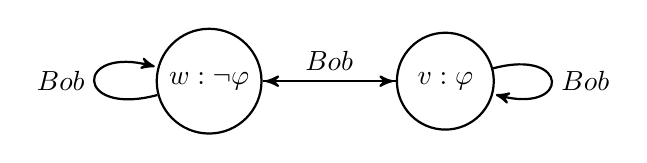
\begin{tikzpicture}[->,>=stealth',shorten >=1pt,auto,node distance=3cm,
thick,base node/.style={circle,draw,minimum size=35pt}]

\node[base node] (w) {$w: \tlnot \varphi$};
\node[base node] (v) [right of=w] {$v: \varphi$};
\path[]
(w) edge node[above] {$Bob$} (v)
edge [loop left] node {$Bob$} (w)
(v) edge node[below] {} (w)
%	\draw [->] (v) edge[in=5,out=355,loop] node[right] {$R$} (v)
edge [<-, loop right] node {$Bob$} (v);
\end{tikzpicture}
\end{center}
\caption{$M1$: The model before Alice announces $``\varphi"$.}
\end{figure}

\begin{figure}[H]
	\begin{center}
		\begin{tikzpicture}[->,>=stealth',shorten >=1pt,auto,node distance=3cm,
		thick,base node/.style={circle,draw,minimum size=35pt}]
		
		\node[base node] (v) [right of=w] {$v: \varphi$};

		\end{tikzpicture}
	\end{center}
	\caption{$M2$: The model after Alice announces $``\varphi"$.}
\end{figure}

We are concerned with an additional element: the \emph{safety} status of an action, and an agent's knowledge and belief about that. To capture this, we extend DEL and call the new logic Dynamic Agent Safety Logic (\DASL), which we introduce in the next chapter. The next section lays out the state of formal methods involving human-machine systems.

\section{Formal Methods Tools}~\label{sec:fm}

This section describes the Coq Proof Assistant \cite{coq_ref} and that this dissertation makes use of. We use Coq to mechanically check our metatheory proofs of soundness and completeness, and our object theory proofs about safety-critical information flow. Insofar as this thesis constitutes a work of logic or formal philosophy, we hope it can serve as an example for how to use formal tools to increase the rigor of research in these areas.

The Coq Proof Assistant is a combination of a dependently-typed functional programming language and a language of tactics for partially automating proof verification. Coq supports compilation to Haskell and OCaml, which is convenient because one can write a program and verify its correctness in Coq, then compile the code to a nicer implementation language. This dissertation does not take advantage of that feature. Instead, we embed \DASL\ in Coq and use it as a proof checker that allows us to write recursive functions and proof-automating tactics. This represents a use case of formal verification tools that one does not often see in the philosophy, mathematics, or logic departments of academia. Coq is a tool for us to use to increase the rigor of our research. Many who have ventured into the realm of mechanical theorem proving have been surprised initially by how complicated proofs `by routine induction' can become once all of the details must be spelled out, and indeed one can discover embarrassing mistakes when forced to spell out each detail.

%We use Z3 in the same way. As a tool, it is a collection of symbolic reasoning engines, including simplex, rewriting, DPLL, superposition, Euclidean solver, and others.\footnote{Presentation by Dr. Leonardo DeMoura, ``From Z3 to Lean: Efficient Verification." } We use it to validate that one can encode an instrument reading configuration and a safety precondition for an input action, and automatically detect whether the safety precondition is satisfied by the instrument readings. This validates an important requirement for implementing tools based on \DASL. Thus, rather than using Z3 to verify correctness properties of a prototype, we use it as an inference engine that demonstrates real time inference of safety-critical information from unsafe input actions.

The field of formal methods grew out of attempts to verify the correctness of hardware and software. It was normally confined to systems deemed mission- or safety-critical, due to its high cost. Arguments for the use of formal methods normally involve an anecdote in which a system fails due to some sort of error missed by traditional testing methods but that would have been caught and prevented were formal methods used.

Formal methods increase confidence that hardware and software components function correctly~\cite{RushbyFMbook}. They involve the application of mathematical techniques to the design and analysis of systems, usually the safety-critical components~\cite{johnson_butler_fm}. A standard approach is to develop an abstract specification of the software or hardware system, design the system to meet those specifications, and then use formal logic to prove that the designed system meets the desired safety specifications.

Recent concerns with AI safety from Yudkowsky \cite{yudkowski} and Bostrom \cite{bostrom} in particular highlight the need for formal methods that address correctness of AI software. Among the many challenges associated with this endeavor, one is the ability to formally model the AI agents themselves. By hypothesis, checking the correctness of these systems after they have been built is insufficient, so a formal language for specifying correctness properties is also needed. We do not pretend to provide a solution to these problems in this thesis, but we take modest steps in that direction.

By carefully choosing our axiom schemas, we construct a model of a human-like reasoner, and we show that we can specify formal properties about these reasoners. We do so with mechanization in Coq, which future work might be able to leverage through compilation to Haskell, OCaml, or some other functional language that preserves correctness proved in Coq.

Additionally, the use of formal tools like Coq to model human-like agency offers opportunities for philosophers to formalize and explore the implications of their theories. Sometimes merely attempting to formalize a theory and failing will be a valuable contribution to say, epistemology. Rigorously formalizing arguments and checking their validity could be another use of this technology, and it has been used for example by Rushby in \cite{rushby_ontological}, where he mechanizes Anselm's onotological argument for the existence of God, and in doing so reveals some specious aspects. We hope our chapter on the philosophical considerations underlying epistemic logics contribute to the further adoption of formal tools for philosophical analysis.

This concludes our discussion on formal methods as they relate to our thesis. In the next chapter, we present \DASL\ and argue for its adoption over other epistemic logics for reasoning about human-like agents.

%According to the Federal Aviation Administration (FAA), one of the top 12 causes of mistakes in the aviation workplace is a lack of awareness~\cite{faa}. According to Boeing and the FAA, approximately 80 per cent of aviation accidents (including maintenance accidents) are due to human error~\cite{boeing,faaHF}. To increase safety in human factors, the industry relies on education, psychology, anthropometrics, safety engineering, and to a limited extent, computer science. The primary focus of computer science research regarding human factors is the design and testing of software systems that are easy and intuitive for humans to interact with. 

%Formal methods are traditionally deployed in one of two ways. The more painful but perhaps more commonly used approach is to perform \emph{semantic archeology}, wherein an artifact that has already been constructed is formalized into a mathematically rigorous language and then reasoned about. The way urged by most contemporary researchers involves continuously specifying and verifying correctness throughout the development process, prior to system deployment. To facilitate this preferred approach, most formal methods researchers devote themselves to developing tools that are easier to use in order to lower the barrier to entry and increase adoption.
%
%The intended use of these tools, however, has remained the same: to verify the correctness of hardware and software systems, or to provide assistance to mathematicians attempting to prove theorems. At bottom, the tools allow computers to provide assistance to humans who are attempting to prove or disprove mathematical theorems.
%
%Thus we have a situation in which formal methods researchers advocate for the use of formal methods due to the inherent uncertainties involved with empirical testing of systems. However, they are satisfied to leave validation of the human component, the most risky component, to empirical testing.

%Some researchers have sought to develop formal methods for mitigating human-induced sources of failure~\cite{ButlerModeConfusion,Rushby_Mode_Confusion}. Thus far this work has focused on the development of formal methods tools for analyzing human machine interaction during the design and specification phase, rather than at runtime. The goals have been to develop software, and techniques for verifying the correctness of that software, to avoid mode confusion, a type of pilot error wherein the pilot believes the autopilot is in one mode, when in reality it is in another. In these situations, the autopilot is not offering protections concerning flight control inputs like thrust and pitch, so the pilot risks providing dangerous inputs.

%Butler, Miller, Potts, and Carreno~\cite{ButlerModeConfusion} trace mode confusion to three sources:
%\begin{enumerate}
%	\item poor display of automation state
%	\item unnecessarily complex automation
%	\item flight crew has an incorrect mental model of the state of the aircraft
%\end{enumerate}

%\noindent They say human factors research focuses on mitigating item (1) above, and they develop formal models in the PVS automated theorem prover to address items (2) and (3). However, the formal models they develop are of the automation system, not of the human components.

%In developing a realistic model of a human component that is capable of making mistakes, we lay a foundation for formal researchers to build tools that can identify and correct those mistakes at runtime.

%Similarly, Rushby~\cite{Rushby_Mode_Confusion} describes a class of errors he calls automation surprises, which are distinct but related to mode confusion. These occur when a pilot becomes surprised by the automated behavior of the system. He proposes a formal method addressing automation surprises that constructs a model of the system behavior, constructs a formal specification of a possible pilot's mental model of the system, and compares them for disagreement. His solution focuses on identifying potential automation surprises in the system, and both models are of the system behavior itself: one directly of the model, and one indirectly of the model, mediated through a hypothetical pilot's mind.

%In each of the above cases, the formal efforts focus on modeling the system itself, rather than on the human component, and they address the problem at design time. This work complements theirs by constructing a formal model of the pilot herself, and addressing the problem at runtime. Similarly, this work aims to address a variety of problems due to a pilot's loss of situational awareness, including mode confusion. The next chapter introduces Dynamic Agent Safety Logic.
\chapter{Dynamic Agent Safety Logic}
	\label{CH_03}


The logic for reasoning about information flow in knowledge games is called Dynamic Epistemic Logic (DEL). As its name suggests, it combines elements of epistemic logic and dynamic logic. Epistemic logic is the static logic for reasoning about knowledge, and dynamic logic is used to reason about actions. In dynamic logic semantics, nodes are states of the system (or of the world), and relations on nodes are transitions via programs or actions from node to node. If we think of each node in dynamic logic as being a model of epistemic logic, then actions become relations on models, representing transitions from one multi-agent epistemic model to another. For example, if we have a static epistemic model $M1$ representing the knowledge states of agents $1$ and $2$ at a moment, then the action $``p?"$ is a relation between $M1$ and $M2$, a new static epistemic model of $1$'s and $2$'s knowledge after the question is asked. All of this is captured by DEL.

\begin {center}
\begin {tikzpicture}[-latex ,auto ,node distance =3 cm and 4cm ,on grid ,
semithick ,
state/.style ={ circle ,top color =white , bottom color = white ,
	draw, text=black , minimum width =1 cm}]

\node[state] (A)  {$M1$};
\node[state] (B) [right =of A] {$M2$};

\path (A) edge  node[above] {$``p?"$} (B);
%\path (C) edge [bend left =25] node[below =0.15 cm] {$1/2$} (A);
%\path (A) edge [bend right = -15] node[below =0.15 cm] {$1/2$} (C);
%\path (A) edge [bend left =25] node[above] {$1/4$} (B);
%\path (B) edge [bend left =15] node[below =0.15 cm] {$1/2$} (A);
%\path (C) edge [bend left =15] node[below =0.15 cm] {$1/2$} (B);
%\path (B) edge [bend right = -25] node[below =0.15 cm] {$1/2$} (C);
\end{tikzpicture}
\end{center}

The above figure illustrates the relationship between static epistemic models and dynamic logic models. As a purely dynamic model, the figure shows the action $``p?"$ transitioning between nodes $M1$ and $M2$. If we were to zoom in on the nodes, we would see their structure as epistemic models, with their own nodes and edges, representing possible worlds and epistemic relations.

We are concerned with an additional element: the \emph{safety} status of an action, and an agent's knowledge and belief about that. To capture this, we extend DEL and call the new logic Dynamic Agent Safety Logic (DASL). The remainder of this section presents DASL's syntax, semantics, and proves its soundness. 
\section{Syntax and Semantics}
\subsection{Syntax}
The Dynamic Agent Safety Logic (DASL) used in this paper has the following syntax.
%, combining elements of Dynamic Epistemic Logic (DEL) and Agent Safety Logic (ASL).
\begin{tcolorbox}
	$$ \varphi \ ::=\   \lpp  \bnf \tlnot \varphi \bnf \varphi \tland \varphi  \bnf \Kns{i} \varphi \bnf \Bels{i}\varphi \bnf \Pal{i, (A,\laa)}\varphi \bnf \Pal{i, (A,\laa),S}\varphi,$$
\end{tcolorbox}
where $\lpp \in AtProp$ is an atomic proposition, $\mathbf{i}$ refers to $i \in Agents$, $\mathbf{\laa}$ is the name of an action, called an action token, belong to a set of such tokens, $Actions$, and $\mathbf{A}$ refers to an action structure. The knowledge operator $\Kns{i}$ indicates that ``agent \emph{i} knows that ..." Similarly, the operator for belief, $\Bels{i}$ can be read, ``agent \emph{i} believes that..." The notion of action tokens and structures will be defined in the semantics. The operators $\Pal{i,(A,\laa)}$ and $\Pal{i,(A,\laa),S}$ are the dynamic operators for agent $i$ executing action token $\laa$ from action structure $A$ in the former case, and doing so safely in the latter case. Note that the $\mathbf{S}$ in $\Pal{i,(A,\laa),S}$ stands for `safety', and is not a variable, whereas the $\mathbf{i,(A,\laa)}$ are variables for agents, action structures, and action tokens, respectively. One can read the action operators as ``after $i$ executes $\laa$ from $A$, $\varphi$ holds.' We define the dual modal operators $\Poss{i}$, $\BPoss{i}$, $\PalPos{i}{(A,\laa)}$, and $\SPalPos{i}{(A,\laa)}$ in the usual way. 
%The bold font of agents, action structures, and action tokens is used to distinguish labels in the object language for the entities versus referring to them in italic font directly in the metalanguage.

The semantics of DASL involve two structures that are defined simultaneously, one for epistemic models, and one for action structures capturing the transition relation among epistemic models. Additionally, we define numerous helper functions that straddle the division between metalanguage and object language. 

\subsection{Metalanguage}
\subsubsection{Kripke Model}%$\mathbf{Definition}$. Kripke Model.\\ 
A Kripke model $M\in Model$ is a tuple $\langle W, \{\Rel{k}^i\}, \{\Rel{b}^i\}, w, V \rangle$. It is a set of worlds, sets of epistemic and doxastic relations on worlds for agents, a world denoting the actual world, and a valuation function \emph{V} mapping atomic propositions to the set of worlds satisfying them. Most readers will be somewhat familiar with epistemic logic, the logic for reasoning about knowledge. Doxastic logic is a similar logic for reasoning about belief\cite{Hintikka}.

\subsubsection{Action Structure}
%$\mathbf{Definition}$. Action Structure.\\ 
An action structure $A\in ActionStruct$ is a tuple $\langle Actions,\\\{\chi_{k}^i\}, \{\chi_{b}^i\}, \laa \rangle$. It is a set of action tokens, sets of epistemic and doxastic relations on action tokens for agents, and an action token, $\laa$, denoting an actual action token executed. 

An action structure captures the associated subjective events of an action occurring, including how it is observed by various agents, incorporating their uncertainty. The action tokens are the actual objective events that might occur. For example, if I am handed a piece of paper telling me who won the Oscar for Best Actress, and I read it, and you see me read it, then the action structure will include possible tokens in which I read that each nominee has won, and you will consider each of these tokens to be possible. When I read the paper, I consider only one action token to be the one executed. This action structure represents that transition from one epistemic model, in which both of us considers all nominees the potential winner, to an epistemic model in which I know the winner and you still do not know the winner. We can think of the action structure $A$ as the general action ``Agent 1 reads the piece of paper" and the tokens as the specific actions ``Agent 1 reads that nominee \emph{n} has won the award."


\subsubsection{Model Relation}
%$\mathbf{Definition}$. Model Relation.\\ 
Just as $\Rel{k}^i$ denotes a relation on worlds, $\llbracket i,(A,\laa) \rrbracket$ denotes a relation on Kripke model-world pairs. It represents the relation that holds between $M,w$ and $M',w'$ when agent $i$ executes action $(A,\laa)$ at $M,w$ and causes the world to transition to $M',w'$.


\subsubsection{Precondition Function}
%$\mathbf{Definition}$. 
The Precondition function, $pre :: Actions \mapsto \varphi$, maps an action to the formula capturing the conditions under which the action can occur. For example, if we assume agents tell the truth, then an announcement action has as a precondition that the announced proposition is true, as with regular Public Announcement Logic. 


%$\mathbf{Definition}$. Postcondition Function.\\ $post :: A \times Agents \mapsto \varphi$. The postcondition function assigns a conjunction of atomic propositions to actions performed by an agent, representing the atomic facts of the world that are true after the action occurs:\\ $post(\laa) = \bigwedge_{p\in AtProp}\{p| \forall w,\ update(M,A,w,\laa,i)\models p\}$.

\subsubsection{Postcondition Function}
%$\mathbf{Definition}$. 
The Postcondition function, $post :: A \times AtProp \mapsto AtProp$, takes an action structure and an atomic proposition, and maps to the corresponding atomic proposition after the action occurs.
\begin{align*}
post(A,p)= p\ \mbox{if}\ update(M,A,w,\laa,i)\models p,\  \mbox{else}\ \tlnot p.
\end{align*} 

\subsubsection{Update Function}
%$\mathbf{Definition}$.
The Update function, $update :: (Model \times ActionStruct \times W \times Actions \times Agents) \mapsto (Model \times W)$, takes a Kripke model $M$, an action structure $A$, a world from the Kripke model, an action token from the Action structure, and an agent executing the action, and returns a new Kripke model-world pair. It represents the effect actions have on models, and is more complicated than other DEL semantics in that actions can change the facts on the ground in addition to the knowledge and belief relations. It is a partial function that is defined iff a model-world pair satisfies the action's preconditions.
\\

$update(M,A,w,\laa,i) = (M',w')\ where:\\$
$1.\  M = \langle W, \{\Rel{k}^{i}\}, \{\Rel{b}^{i}\}, w, V \rangle$\\
$2.\  A = \langle Actions, \{\chi_{k}^i\}, \{\chi_{b}^i\}, \laa, pre, post \rangle$\\
$3.\  M' = \langle W', \{\Rel{k}'^{i}\}, \{\Rel{b}'^{i}\}, w', V' \rangle$\\
$4.\  W' = \{(w,\laa) | w\in W,\laa \in Actions,\ \aand\ w\models pre(\laa)\}$\\
$5.\  \Rel{k}'^{i} = \{((w,\laa),(v,\lbb))|w\Rel{k}^i v \aand \laa \chi_{k}^i \lbb \}$\\
$6.\  \Rel{b}'^{i} = \{((w,\laa),(v,\lbb))|w\Rel{b}^i v \aand \laa \chi_{b}^i \lbb \}$\\
$7.\  w' = (w,\laa)$\\ 
$8.\  V'(p) = post(A,p)$

\subsubsection{Safety Precondition Function}
%$\mathbf{Definition}$. 
The Safety Precondition Function, $pre_s :: Actions \mapsto \varphi$, is a more restrictive function than $pre$. Where $pre$ returns the conditions that dictate whether the action is possible, $pre_s$ returns the conditions that dictate whether the action is safely permissible. This function is the key reason the dynamic approach allows for easy inference from action to safety-critical information.

%$\mathbf{Definition}$. Possibility Valuation Function.\\ $V^p :: Actions \mapsto W.$ The possibility valuation function takes an action and maps it to the set of worlds satisfying that action's precondition:\\ $V^p (\laa) = \{w|w\models pre(\laa)\}$.
%\\
%$\mathbf{Definition}$. Postcondition Valuation Function.\\ $V^{post} :: Actions \mapsto W.$ The postcondition valuation function maps an action to the worlds that satisfy its postconditions after the update:\\ $V^{post} (\laa) = \{w|w \in M' \aand update(M,A,w,\laa,i)=M',w \models post(\laa)\}$.
%$\mathbf{Definition}$. Safety Valuation Function.\\ $V^s :: Actions \mapsto W.$ The safety valuation function takes an action and maps it to the set of worlds satisfying that action's safety precondition:\\ $V^s (\laa) = \{w|w\models pre_s(\laa)\}$.
%\\
\subsection{Semantics}
The logic DASL has the following Kripke semantics.
\begin{tcolorbox}
	\begin{align*}
	M,w \models p  &\iiff w \in V(p) \\
	M,w \models \tlnot \varphi  &\iiff M,w \not\models \varphi \\ 
	M,w \models \varphi \tland \psi &\iiff M,w \models \varphi \aand M,w \models \psi \\
	M,w \models \Kns{i}\varphi &\iiff \forall v,\ w\Rel{k}^i v\ \timplies\ M,v \models \varphi \\
	M,w \models \Bels{i}\varphi &\iiff \forall v,\ w\Rel{b}^i v\ \timplies\ M,v \models \varphi \\
	M,w \models \Pal{i,(A,\laa)}\varphi &\iiff \forall M',w',\  (M,w) \llbracket i,(A,\laa) \rrbracket (M',w')\ \\&\timplies\ M',w' \models \varphi \\
	M,w \models \Pal{i,(A,\laa),S}\varphi &\iiff \forall M',w',\  (M,w) \llbracket i,(A,\laa),S \rrbracket (M',w')\ \\&\timplies\ M',w' \models \varphi 
	\end{align*}
\end{tcolorbox}
The definitions of the dynamic modalities make use of a relation between two model-world pairs, which we now define.
\begin{tcolorbox}
	\begin{align*}
	(M,w)\llbracket i,(A,\laa)\rrbracket (M',w') &\iiff M,w \models \pre(\laa) \\&\aand update(M,A,w,\laa,i) = (M',w') \\
	(M,w)\llbracket i, (A,\laa),S \rrbracket (M',w') &\iiff M,w \models pre_s(\laa) \\&\aand update(M,A,w,\laa, i) = (M',w') 
	\end{align*}
\end{tcolorbox}


\subsection{Hilbert System}
DASL is axiomatized by the following Hilbert system.\\

\begin{tcolorbox}All propositional tautologies are axioms.\\$\Kns{i}$ is T (knowledge relation is reflexive)\\
	$\Bels{i}$ is KD45 (belief relation is serial, transitive, and Euclidean)\\
	EP1: $\Kns{i}\varphi \iimplies \Bels{i}\varphi$ \\
	EP2: $\Bels{i}\varphi \iimplies \Bels{i}\Kns{i}\varphi$\\
	EP3: $\Bels{i}\varphi \iimplies \Kns{i}\Bels{i}\varphi$\\
	SP: $\Pal{i,(A,\laa)}\varphi \iimplies \Pal{i,(A,\laa),S}\varphi$\\
	%\SPalPos{i}{\laa}\varphi \iimplies \PalPos{i}{\laa}\varphi$\\
	PR: $\PalPos{i}{(A,\laa)}\varphi \iimplies \Bels{i}\SPalPos{i}{(A,\laa)}\varphi$,\\
\end{tcolorbox}
\noindent plus the inference rules Modus Ponens and Necessitation for $\Kns{i}$ and $\Bels{i}$.

Above are the axioms characterizing the logic. Knowledge is weaker here than in most epistemic logics, and belief is standard~\cite{FHMV}. They are related logically by EP(1-3), which hold that knowledge entails belief, belief entails that one believes that one knows, and belief entails than one knows that one believes. Finally, actions and safe actions are logically related by SP and PR, which hold that necessary consequences of \emph{mere} action are also necessary consequences of \emph{safe} actions, and that a pilot can execute an action only if he believes that he is executing a safe action. 

Below are the axioms characterizing the reduction laws from the dynamic logic to a purely static logic through recursive application.\\
\begin{tcolorbox}
	Aprop: $\Pal{i,(A,\laa)}p \Leftrightarrow (pre(\laa)\iimplies(post(A,p) \iimplies p))$\\
	AN: $\Pal{i,(A,\laa)}\tlnot\varphi \Leftrightarrow (pre(\laa) \iimplies \tlnot \Pal{i(A,\laa)}\varphi)$\\
	AC: $\Pal{i,(A,\laa)}(\varphi \tland \psi) \Leftrightarrow (\Pal{i,(A,\laa)}\varphi \tland \Pal{i,(A,\laa)}\psi)$\\
	AK: $\Pal{i,(A,\laa)}\Kns{i}\varphi \Leftrightarrow (pre(\laa) \iimplies \bigwedge_{\laa\chi_{k}^i \lbb}\Kns{i}\Pal{i,(A,\lbb)}\varphi)$\\
	AB: $\Pal{i,(A,\laa)}\Bels{i}\varphi \Leftrightarrow (pre(\laa) \iimplies \bigwedge_{\laa\chi_{b}^i \lbb}\Bels{i}\Pal{i,(A,\lbb)}\varphi)$\\
	Sprop: $\Pal{i,(A,\laa),S}p \Leftrightarrow (pre_s(\laa) \iimplies (post(A,p) \iimplies p))$\\
	SN: $\Pal{i,(A,\laa),s}\tlnot\varphi \Leftrightarrow (pre_s(\laa) \iimplies \tlnot \Pal{i(A,\laa),S}\varphi)$\\
	SC: $\Pal{i,(A,\laa),S}(\varphi \tland \psi) \Leftrightarrow (\Pal{i,(A,\laa),S}\varphi \tland \Pal{i,(A,\laa),S}\psi)$\\
	SK: $\Pal{i,(A,\laa),S}\Kns{i}\varphi \Leftrightarrow (pre_s(\laa) \iimplies \bigwedge_{\laa\Rel{k}'^{i}\lbb}\Kns{i}\Pal{i,(A,\lbb),S}\varphi)$\\
	SB: $\Pal{i,(A,\laa),S}\Bels{i}\varphi \Leftrightarrow (pre_s(\laa) \iimplies \bigwedge_{\laa\Rel{b}'^{i}\lbb}\Bels{i}\Pal{i,(A,\lbb),S}\varphi)$\\
\end{tcolorbox}

%\PalPos{i}{\laa}\varphi \iimplies \Bels{i}\SPalPos{i}{\laa}\varphi$\\



\section{Soundness}
\begin{tcolorbox}
	\begin{theorem}[Soundness]
		Dynamic Agent Safety Logic is sound for Kripke structures with\\ (1) reflexive $\Rel{k}^i$ relations,\\ (2) serial, transitive, Euclidean $\Rel{b}^i$ relations, \\(3) which are partially ordered $(\Rel{k}^i \circ \Rel{b}^i) \subseteq \Rel{b}^i$, $(\Rel{b}^i \circ \Rel{k}^i) \subseteq \Rel{b}^i$, and $\Rel{b}^i \subseteq \Rel{k}^i$, \\(4) $\llbracket i,(A,\laa),S\rrbracket \subseteq \llbracket i,(A,\laa)\rrbracket$%for all $\laa,\  V^s(\laa) \subseteq V^p(\laa),$ [Questionable]
		and\\ (5) $(\llbracket i,(A,\laa),S\rrbracket \circ \Rel{b}^i) \subseteq \llbracket i, (A,\laa)\rrbracket$.
	\end{theorem}
\end{tcolorbox}
$\mathbf{Proof}.$ $(1)\  and\  (2)$ correspond to the axioms that $\Kns{i}$ is a T modality and $\Bels{i}$ is a KD45 modality in the usual way. $(3)$ corresponds to EP1, EP2, and EP3. Axioms AP through SB are reduction axioms. This leaves $(4)$, corresponding to SP, and $(5)$ which corresponds to PR. Here we will prove $(5)$. Let $M$ be a Kripke structure satisfying the five conditions above. Let $A$ be an Action structure with $\laa$ and $i$ as its actual action token and agent. 

We prove $(5)$ via the contrapositive of PR: $\BPoss{i}\Pal{i,(A,\laa),S}\varphi \iimplies \Pal{i, (A,\laa)}\varphi$.
Assume $M,w \models \BPoss{i}\Pal{i.(A,\laa),S}\varphi$. By the semantics of $\BPoss{i}$, there exists a $v$, such that $w\Rel{b}^i v$ and $v \models \Pal{i,(A,\laa),S}\varphi$. From the semantics, it follows that forall $M',v'$, if $(M,v)\llbracket i,(A,\laa),S\rrbracket (M',v')$ then $M',v' \models \varphi$. By slightly abusing the notation, and letting $(W,w)\Rel{b}^i (W,v)$ be equivalent to $w\Rel{b}^i v$, we can create the composed relation $(\llbracket i,(A,\laa),S\rrbracket \circ \Rel{b}^i)$. It then holds, by condition $(5)$, that $(M,w) (\llbracket i,(A,\laa),S\rrbracket \circ \Rel{b}^i) (M',v')$ implies $(M,w)\llbracket i, (A,\laa)\rrbracket (M',v')$. So, for all $M',v'$, if $(M,w) \llbracket i,(A,\laa)\rrbracket (M',v')$, then $M',v' \models \varphi$. So, $M,w \models \Pal{i,(A,\laa)}\varphi$. $\Box$

%We leave out proofs of the reduction axioms for space.
$\mathbf{Aprop: \iimplies}$. Assume $M,w \models \Pal{i,(A,\laa)}p$. We must show that $M,w \models pre(\laa)\iimplies (post(A,p) \iimplies p)$. By the semantics of $\Pal{i,(A,\laa)}$, for all $(M',w')$, if $M,w \models pre(\laa)$ and $update(M,A,w,\laa,i)= (M',w')$, then $M',w' \models p$. By definition of $post(A,p)$, if $update(M,A,w,\laa,i)=(M',w')$ and $M',w' \models p$, then $post(A,p)=p$. So, if $M,w \models pre(\laa)$, then $post(A,p) = p$, and thus $post(A,p)\iimplies p$. 

$\Leftarrow$. Assume $M,w \models pre(\laa) \iimplies (post(A,p)\iimplies p)$. By the definition of $post(A,p)$, if $post(A,p)=p$ then $update(M,A,w,\laa,i)\models p$. So, if $M,w \models pre(\laa)$, then $update(M,A,w,\laa,i)\models p$. Therefore, $M,w\models \Pal{i,(A,\laa)}p$.

$\mathbf{AN: \iimplies}$. Assume $M,w \models \Pal{i,(A,\laa)}\tlnot \varphi$. It suffices to show that $M,w \models pre(\laa) \iimplies \PalPos{i}{(A,\laa)}\tlnot \varphi$. From the assumption and the semantics, for all $(W',w')$, if $(M,w)\llbracket i, (A,\laa) \rrbracket (M',w')$ then $M',w' \models \tlnot \varphi$. So, if $M,w \models pre(\laa)$ and $update(\\M,A,w,\laa,i)=(M',w')$, then $M',w' \models \tlnot \varphi$. Assume $M,w \models pre(\laa)$, and it follows that $update(M,A,w,\laa,i)$ is defined, so there exists a $M',w'$ such that $(M,w)\llbracket i, (A,\laa) \rrbracket(M',w')$ and $update(M,A,i)=(M',w')$ and $M',w' \models \tlnot \varphi$. Therefore, $M,w \models pre(\laa) \iimplies \PalPos{i}{(A,\laa)}\tlnot \varphi$.

$\Leftarrow$. Assume $M,w \models pre(\laa) \iimplies \tlnot \Pal{i,(A,\laa)}\varphi$. This is equivalent to $M,w \models pre(\laa) \iimplies \PalPos{i}{(A,\laa)}\tlnot \varphi$.  By the semantics, if $M,w \models pre(\laa)$, then there exists a $(M',w')$ such that $(M,w)\llbracket i, (A,\laa)\rrbracket (M',w') \aand M',w' \models \tlnot \varphi$. The relation $\llbracket i, (A,\laa)\rrbracket$ is functional, so $\exists$ implies $\forall$. So, for all $(M',w')$, if $(M,w)\llbracket i,(A,\laa)\rrbracket (M',\\w')$, then $M',w' \models \tlnot \varphi$, and therefore $M,w\models \Pal{i,(A,\laa)}\tlnot \varphi$.

$\mathbf{AC}$ is obvious.

$\mathbf{AK}$. For this proof, assume for simplicity, without loss of generality, that $Actions = \{\laa\}$.

$\iimplies$. Assume $M,w \models \Pal{i,(A,\laa)}\Kns{i}\varphi$. Unfolding the semantics, for all $(M',w')$, if $(M,w)\models pre(\laa)$ and $update(M,A,w,\laa,\\i)=(M',v')$, then $M',w'\models\Kns{i}\varphi$. $M',w'\models \Kns{i}\varphi$ iff for all $v\in W$, if $w\Rel{k}^iv$ and $M,v\models pre(\laa)$ and $update(M,A,v,\laa,i)=(M',v')$ and  $\laa\chi_{k}^i\laa$, then $M',v'\models\varphi$. That is, $M,w\models \Kns{i}\Pal{i,(A,\laa)}\varphi$. 

$\Leftarrow$. Assume $M,w \models pre(\laa) \iimplies \Kns{i}\Pal{i,(A,\laa)}\varphi$. We must show $M,w \models \Pal{i,(A,\laa)}\\\Kns{i}\varphi$. Thus, we must show $M,w \models pre(\laa)$ and $update(M,A,w,\laa,i)=(M',w')$ implies $M',w' \models \Kns{i}\varphi$. So it suffices to show that if $update(M,A,w,\laa,i)=(M',w')$ and $M,w\models \Kns{i}\Pal{i,(A,\laa)}\varphi$, then $M',w'\models \Kns{i}\varphi$. Assume $update(M,A,w,\\\laa,i)=(M',w')$ and $M,w\models\Kns{i}\Pal{i,(A,\laa)}\varphi$. Then for all $v$, if $w\Rel{k}^iv$, then $M,v\models\Pal{i,(A,\laa)}\varphi$. It follows that $M,v\models pre(\laa)$ and $update(M,A,v,\laa,i)=(M',v')$ implies $M',v'\models\varphi$. Since $w\Rel{k}^iv$ and $\laa\chi_{k}^i\laa$, it holds that $w'\Rel{k}^{i'}v'$. Thus, $M',w'\models\Kns{i}\varphi$.

Proofs for $\mathbf{AB}$ through $\mathbf{SB}$ follow the above proofs exactly analogously. $\Box$ 

Assume $M,w \models \PalPos{i}{\laa}true.$ By the semantics of $\PalPos{i}{\laa},$ $M,w \models pre(\laa)$ and $update(M,w,\chi)\models true$. Let $(M',w') = update(M,w,\chi)$. Then $M',w' \models true$. From $(5)$ above, it holds that $\Rel{b}^i (w) \subseteq V^s (\laa)$. $\Rel{b}$ is serial, so there is at least one such $v \in \Rel{b}^i$. Then $M,v \models pre_s(\laa)$. From (4), $M,v \models pre(\laa)$, so $update(M,v,\chi)$ is defined, call it $(M'',v')$. Because $(M'',v')$ is defined, $M'',v' \models true$. So, $M,v \models pre_s(\laa)$ and $update(M,v,\chi)\models true$. This holds for all $v$, such that $w\Rel{b}v$. Thus, $M,w \models \Bels{i}\SPalPos{i}{\laa}true$. Therefore, $M,w \models \PalPos{i}{\laa}true \iimplies \Bels{i}\SPalPos{i}{\laa}true$. $\square$ 

Next we turn to completeness.

\subsection{Completeness}

Completeness proofs in contemporary modal logic research follow the following format. First, a \emph{canonical model} is defined such that it belongs to the Kripke frames for which the logic under investigation is sound. The model combines validity and deducibility so that the former entails the latter. The worlds of the canonical model are sets of formulas from the language. If a formula is a member of a such a set, then it is true at the world. We define this formally below. The objective is to show that all formulas valid for the relevant Kripke frames are likewise deducible in the logic. The key is to construct the sets in a particular way, to be discussed below.

The previous section proved soundness of DASL with respect to frames with a reflexive $\Rel{k}^i$ relation, a serial, transitive, Euclidean $\Rel{b}^i$ relation, which are partially ordered $(\Rel{k}^i \circ \Rel{b}^i) \subseteq \Rel{b}^i$, $(\Rel{b}^i \circ \Rel{k}^i) \subseteq \Rel{b}^i$, and $\Rel{b}^i \subseteq \Rel{k}^i$, and with action relations  $\llbracket i,(A,\laa),S\rrbracket \subseteq \llbracket i,(A,\laa)\rrbracket$, and $(\llbracket i,(A,\laa),S\rrbracket \circ \Rel{b}^i) \subseteq \llbracket i, (A,\laa)\rrbracket$. The canonical model we proceed to define will belong to this frame. Because it belongs to this frame, the logical closure of a set of formulas will consist of valid DASL deductions. This allows us to infer deducibility from validity. First we must define the notion of a maximal consistent set.
 
Informally, a maximal consistent set of formulas is one that is a subset of the well-formed formulas of the language $\mathcal{L}_{DASL}$ according to the syntax presented earlier, whose members are consistent with each other, such that the set has no consistent extension. \\
$\mathbf{Definition}$. Maximal Consistent Set.\\
For a set of formulas $\Gamma \subseteq \mathcal{L}_{DASL}$, $\Gamma$ is maximal consistent iff\\
1. $\Gamma$ is consistent: $\Gamma \not \vdash \bot$.\\
2. $\Gamma$ is maximal: there is no $\Gamma'\subseteq\mathcal{L}_{DASL}$ such that $\Gamma \subset \Gamma'$ and $\Gamma'\not\vdash\bot$.\\

A canonical model is a Kripke model of $\mathcal{L}_{DASL}$ with a set of worlds $W^C$ that collectively satisfy all formulas from a maximal consistent set. For our formalism here, we treat worlds as identical to sets of formulas.
\\
$\mathbf{Definition}$. Canonical Model. A canonical model $M^C = \langle W^C,\ \Rel{k,i}^C,\ \Rel{b,i}^C,\ w,\ V^C\rangle$ is defined:\\
1. $W^C = \{\Gamma | \Gamma$ is maximal consistent relative to $\mathcal{L}_{DASL} \}$\\
2. $\Gamma \Rel{k,i}^C \Delta$ iff $\Kns{i}\varphi \in \Gamma$ implies $\varphi \in \Delta$\\
3. $\Gamma \Rel{b,i}^C \Delta$ iff $\Bels{i}\varphi \in \Gamma$ implies $\varphi \in \Delta$\\
4. $V^C(p) = \{\Gamma \in W^C\ |\ p \in \Gamma\}$\\


\begin{tcolorbox}
	\begin{theorem}[Completeness]
		The language of Dynamic Agent Safety Logic, $\mathcal{L}_{DASL}$, is complete for Kripke structures with\\ (1) reflexive $\Rel{k}^i$ relations,\\ (2) serial, transitive, Euclidean $\Rel{b}^i$ relations, \\(3) which are partially ordered $(\Rel{k}^i \circ \Rel{b}^i) \subseteq \Rel{b}^i$, $(\Rel{b}^i \circ \Rel{k}^i) \subseteq \Rel{b}^i$, and $\Rel{b}^i \subseteq \Rel{k}^i$, \\(4) $\llbracket i,(A,\laa),S\rrbracket \subseteq \llbracket i,(A,\laa)\rrbracket$%for all $\laa,\  V^s(\laa) \subseteq V^p(\laa),$ [Questionable]
		and\\ (5) $(\llbracket i,(A,\laa),S\rrbracket \circ \Rel{b}^i) \subseteq \llbracket i, (A,\laa)\rrbracket$.
	\end{theorem}
\end{tcolorbox}

$\mathbf{Proof}.$ Completeness states that if a formula $\varphi$ is valid, then it is deducible. The sketch for this proceeds proceeds by contraposition. So we must show that for every formula $\varphi$ in the language $\mathcal{L}_{DASL}$, $\not\vdash\varphi \timplies \not\models\varphi.$\\
The proof appeals to the following lemmas, proven also in~\cite{DEL,negri}:
\begin{lemma}[Lindenbaum]
Every consistent set of formulas is a subset of a maximal consistent set of formulas.
\end{lemma}
\begin{proof}
	
If we begin with a consistent set of $\mathcal{L}_{DASL}$ formulas $\beta$, we construct a maximal consistent set $\Gamma$ as follows:
\begin{enumerate}
	\item enumerate the formulas of $\mathcal{L}_{DASL}$ $\varphi_0$, $\dots \varphi_n$, $\dots$
	\item $\Gamma_0 \equiv \beta$
	\item $\Gamma_{n+1} \equiv \{\varphi_n\}$ if $\Gamma_{n} \vdash \varphi_n$ 
	\item $\Gamma_{n+1} \equiv \{\tlnot \varphi_n\}$ otherwise
	\item $\Gamma \equiv \bigcup_{n\geq0}\Gamma_n$
\end{enumerate}

We now show that $\Gamma$ is consistent. $\Gamma$ is consistent if and only if $\forall \Gamma_n \subset \Gamma$, $\Gamma_n \not\vdash \bot$. The base set $\Gamma_0$ is consistent because it is equivalent to $\beta$, which is consistent by assumption. The induction hypothesis is if $\Gamma_{n+1}$ is consistent then so is $\Gamma_{n}$. There are two ways to construct $\Gamma_{n+1}$: via step (3), or via step (4). If via (3), then the added formula $\varphi_n$ logically follows from $\Gamma_n$, and $\mathcal{L}_{DASL}$ is sound, so $\Gamma_{n+1}$ is consistent. Otherwise, if via (4), then $\varphi_n$ does not logically follow from $\Gamma_n$. Because the formulas are enumerated and examined in order, $\varphi_n$ is not in $\Gamma_n$. Thus, $\Gamma_n \cup \{\tlnot\varphi_n\} \not\vdash \bot$. Therefore, $\Gamma$ is consistent.

We show $\Gamma$ is maximal by contradiction, assuming there is a $\Gamma' \subset \mathcal{L}_{DASL}$ such that $\Gamma \subset \Gamma'$ and $\Gamma'\not\vdash\bot$. Let $\varphi_n\in\Gamma'$ and $\varphi_n\not\in\Gamma$ be an arbitrary extension of $\Gamma$. We show $\Gamma' \cup \{\varphi_n\} \vdash \bot$. When constructing $\Gamma$, the procedure examined $\varphi_n$ because it is a formula of $\mathcal{L}_{DASL}$. Since $\varphi_n\not\in\Gamma$, it must be the case that $\Gamma_n\not\vdash\varphi_n$. In step (4) we set $\Gamma_{n+1}\equiv\Gamma_n\cup\tlnot\varphi_n$. Since $\tlnot\varphi_n \in \Gamma$, we would have $\Gamma\cup\varphi_n\vdash\bot$, and so $\Gamma'\vdash\bot$, contradicting the assumption. Therefore, $\Gamma$ is maximal.  
\end{proof}

%{Lindenbaum}$: Every consistent set of formulas is a subset of a maximal consistent set of formulas.\\
\begin{lemma}[Properties]~\label{properties}

If $\Gamma$ and $\Delta$ are maximal consistent sets and $\beta$ a consistent set, then:
\begin{enumerate}
	\item $\Gamma$ and $\Delta$ are deductively closed.
	\item $\varphi \in \Gamma$ iff $\tlnot \varphi \not\in \Gamma$.
%	\item $(\varphi \tland \psi) \in \Gamma$ iff $\varphi \in \Gamma$ and $\psi \in \Gamma$.
%	\item $\Gamma \Rel{k,i}^C\Delta$ iff $\{\Kns{i}\varphi | \Kns{i}\varphi \in \Gamma\} \subseteq \Delta$.
%	\item $\Gamma \Rel{b,i}^C\Delta$ iff $\{\Bels{i}\varphi | \Bels{i}\varphi \in \Gamma\} \subseteq \Delta$.
%	\item $\{\Kns{i}\varphi | \Kns{i}\varphi \in \Gamma \} \vdash \psi$ iff $\{\Kns{i}\varphi | \Kns{i}\varphi \in \Gamma\} \vdash \Kns{i}\psi$.
    \item If $\beta \not \vdash \varphi$, then there exists a maximal consistent set $\Gamma$ such that $\beta \subset \Gamma$ but $\varphi \not \in \Gamma$
\end{enumerate}
\end{lemma}
\begin{proof}
	$(1)$ clearly follows from the construction of the maximal consistent sets as seen in the proof of Lindenbaum, specifically step (3) of the process. $(2)$ holds because each formula of $\mathcal{L}_{DASL}$ was enumerated and considered, and either it or its negation is added to the growing set at steps (3) and (4). $(3)$ follows from step (4) of the construction process of maximal consistent sets in the Lindenbaum proof.  
\end{proof}
\begin{lemma}[Truth]~\label{truth}
For every $\varphi \in \mathcal{L}_{DASL}$, and every maximal consistent set $\Gamma$:
\begin{eqnarray*}
	\varphi \in \Gamma \ \mathit{iff}\ (M^C,\Gamma)\models\varphi
\end{eqnarray*}
\end{lemma}
\begin{proof}
	By induction on $\varphi$, all the non-modal formulas follow straight-forwardly from the definition of $V^C(p) = \{\Gamma \in W^C\ |\ p \in \Gamma\}$. The modal formulas require some explanation. For the left to right direction, assume we have a formula $\Kns{i}\varphi \in \Gamma$. We must show that $(M^C, \Gamma) \models \Kns{i}\varphi$. The definition of $\Gamma\Rel{k,i}^C\Delta$ is that $\Kns{i}\varphi \in \Gamma$ implies $\varphi \in \Delta$. Thus, for all $\Delta \in W^C$, if $\Gamma \Rel{k,i}^C \Delta$, then $\varphi \in \Delta$. Therefore, by the semantics of $\Kns{i}$, $(M^C, \Gamma) \models \Kns{i}\varphi$.
	
	We prove the right to left direction by its contrapositive, and assume $\Kns{i}\varphi\not\in\Gamma$. We show $(M^C,\Gamma)\not\models\Kns{i}\varphi$. Since $\Kns{i}\varphi\not\in\Gamma$, from property (2) of Lemma~\ref{properties} it follows that $\tlnot\Kns{i}\varphi\in\Gamma$. From the semantics of $\Kns{i}$, there is some $\Delta\in W^C$ such that $\Gamma\Rel{k,i}^C\Delta$ and $(M^C,\Delta)\models\tlnot\varphi$. Therefore, $(M^C,\Gamma)\models\tlnot\Kns{i}\varphi$, and equivalently, $(M^C,\Gamma)\not\models\Kns{i}\varphi$. 	
	
	
	A similar proof shows the $\Bels{i}\varphi \in \Gamma$ case, and the dynamic modalities follow from the reduction axioms.
	%In the right to left direction, we assume $(M^C, \Gamma) \models \Kns{i}\varphi$, and must show $\Kns{i}\varphi \in \Gamma$. From the reflexivity of $\Rel{k,i}^C$, and the semantics of $\Kns{i}$, it follows that $(M^C,\Gamma)\models \varphi$, and for all $\Delta\in W^C$, if $\Gamma\Rel{k,i}^C\Delta$, then $(M^C,\Delta)\models\varphi$. By the induction hypothesis, $\varphi \in \Gamma$. Let us assume for proof by contradiction that $\Kns{i}\varphi \not \in \Gamma$. Then $\tlnot\Kns{i}\varphi\in\Gamma$, from (2) in Lemma~\ref{properties}. By the semantics of $\Kns{i}$, there is some maximal consistent set $\Delta\in W^C$ such that $\Gamma\Rel{k,i}^C\Delta$ and $(M^C,\Delta)\models\tlnot\varphi$. Thus, $(M^C,\Gamma)\models\tlnot\Kns{i}\varphi$, contradicting the assumption. 
\end{proof}

\begin{lemma}[Canonicity]~\label{canon}
The canonical model satisfies the frame conditions of the $\mathcal{L}_{DASL}$ semantics.\\
\end{lemma}
\begin{proof}
	We must show that
	\begin{enumerate}
	\item $\Rel{k,i}^C$ relation is reflexive,
	\item $\Rel{b,i}^C$ relation is serial, transitive, and Euclidean,
	\item $\Rel{b,i}^C \subseteq \Rel{k,i}^C$,
	\item $(\Rel{k}^i \circ \Rel{b}^i) \subseteq \Rel{b}^i$, 
	\item $(\Rel{b}^i \circ \Rel{k}^i) \subseteq \Rel{b}^i$,
	\item $\llbracket i,(A,\laa),S\rrbracket \subseteq \llbracket i,(A,\laa)\rrbracket$, and 	
	\item  $(\llbracket i,(A,\laa),S\rrbracket \circ \Rel{b}^i) \subseteq \llbracket i, (A,\laa)\rrbracket$.
	\end{enumerate}
	
	TODO.
\end{proof}
%With these lemmas, we assume $(M^C,\Gamma)\models\varphi$ and show that $\Gamma\vdash\varphi$. From Lemma~\ref{truth}, it follows from the assumption that $\varphi\in\Gamma$. 
With these lemmas, we assume $\not\vdash\varphi$, and show that $\not\models\varphi$. Since $\not\vdash\varphi$, the set $\{\tlnot\varphi\}$ is consistent. From Lindenbaum, $\{\tlnot\varphi\}$ is part of a maximal consistent set, call it $\Gamma$. From the Truth Lemma, $(M^C,\Gamma)\models\tlnot\varphi$. Therefore, $\not\models\varphi$.$\Box$

Because the static logic is complete and we have translation axioms that convert the dynamic formulas to equivalent static ones, we can conclude that the entirety of DASL is complete. In the next chapter we examine case studies and a mechanization of the logic.
%We can proceed by case analysis on the frame conditions and axioms in conjunction with the rules of Modus Ponens and Necessitation. For brevity, we appeal to the well-known theorems establishing that the axioms of the static fragment of DASL are complete for system T and KD45. It remains to show that EP1, EP2, EP3, SP, and PR are complete for the frame conditions. For each frame condition, we assume that there exists a valid formula that is not deducible, and derive a contradiction. 
%
%For $(3)$, assume $\varphi$ is valid for all frames with partially-ordered relations $\Rel{b}^i \subseteq \Rel{k}^i$, but that $\varphi$ is not deducible. The relation states that for all $w,v$, if $w\Rel{k}^iv$ then $w\Rel{b}^iv$. Since $\varphi$ is valid for such frames, for all $v$, if $w\Rel{k}^iv$, $v\models\varphi$, in which case $w\models\Kns{i}\varphi$. But since the knowledge relation implies the belief relation, it follows that for all $v$, $w\Rel{b}^iv$ implies $v\models \varphi$, and therefore that $w\models\Bels{i}\varphi$. Thus, the axiom EP1 is valid for such frames. Since $\varphi$ is not deducible, and the axiom EP1 is valid for all such frames, it must be that EP1 and $\tlnot \varphi$ are consistent.

%$(\Rel{k}^i \circ \Rel{b}^i) \subseteq \Rel{b}^i$, and that $\varphi$ is not deducible. Since $\varphi$ is valid, by Necessitation of $\Bels{i}$, so is $\Bels{i}\varphi$. Thus, for all $v$, if $w \Rel{b}^i v$, $v \models \varphi$. 


%induction on the structure of $\varphi$.\\
%$p$: Suppose $\tlnot p$ is consistent. Then any $M,w$ such that $w \not\in V(p)$ serve as a model/world pair for $M,w \models \tlnot p$.
%$\varphi \tland \psi$: We suppose $\tlnot (\varphi \tland \psi)$ is consistent, which is the case when $(\tlnot \varphi \tlor \tlnot \psi)$ is consistent.
\chapter{Case Studies}
	\label{CH_04}
\section{Case Study and Mechanization}~\label{mech}

In this section we apply the logic just developed to the formal analysis of the Air France 447 aviation incident, then mechanize the formalization in the Coq Proof Assistant. Our mechanization follows similar work by Malikovi\'c and \v Cubrilo~\cite{delcoq1,delcoq2}, in which they mechanize an analysis of the game of Cluedo using Dynamic Epistemic Logic, based on van Ditmarsch's formalization of the game~\cite{ditmarsch}. It is commonly assumed that games must be adversarial, but this is not the case. Games need only involve situations in which players' payoffs depend on the actions of other players. Similarly, knowledge games need not be adversarial, and must only involve diverging information. Thus, it is appropriate to model aviation incidents as knowledge games of sorts, where players' payoffs depend on what others do, specifically the way the players communicate information with each other. The goal is to achieve an accurate situational awareness and provide flight control inputs appropriate for the situation. Failures to achieve this goal result in disaster, and often result from imperfect information flow. A formal model of information flow in these situations provides insight and allows for the application of formal methods to improve information flow during emergency situations.
\subsection{Air France 447}
This case study is based on the authoritative investigative report into Air France 447 performed and released by France's  Bureau d'Enqu\^etes et d'Analyses pour la S\'ecurit\'e de l'Aviation Civile (BEA), responsible for investigating civil aviation incidents and issuing factual findings\cite{airfrance}. The case is mechanized by instantiating, in Coq, the above logic to reflect the facts of the case. One challenge associated with this is that the readings about inputs present in aviation are often real values on a continuum, whereas for our purposes we require discrete values. We accomplish this by dividing the continuum associated with inputs and readings into discrete chunks, similar to how fuzzy logic maps defines predicates with real values\cite{fuzzy}.

Air France flight 447 from Rio de Janeiro, Brazil to Paris, France, June 1, 2009. The Airbus A330 encountered adverse weather over the Atlantic ocean, resulting in a clogged Pitot-static system. Consequently, the airspeed indicators delivered unreliable data concerning airspeed to the pilot flying, resulting in confusion. A chain of events transpired in which the pilot overcorrected the plane's horizontal attitude again and again, and continued to input nose up pitch commands, all while losing airspeed. Perhaps most confusing to the pilot was the following situation: the aircraft's  angle of attack (AOA) was so high it was considered invalid by the computer, so no stall warning sounded until the nose pitched down into the valid AOA range, at which point the stall warning would sound. When the pilot pulled up, the AOA would be considered invalid again, and the stall warning would cease. The aircraft entered a spin and crashed into the ocean. Palmer~\cite{AFPalmer} argues that had the pilot merely taken no action, the Pitot tubes would have cleared in a matter of seconds, and the autopilot could have returned to Normal Mode. 

This paper will formalize an excerpted instance from the beginning of the case, involving an initial inconsistency among airspeed indicators, and the subsequent dangerous input provided by the pilot. Formalized in the logic, the facts of the case allow us to infer that the pilot lacked negative introspection about the safety-critical data required for his action. This demonstrates that the logic allows information about the pilot's situational awareness to flow to the computer, via the pilot's actions. It likewise establishes a safety property to be enforced by the computer, namely that a pilot should maintain negative introspection about safety-critical data, and if he fails to do so, it should be re-established as quickly as possible.

According to the official report, at 2 hours and 10 minutes into the flight, a Pitot probe likely became clogged by ice, resulting in an inconsistency between airspeed indicators, and the autopilot disconnecting. This resulted in a change of mode from Normal Law to Alternate Law 2, in which certain stall and control protections ceased to exist. The pilot then made inappropriate control inputs, namely aggressive nose up commands, the only explanation for which is that he mistakenly believed that the aircraft was in Normal Law mode with protections in place to prevent a stall. This situation, and the inference regarding the pilot's mistaken belief, is modeled in the following application and mechanization of the logic.
%\item $\mathit{(Left AirspeedSlow3)} \tland \tlnot\mathit{(Right AirspeedSlow3)} \tland 

We first introduce a lemma relating belief to knowledge, and then formalize the critical moment.
\begin{lemma}[Belief is epistemically consistent]~\label{bec}
	$\Bels{i} \varphi \iimplies \tlnot \Kns{i}\tlnot \varphi.$
\end{lemma}
$\mathbf{Proof}$. From the fact that the belief modality is serial, it holds that
\begin{eqnarray*} \Bels{i}\varphi \iimplies \BPoss{i} \varphi,\end{eqnarray*} which is equivalent to \begin{eqnarray*} \Bels{i} \varphi \iimplies \tlnot \Bels{i}\tlnot \varphi. \end{eqnarray*} Due to axiom EP1, it follows that \begin{eqnarray*} \Bels{i} \varphi \iimplies \tlnot \Kns{i}\tlnot \varphi.\qquad\Box \end{eqnarray*} 
%
%\begin{eqnarray} \Bels{i}\tlnot \varphi \iimplies \Bels{i} \tlnot \Kns{i} \varphi. \end{eqnarray}
%$\mathbf{Proof}$. Because belief is a normal modal operator, the T axiom of knowledge is believed: \begin{eqnarray*} \Bels{i}(\tlnot \varphi \iimplies \tlnot \Kns{i} \varphi). \end{eqnarray*} From the distribution axiom, it follows that, \begin{eqnarray*} \Bels{i}\tlnot \varphi \iimplies \Bels{i} \tlnot \Kns{i} \varphi. \end{eqnarray*} $\Box$.
We now formalize the critical moment.
\begin{tcolorbox}
	\begin{enumerate}
		\item $\tlnot \mathit{(Mode=Normal)} \dots$----------------------------------------- configuration.
		\item $\PalPos{\mathit{pilot}}{\mathit{hardnoseup}}\mathit{true}$------------------------------------- pilot input.
		\item $\Bels{\mathit{pilot}}(\mathit{Mode=Normal})$----------------------------- from axiom PR, $\mathit{pre_s}$.
		\item $\tlnot \Kns{\mathit{pilot}}(\mathit{Mode=Normal})$--------------------- from axiom K-Reflexive.
		\item $\Bels{\mathit{pilot}}\Kns{\mathit{pilot}}(\mathit{Mode=Normal})$------------------- from (3), axiom EP2.
		\item $\tlnot \Kns{\mathit{pilot}} \tlnot \Kns{\mathit{pilot}}(\mathit{Mode=Normal})$------------- from (5), Lemma~\ref{bec}.
		\item $\tlnot \Kns{\mathit{pilot}}(\mathit{Mode=Normal}) \tland \tlnot \Kns{\mathit{pilot}} \tlnot \Kns{\mathit{pilot}}(\mathit{Mode=Normal})$------ from (4), (6).
		\item $\tlnot(\tlnot \Kns{\mathit{pilot}}(\mathit{Mode=Normal}) \iimplies \Kns{\mathit{pilot}} \tlnot \Kns{\mathit{pilot}}(\mathit{Mode=Normal}))$ ----- from (7).
	\end{enumerate}
\end{tcolorbox}
%My source material for the case study will be the authoritative investigative report into Air France 447 performed and released by France's  Bureau d'Enqu\^etes et d'Analyses pour la S\'ecurit\'e de l'Aviation Civile (BEA), responsible for investigating civial aviation incidents and issuing factual findings. The mechanization procedure I utilize will be to directly mechanize the relevant aspects of the report detailing the accident and conduct the formal analysis via the Coq system. Thus, the facts of the case and the occurrence of informational events will be taken directly from the report, and the results of my logical analysis will compared with those of the investigators' analysis.

%A basic description of the incident is provided here to indicate how a multi-agent information flow analysis could be applied. The final report of the incident indicates that it resulted from a sequence of events beginning with an external instrument becoming clogged with ice. This led to an inconsistency in the computer's measurement of the airspeed, causing the autopilot to pass control to the pilot. In the confusion, the crew failed to follow the appropriate safety procedures for inconsistent airspeed, and made inappropriate inputs to the flight controls. Finally, they were unaware of the plane's approach to a stall and failed to give inputs making recovery possible\cite{airfrance}.

The crux of the case is that inconsistent information was being presented to the pilot, along with a cacophony of inconsistent alarms, and the pilot's control inputs indicated a lack of awareness of safety-critical information. A detailed analysis, using the Coq Proof Assistant and the logic developed by my research, will make explicit these failures of information flow, both from the computer to the pilots, between the pilot and co-pilot, and from the pilot to the computer. This will motivate the description of a prototype safety monitor that identifies and corrects information flow failures like those found in Air France 447.




\subsection{Mechanization in Coq}
Mechanical theorem proving divides into two categories, automated and interactive. Automated theorem proving combines a search algorithm with a proof checking algorithm to fully automate the process. The problem itself is undecidable in general, and human control is limited to the injection of hints prior to the algorithm's execution. Interactive theorem proving, however, combines human-directed search with a proof checking algorithm, allowing the human to have more control over the procedure. Coq is a tool that facilitates interactive theorem proving.

The underlying logic of Coq is called the Calculus of Inductive Constructions, a dependently-typed constructive logic. One uses Coq by formalizing the target logic and its semantics in Coq and using what are called \emph{tactics} to manipulate proof objects. My project will implement the previously described Safe Dynamic Agency Logic in Coq and formally model the Air France 447 case, demonstrating the logic's ability to dynamically model safety-critical information flow in a real-world scenario. This will require translating the logic as it appears here and its metatheory into Coq, complete with tactics appropriate for the desired proofs and fully instantiated semantics, a process called \emph{mechanization}.

The following mechanization demonstrates progress from the artificially simply toy examples normally analyzed in the literature to richer real-world examples. However, it does not represent the full richness of the approach. The actions and instrument readings mechanized in this paper are constrained to those most relevant to the case study. The approach is capable of capturing the full richness of all instrument reading configurations and actions available to a pilot. To do so, one needs to consult a flight safety manual and formally represent each action available to a pilot, and each potential instrument reading, according to the following scheme.

Before beginning, we note that our use of sets in the following Coq code requires the following argument passed to coqtop before executing: -impredicative-set. In CoqIDE, this can be done by selecting the `Tools' dropdown, then `Coqtop arguments'. Type in \emph{-impredicative-set}.

We first formalize the set of agents.
\begin{tcolorbox}
	\begin{lstlisting}[language=Coq]
	Inductive Agents: Set := Pilot | CoPilot | AutoPilot.
	\end{lstlisting}
\end{tcolorbox}

Next we formalize the set of available inputs. These themselves are not actions, but represent atomic propositions true or false of a configuration.


\begin{tcolorbox}
	\begin{lstlisting}[language=Coq]
	Inductive Inputs : Set := 
	HardThrustPlus  | ThrustPlus 
	| HardNoseUp      | NoseUp 
	| HardWingLeft    | WingLeft
	| HardThrustMinus | ThrustMinus
	| HardNoseDown    | NoseDown 
	| HardWingRight   | WingRight.
	\end{lstlisting}
\end{tcolorbox}

We represent readings by indicating which \emph{side} of the panel they are on. Typically, an instrument has a left-side version, a right-side version, and sometimes a middle version serving as backup. When one of these instruments conflicts with its siblings, the autopilot will disconnect and give control to the pilot.


\begin{tcolorbox}
	\begin{lstlisting}[language=Coq]
	Inductive Side : Set := Left | Middle | Right.
	\end{lstlisting}	
	
\end{tcolorbox}

We divide the main instruments into chunks of values they can take, in order to provide them with a discrete representation in the logic. For example, the reading \emph{VertUp1} may represent a nose up reading between 0$\degree$ and 10$\degree$, while \emph{VertUp2} represents a reading between 11$\degree$ and 20$\degree$.

\begin{tcolorbox}
	\begin{lstlisting}[language=Coq]
	Inductive Readings (s : Side) : Set := 
	VertUp1 | VertUp2 | VertUp3 | VertUp4 
	| VertDown1 | VertDown2 | VertDown3 | VertDown4 
	| VertLevel | HorLeft1 | HorLeft2 | HorLeft3 
	| HorRight1 | HorRight2 | HorRight3 | HorLevel
	| AirspeedFast1 | AirspeedFast2 | AirspeedFast3 
	| AirspeedSlow1 | AirspeedSlow2 | AirspeedSlow3 
	| AirspeedCruise| AltCruise | AltClimb | AltDesc | AltLand.
	\end{lstlisting}	
	
\end{tcolorbox}

We define a set of potential modes the aircraft can be in.

\begin{tcolorbox}
	\begin{lstlisting}[language=Coq]
	Inductive Mode : Set := Normal | Alternate1 | Alternate2.
	\end{lstlisting}
\end{tcolorbox}

We define a set of global instrument readings representing the mode and all of the instrument readings, left, right, and middle, combined together. This represents the configuration of the instumentation.


\begin{tcolorbox}
	\begin{lstlisting}[language=Coq]
	Inductive GlobalReadings : Set := Global (m: Mode) 
	(rl : Readings Left) 
	(rm : Readings Middle) 
	(rr : Readings Right). 
	\end{lstlisting}
\end{tcolorbox}

The set of atomic propositions we are concerned with are those representing facts about the instrumentation.


\begin{tcolorbox}
	\begin{lstlisting}[language=Coq]
	Inductive Atoms : Set := 
	| M (m : Mode)
	| Input (a : Inputs) 
	| InstrumentL (r : Readings Left) 
	| InstrumentM (r : Readings Middle) 
	| InstrumentR (r : Readings Right)
	| InstrumentsG (g : GlobalReadings).
	\end{lstlisting}
\end{tcolorbox}

Next we  again follow Lescanne and Puiss\'egur \cite{lescanne, puislescanne} and Malikovi\'c and \v Cubrilo~\cite{delcoq1,delcoq2} in defining \emph{prop} of propositions of type $\mathtt{Prop}$, Coq's built in type for propositions. The definition provides constructors for atomic propositions consisting of particular instrument reading predicate statements, implications, propositions beginning with a knowledge modality, and those beginning with a belief modality. Interestingly, modal logic cannot be directly represented in Coq's framework~\cite{lescanne}. We first define propositions in first-order logic, which we then use to define DASL. This appears to be the standard technique for mechanizing modal logics in Coq. 

\begin{tcolorbox}
	\begin{lstlisting}[language=Coq]	
	Inductive prop : Set :=
	| atm : Atoms -> prop
	| imp: prop -> prop -> prop
	| Forall : forall (A : Set), (A -> prop) -> prop
	| K : Agents -> prop -> prop
	| B : Agents -> prop -> prop
	\end{lstlisting}
\end{tcolorbox}

%| Ck : list Agents -> prop -> prop
%| Cb : list Agents -> prop -> prop.
We use the following notation for implication and universal quantification.
\begin{tcolorbox}
	\begin{lstlisting}[language=Coq]
	Infix "==>" := imp (right associativity, at level 85).
	Notation "\-/ p" := (Forall _ p) (at level 70, right associativity).
	\end{lstlisting}
\end{tcolorbox}
We likewise follow Malikovi\'c and \v Cubrilo~\cite{delcoq1,delcoq2} by defining an inductive type \emph{theorem} representing a theorem of DASL. The constructors correspond to the Hilbert system, either as characteristic axioms, or inference rules. The first three represent axioms for propositional logic, then the rule Modus Ponens, then the axioms for the epistemic operator plus its Necessitation rule, then the doxastic operator and its Necessitation rule. Do not confuse the Necessitation rules with material implication in the object language. The final constructors capture the axioms relating belief and knowledge. The axioms for dynamic modal operators are defined separately, and are not included here.
\begin{tcolorbox}
	\begin{lstlisting}[language=Coq]
	Inductive theorem : prop -> Prop :=
	|Hilbert_K: forall p q : prop, theorem (p ==> q ==> p)
	|Hilbert_S: forall p q r : prop, 
	theorem ((p==>q==>r)==>(p==>q)==>(p==>r))
	|Classic_NOTNOT : forall p : prop, theorem ((NOT (NOT p)) ==> p)
	|MP : forall p q : prop, theorem (p ==> q) -> theorem p -> theorem q
	|K_Nec : forall (a : Agents) (p : prop), theorem p -> theorem (K a p)
	|K_K : forall (a : Agents) (p q : prop), 
	theorem (K a p ==> K a (p ==> q) ==> K a q)
	|K_T : forall (a : Agents) (p : prop), theorem (K a p ==> p)
	|B_Nec : forall (a : Agents) (p : prop), theorem p -> theorem (B a p)
	|B_K : forall (a : Agents) (p q : prop), 
	theorem (B a p ==> B a (p ==> q) ==> B a q)
	|B_Serial : forall (a : Agents) (p : prop), 
	theorem (B a p ==> NOT (B a (NOT p)))
	|B_4 : forall (a : Agents) (p : prop), theorem (B a p ==> B a (B a p))
	|B_5 : forall (a : Agents) (p : prop), 
	theorem (NOT (B a p) ==> B a (NOT (B a p)))
	|K_B : forall (a : Agents) (p : prop), theorem (K a p ==> B a p)
	|B_BK : forall (a : Agents) (p : prop), theorem (B a p ==> B a (K a p)).
	
	\end{lstlisting}\end{tcolorbox}
We use the following notation for \emph{theorem}:
\begin{tcolorbox}	\begin{lstlisting}[language=Coq]
	Notation "|-- p" := (theorem p) (at level 80).
	\end{lstlisting}
\end{tcolorbox}
We encode actions as records in Coq, recording the acting pilot, the observability of the action (whether it is observed by other agents or not), the input provided by the pilot, and the preconditions for the action and the safety preconditions for the action, both represented as global atoms.
\begin{tcolorbox}
	\begin{lstlisting}[language=Coq]
	Record Action : Set := act {Ai : Agents; Aj : Agents; pi : PI; 
	input : Inputs; c : GlobalReadings; 
	c_s : GlobalReadings}.
	\end{lstlisting}
\end{tcolorbox}
The variable \emph{c} holds the configuration representing the precondition for the action, while the variable \emph{c\_s} holds the configuration for the safety precondition.
%\begin{tcolorbox}\emph{Record SafeAction : Set := act\_s \{Ai\_s : Agents; pi\_s : PI; input\_s : Inputs; c\_s : GlobalReadings\}.}
%\end{tcolorbox}
We encode the precondition and safety precondition functions as follows.
\begin{tcolorbox}
	\begin{lstlisting}[language=Coq]
	Function pre (a:Action) : prop := atm (InstrumentsG (c a)).
	Function pre_s (a : Action) : prop := atm (InstrumentsG (c_s a)).
	\end{lstlisting}
\end{tcolorbox}
In the object language, the dynamic modalities of action and safe action are encoded as follows.
\begin{tcolorbox}\begin{lstlisting}[language=Coq]
	Parameter aft_ex_act : Action -> prop -> prop.
	Parameter aft_ex_act_s : Action -> prop -> prop.
	\end{lstlisting}
\end{tcolorbox}
Many standard properties of logic, like the simplification of conjunctions, hypothetical syllogism, and contraposition, are encoded as Coq axioms. As an example, here is how we encode simplifying a conjunction into just its left conjunct.
\begin{tcolorbox}
	\begin{lstlisting}[language=Coq]
	Axiom simplifyL : forall p1 p2,
	|-- p1 & p2 -> |-- p1.
	\end{lstlisting}
\end{tcolorbox}
We formalize the configuration of the instruments at 2 hour 10 minutes into the flight as follows.
\begin{tcolorbox}\begin{lstlisting}[language=Coq]
	Definition Config_1 :=  (atm (M Alternate2)) & 
	(atm (InstrumentL (AirspeedSlow3 Left))) & 
	(atm (InstrumentM (AirspeedSlow3 Middle))) & 
	(atm (InstrumentR (AirspeedCruise Right))).
	\end{lstlisting}\end{tcolorbox}
The mode is Alternate Law 2, and the left and central backup instruments falsely indicate that the airspeed is very slow, while the right side was not recorded, but because there was a conflict, we assume it remained correctly indicating a cruising airspeed.

The pilot's dangerous input, a hard nose up command, is encoded as follows.
\begin{tcolorbox}\begin{lstlisting}[language=Coq]
	Definition Input1 := act Pilot Pilot Pri HardNoseUp 
	(Global Alternate2 (AirspeedSlow3 Left) 
	(AirspeedSlow3 Middle) 
	(AirspeedCruise Right))
	(Global Normal (AirspeedCruise Left) 
	(AirspeedCruise Middle) 
	(AirspeedCruise Right)).
	\end{lstlisting}\end{tcolorbox}
The action is represented in the object language by taking the dual of the dynamic modality, $\tlnot \Pal{i,(A,\laa)}\tlnot True$, equivalently $\PalPos{i}{(A,\laa)}True$, indicating that the precondition is satisfied and the action token is executed.
\begin{tcolorbox}\begin{lstlisting}[language=Coq]
	Definition Act_1 :=  NOT (aft_ex_act Input1 (NOT TRUE)).
	\end{lstlisting}
\end{tcolorbox}
The actual configuration satisfies the precondition for the action, but it is inconsistent with the safety precondition. The safety precondition for the action indicates that the mode should be Normal and the readings should consistently indicate cruising airspeed. However, in Config\_1, the conditions do not hold. Thus, the action is unsafe. From the configuration and the action, DASL allows us to deduce that the pilot lacks negative introspection of the action's safety preconditions.

Negative introspection is an agent's awareness of the current unknowns. To lack it is to be unaware of one's unknown variables, so lacking negative introspection about one's safety preconditions is to be unaware that they are unknown.
\begin{tcolorbox}\begin{lstlisting}[language=Coq]
	Theorem NegIntroFailMode : 
	|-- (Config_1 ==> 
	Act_1 ==>
	((NOT (K Pilot (pre_s(Action1)))) &
	(NOT (K Pilot (NOT (K Pilot (pre_s(Action1)))))))).
	\end{lstlisting}\end{tcolorbox}
In fact, in general it holds that if the safety preconditions for an action are false, and the pilot executes that action, then the pilot lacks negative introspection of those conditions. We have proven both the above theorem, and the more general theorem, in Coq.
\begin{tcolorbox}\begin{lstlisting}[language=Coq]
	Theorem neg_intro_failure : 
	forall (A Ao : Agents) (pi : PI) (inp : Inputs) 
	(m : Mode) 
	(rl : Readings Left) (rm : Readings Middle) (rr : Readings Right) 
	(ms : Mode) 
	(rls : Readings Left) (rms : Readings Middle) (rrs : Readings Right) 
	phi,
	|--  (NOT 
	(aft_ex_act 
	(act A Ao pi inp (Global m rl rm rr) (Global ms rls rms rrs)) 
	(NOT phi)) ==>
	NOT (atm (InstrumentsG (Global ms rls rms rrs))) ==>
	(NOT (K A (atm (InstrumentsG (Global ms rls rms rrs)))) & 
	(NOT (K A (NOT (K A (atm (InstrumentsG (Global ms rls rms rrs))))))))).
	\end{lstlisting}
\end{tcolorbox}
This indicates that negative introspection about safety preconditions is a desirable safety property to maintain, consistent with the official report's criticism that the Airbus cockpit system did not clearly display the safety critical information. The logic described in this research accurately models the report's findings that the pilot's lack of awareness about safety-critical information played a key role in his decision to provide unsafe inputs. Furthermore, the logic supports efforts to automatically infer which safety-critical information the pilot is unaware of and effectively display it to him. 

The next section formalizes additional case studies in DASL.

\section{Additional Case Studies}
\noindent
To illustrate the flexibility of this approach, we now formalize additional case studies in the logic. We analyze Copa Airlines flight 201 and Asiana Airlines flight 214.

%We make use of the following lemma.


\subsection{Copa 201 and Asiana 214}
\noindent
Copa flight 201 departed Panama City, Panama for Cali, Colombia in June, 1992. Due to faulty wiring in the captain's Attitude Indicator, he incorrectly believed he was in a left bank position. In response to this, he directed the plane into an 80 degree roll to the right, which caused the plane to enter a steep dive. A correctly functioning backup indicator was available to the captain, and investigators believe that the captain intended to direct the backup indicator's readings to his own, but due to an outdated training module, the flip he switched actually sent his own faulty readings to the co-pilot's indicator. Approximately 29 minutes after takeoff, the plane crashed into the jungle and all passengers and crew perished. We formalize the moment at which the pilot provides the hard right roll input.

We begin with the present configuration of the instruments, simplified.

\begin{tcolorbox}\begin{lstlisting}[language=Coq]
Definition Config_2 := (atm (M Normal))
	& (atm (InstrumentL (HorLeft2 Left))) 
	& (atm (InstrumentM (HorLevel Middle)))
	& (atm (InstrumentR (HorLevel Right))).
	\end{lstlisting}
\end{tcolorbox}

We define the pilot's input and corresponding action.

\begin{tcolorbox}\begin{lstlisting}[language=Coq]
Definition Input2 := act Pilot Pilot Pri HardWingRight
	(Global Normal (HorLeft2 Left) (HorLevel Middle) (HorLevel Right))
	(Global Normal (HorLeft2 Left) (HorLeft2 Middle) (HorLeft2 Right)).

Definition Act_2 := NOT (aft_ex_act Input2 (NOT TRUE)).
	\end{lstlisting}
\end{tcolorbox}

Finally, we state the theorem but omit the proof for space. It is available on the \DASL\ Github.

\begin{tcolorbox}\begin{lstlisting}[language=Coq]
Theorem NegIntroFailHorLevel : 
	|-- (Config_2 ==> Act_2 ==>
	((NOT (K Pilot (pre_s(Input2)))) & 
	(NOT (K Pilot (NOT (K Pilot (pre_s(Input2)))))))).
	\end{lstlisting}
\end{tcolorbox}
%\begin{tcolorbox}	
%	\begin{enumerate}
%		\item $\mathit{(Left AI HorLeft2)} \tland \tlnot\mathit{(Middle AI HorLeft2)} \tland \dots$----------- configuration.
%		\item $\langle{\mathit{hardwingright}\rangle_{pilot}\mathit{true}$---------------------------------- pilot input.
%		\item $\Bels{\mathit{pilot}}(\mathit{Middle AI HorLeft2})$-------------------------- from axiom PR, $\mathit{pre_s}$.
%		\item $\tlnot \Kns{\mathit{pilot}}(\mathit{Middle AI HorLeft2})$-------------------- from axiom K-Reflexive.
%		\item $\Bels{\mathit{pilot}}\Kns{\mathit{pilot}}(\mathit{Middle AI HorLeft2})$--------------- from (3), axiom EP2.
%		\item $\tlnot \Kns{\mathit{pilot}} \tlnot \Kns{\mathit{pilot}}(\mathit{Middle AI HorLeft2})$--------------- from (5), Lemma~\ref{bec}.
%		\item $\tlnot \Kns{\mathit{pilot}}(\mathit{Middle AI HorLeft2}) \tland \tlnot \Kns{\mathit{pilot}} \tlnot \Kns{\mathit{pilot}}(\mathit{Middle AI HorLeft2})$----- from (4), (6).
%		\item $\tlnot(\tlnot \Kns{\mathit{pilot}}(\mathit{Middle AI HorLeft2}) \iimplies \Kns{\mathit{pilot}} \tlnot \Kns{\mathit{pilot}}(\mathit{Middle AI HorLeft2}))$ ---- from (7).
%	\end{enumerate}
%\end{tcolorbox}	

Asiana flight 214 from South Korea to San Francisco departed in the evening of July 6, 2013 and was schedule to land just before noon that morning~\cite{asiana}. The weather was good and air traffic control cleared the pilots to perform a visual approach to the runway. The plane came in short and crashed against an embankment in front of the runway, resulting in the deaths of three passengers and 187 injured. The National Transportation Safety Board (NTSB) investigation found that the captain had mismanaged the approach and monitoring of the airspeed, resulting in the plane being too high for a landing. Upon noticing this, the captain selected a flight mode (flight level change speed) which unexpectedly caused the plane to climb higher. In response to this, the captain disconnected the autopilot and pulled back on the thrust. This caused an autothrottle (A/T) protection to turn off, so when the captain pitched the nose down, the plane descended faster than was safe, causing it to come down too quickly and collide with the embankment in front of the runway. We will formalize the moment at which the pilot pitches the nose down. 

\begin{tcolorbox}\begin{lstlisting}[language=Coq]
Definition Config_3 := (atm (M Alternate1))
	& (atm (InstrumentL (AirspeedSlow3 Left)))
	& (atm (InstrumentM (AirspeedSlow3 Middle)))
	& (atm (InstrumentR (AirspeedSlow3 Right))).
	\end{lstlisting}
\end{tcolorbox}

\begin{tcolorbox}\begin{lstlisting}[language=Coq]
Definition Input3 := act Pilot Pilot Pri HardThrustMinus
	(Global Alternate1 (AirspeedSlow3 Left) 
								 (AirspeedSlow3 Middle) 
								 (AirspeedSlow3 Right))
	(Global Normal (AirspeedSlow3 Left) 
							(AirspeedSlow3 Middle) 
							(AirspeedSlow3 Right)).
	
Definition Act_3 := NOT (aft_ex_act Input3 (NOT TRUE)).
	\end{lstlisting}
\end{tcolorbox}

The corresponding theorem states that the pilot engaging in the action under those conditions is unaware of that the safety precondition is false.

\begin{tcolorbox}\begin{lstlisting}[language=Coq]
Theorem NegIntroFailATOff : 
	|-- (Config_3 ==> Act_3 ==>
	((NOT (K Pilot (pre_s(Input3))))
	& (NOT (K Pilot (NOT (K Pilot (pre_s(Input3)))))))).
	\end{lstlisting}
\end{tcolorbox}
%\begin{tcolorbox}	
%	\begin{enumerate}
%		\item $\mathit{(A/T=Off)} \tland \mathit{(AirspeedSlow3)} \dots$----------------------- configuration.
%		\item $\langle\mathit{hardThrustMinus}\rangle_{pilot}\mathit{true}$--------------------------------- pilot input.
%		\item $\Bels{\mathit{pilot}}(\mathit{A/T=On})$------------------------------ from axiom PR, $\mathit{pre_s}$.
%		\item $\tlnot \Kns{\mathit{pilot}}(\mathit{A/T=On})$------------------------- from axiom K-Reflexive.
%		\item $\Bels{\mathit{pilot}}\Kns{\mathit{pilot}}(\mathit{A/T=On})$------------------------ from (3), axiom EP2.
%		\item $\tlnot \Kns{\mathit{pilot}} \tlnot \Kns{\mathit{pilot}}(\mathit{A/T=On})$----------------- from (5), Lemma~\ref{bec}.
%		\item $\tlnot \Kns{\mathit{pilot}}(\mathit{A/T=On}) \tland \tlnot \Kns{\mathit{pilot}} \tlnot \Kns{\mathit{pilot}}(\mathit{A/T=On})$--- from (4), (6).
%		\item $\tlnot(\tlnot \Kns{\mathit{pilot}}(\mathit{A/T=On}) \iimplies \Kns{\mathit{pilot}} \tlnot \Kns{\mathit{pilot}}(\mathit{A/T=On}))$ --- from (7).
%	\end{enumerate}
%\end{tcolorbox}	
The above formalizations follow the same format as that of Air France 447. A pilot provides an input whose safety precondition conflicts with one of the instruments in the configuration, and we infer that the pilot lacks negative introspection of the safety precondition. This is distinct from but related to the property that the pilots, in engaging in an unsafe action, are unaware of the unsafe instrument readings. We can capture this in the form of safety properties, which I turn to in the next section.

\section{Safety Properties}
$\mathbf{Definition.}$ Safety Negative Introspection (SNI). If a safety precondition does not hold, then agent knows that he does not know it to hold. 
\begin{eqnarray*}
		\tlnot \mathit{pre_s}(\laa) \iimplies \Kns{i} \tlnot \Kns{i}\mathit{pre_s}(\laa)
\end{eqnarray*}

\noindent$\mathbf{Definition.}$ Safety-Critical Delivery (SCD). If a safety precondition is false, then agent knows that it is false. 
\begin{eqnarray*}
		\tlnot \mathit{pre_s}(\laa) \iimplies \Kns{i}\tlnot \mathit{pre_s}(\laa)
\end{eqnarray*}


Our above formalizations show that SNI is false when a pilot provides an unsafe input. 
Notice that SCD implies SNI.
\begin{lemma}[SCD implies SNI]~\label{udsni}
	Safety-Critical Delivery (SCD) implies Safety Negative Introspection (SNI).
\end{lemma}	
$\mathbf{Proof}$. It suffices to show that $\Kns{i}\tlnot\varphi \iimplies \Kns{i}\tlnot\Kns{i} \varphi.$
Assume $\Kns{i}\tlnot\varphi$ holds. From EP1, it follows that $\Bels{i}\tlnot\varphi$, and because knowledge is a normal modality, it follows that $\Kns{i}\Bels{i}\tlnot\varphi$ holds. From lemma 1, and again the fact that knowledge is normal modality, it follows that $\Kns{i}\tlnot\Kns{i}\tlnot\tlnot\varphi$, or equivalently, that $\Kns{i}\tlnot\Kns{i}\varphi.\quad\Box$

However, the converse does not hold. We can satisfy SNI when the safety precondition is false, the agent knows that he doesn't know it, but doesn't know that it is false. A counterexample consists of a model with three worlds: \{u,v\}. Let $\varphi$ be the safety precondition, with the following truth assignment: \{False, True\}. Let the epistemic relation include (u,v), (v,u), and the reflexive relations. Then at world u $\varphi$ is false, and $\Kns{i}\tlnot\Kns{i}\varphi$ is true, but $\Kns{i}\tlnot \varphi$ is false. 

The formalizations show that from the pilot's unsafe action, it follows that he lacks negative introspection of the safety precondition. 
\begin{equation}
\PalPos{A,\laa}\mathit{true} \tland \tlnot \mathit{pre_s}(\laa) \iimplies \tlnot \Kns{i}\tlnot \Kns{i}\mathit{pre_s}(\laa)
\end{equation}This situation violates SNI, because the pilot doesn't know that he doesn't know the safety precondition. Since SCD implies SNI, SCD is also violated.
\begin{equation}
\PalPos{A,\laa}\mathit{true} \tland \tlnot \mathit{pre_s}(\laa) \iimplies \tlnot \Kns{i}\tlnot \mathit{pre_s}(\laa)
\end{equation} So, from an unsafe action, we can also infer that the pilot does not know that the safety precondition is false, a stronger conclusion.  

Thus, by restoring knowledge that the safety precondition is false, it follows that either the safety precondition is true, or the unsafe action is not executed. 
\begin{eqnarray}
\Kns{i}\tlnot \mathit{pre_s}(\laa) \iimplies \tlnot \PalPos{A,\laa}\mathit{true} \tlor \mathit{pre_s}(\laa)
\end{eqnarray}
The pilot's knowledge in the antecedent implies that the safety precondition is false, so this simplifies to:
\begin{equation}
\Kns{i}\tlnot \mathit{pre_s}(\laa) \iimplies \tlnot \PalPos{A, \laa}\mathit{true}.
\end{equation}

This squares with the standard game theoretic inference, wherein a rational agent with knowledge of the situation executes a good action. Because our model of knowledge and rationality is weaker, we make the weaker claim that a minimally rational pilot with knowledge of the safety-critical information does not execute a bad action.
% FIx the proof below
%\begin{enumerate}
%	\item $\mathit{(A/T = Off)} \tland \mathit{(AirspeedSlow3)} \tland \mathit{(AltDesc)} \tland \dots$------------ configuration.
%	\item $\PalPos{\mathit{pilot}}{\mathit{hardthrustminus}}\mathit{true}$------------------------------------------------ pilot input.
%	\item $\Bels{\mathit{pilot}}\tlnot(\mathit{A/T = Off})$--------------------------------------------- from axiom PR, $\mathit{pre_s}$.
%	\item $\tlnot \Kns{\mathit{pilot}}(\mathit{A/T = Off})$------------------------------------------ from (3), lemma 1.
%	\item $\Bels{\mathit{pilot}}\tlnot \Kns{\mathit{pilot}}(\mathit{A/T = Off})$---------------------------- from (3), lemma 2.
%         \item $\BPoss{\mathit{pilot}}\tlnot\Kns{\mathit{pilot}}(\mathit{A/T = Off})$-----------------------------------from (5), B-Serial
%	\item $\tlnot \Kns{\mathit{pilot}} \tlnot \tlnot \Kns{\mathit{pilot}}(\mathit{A/T = Off})$--------------------------- from (6), EP1.
%	\item $\tlnot \Kns{\mathit{pilot}}(\mathit{A/T = On}) \tland \tlnot \Kns{\mathit{pilot}} \tlnot \Kns{\mathit{pilot}}(\mathit{A/T = On})$----------------- (4), (6).
%	\item $\tlnot(\tlnot \Kns{\mathit{pilot}}(\mathit{A/T = On}) \iimplies \Kns{\mathit{pilot}} \tlnot \Kns{\mathit{pilot}}(\mathit{A/T = On}))$ ----------------- (7).
%\end{enumerate}


%\section{Decision Problem}


\section{Decision Problem}~\label{decisionproblem}
\noindent
%The case study presented in this paper is overly simplified due to space constraints. Future work will undertake the task of extending the approach to other actions in the Air France 447 incident, and the safety-critical information expressed by them. For example, when both pilots provided conflicting inputs to the aircraft, the computer could have inferred that neither was aware of the other's actions. This will illustrate the use of the approach in a multi-agent context. Similarly, as recommended by an anonymous reviewer, we shall apply the approach to other aviation mishaps involving complicated safety-critical information flow, specifically Asiana Airlines Flight 214~\cite{asiana}.

An important extension of the foundational work provided by this paper is the construction of a system that takes advantage of the logic as a runtime safety monitor. It will monitor the pilot's control inputs and current flight configurations, and in the event that an action's safety preconditions do not hold, infer which instrument readings the pilot is unaware of and act to correct this. In order to avoid further information overload, the corrective action taken by the computer should be to temporarily remove or dim the non-safety-critical information from competition for the pilot's attention, until the pilot's unsafe control inputs are corrected, indicating awareness of the safety-critical information. Construction of a prototype of this system is underway. Here we define the decision problem and prove that it is NP-Complete.
The decision problem we face is formalized as follows.\\
$\mathbf{SD}$. 
Input: $\laa: Action$, $\mathit{C: Configuration}$, $\mathit{pre_s}: Action \mapsto Configuration$, $k: \mathit{Int}$.

Output: Is there a set of instruments $I$ of size $k$ from configuration $C$ that falsifies $\mathit{pre_s}(\laa)$?


\begin{theorem}[NP]
	SD is NP-Complete.
\end{theorem}
$\mathbf{Proof.}$ First, we prove that $SD$ is in NP by defining the decision problem $\mathit{SDV}$ that takes input to $\mathit{SD}$ and a $\mathit{certificate}$ and verifies that the certificate falsifies $\mathit{pre_s}(\laa)$ in polynomial time. Let the certificate be a set of instruments $I$ of size $k$ from the configuration $C$. Note that $\mathit{pre_s}(\laa)$ has the form $(c_1 \tland c_2 \tland \dots \tland c_n) \tlor (c_1' \tland c_2' \tland \dots \tland c_n') \tlor \dots$ The negation of this has the form $(\tlnot c_1 \tlor \tlnot c_2 \tlor \dots \tlor \tlnot c_n) \tland (\tlnot c_1' \tlor \tlnot c_2' \tlor \dots \tlnot c_n') \tland \dots$, which is in Conjunctive Normal Form. Computing the negation of $\mathit{pre_s}$ can be done in linear time. Next we take $I$ and treat it as an assignment of values to instruments of the form $(i_1 \tland i_2 \tland \dots \tland i_n)$ for each $i \in I$. Then we check whether $I$ satisfies $\tlnot \mathit{pre_s}(\laa)$ in polynomial time, treating $I$ as the certificate for the $SAT$ problem.

Second, we prove that $SD$ is in NP-Hard. We do this by providing a polynomial time reduction from $nSAT$ to $SD$. Taking the input from $nSAT$, we let the size of the configuration $|C| = n$, that is, we let $n$ be the number of instruments on the flight deck. The maximum size of any solution $I$ to $SD$ is therefore $n$. We let the $nSAT$ formula be the negation of $\mathit{pre_s}(\laa)$. We iterate over $k \in \{1..n\}$. Thus, for $nSAT$, the $SD$ problem is run at most $n$ times. Any input to $nSAT$ will be at least of size $n$, so the number of times $SD$ is run is polynomial in the length of $nSAT$'s input. $\Box$

It turns out that the Z3 Theorem Prover can solve this problem, which we turn to in the next chaper.
	
%TTTTTTTTTTTTTTTTTTTTTTTTTTTTTTTTTTTTTTTTTTWe apply the logic just developed to the formal analysis of the Air France 447 aviation incident. We also mechanize the formalization in the Coq Proof Assistant. Our mechanization follows similar work by Malikovi\'c and \v Cubrilo~\cite{delcoq1,delcoq2}, in which they mechanize an analysis of the game of Cluedo using Dynamic Epistemic Logic, based on van Ditmarsch's formalization of the game~\cite{ditmarsch}. 
%%It is commonly assumed that games must be adversarial, but this is not the case. Games need only involve situations in which players' payoffs depend on the actions of other players. Similarly, knowledge games need not be adversarial, and must only involve diverging information. Thus, it is appropriate to model aviation incidents as knowledge games of sorts, where players' payoffs depend on what others do, specifically the way the players communicate information with each other. The goal is to achieve an accurate situational awareness and provide flight control inputs appropriate for the situation. Failures to achieve this goal result in disaster, and often result from imperfect information flow. 
%A formal model of information flow in these situations provides insight and allows for the application of formal methods to improve information flow during emergency situations.
%\section{Air France 447}
%This case study is based on the authoritative investigative report into Air France 447 performed and released by France's  Bureau d'Enqu\^etes et d'Analyses pour la S\'ecurit\'e de l'Aviation Civile (BEA), responsible for investigating civil aviation incidents and issuing factual findings\cite{airfrance}. The case is mechanized by instantiating, in Coq, the above logic to reflect the facts of the case. One challenge associated with this is that the readings about inputs present in aviation are often real values on a continuum, whereas for our purposes we require discrete values. We accomplish this by dividing the continuum associated with inputs and readings into discrete chunks, similar to how fuzzy logic maps defines predicates with real values\cite{fuzzy}.
%
%Air France flight 447 from Rio de Janeiro, Brazil to Paris, France, departed June 1, 2009. The Airbus A330 encountered adverse weather over the Atlantic ocean, resulting in a clogged Pitot-static system. Consequently, the airspeed indicators delivered unreliable data concerning airspeed to the pilot flying, resulting in confusion. A chain of events transpired in which the pilot overcorrected the plane's horizontal attitude again and again, and continued to input nose up pitch commands, all while losing airspeed. Perhaps most confusing to the pilot was the following situation: the aircraft's  angle of attack (AOA) was so high it was considered invalid by the computer, so no stall warning sounded until the nose pitched down into the valid AOA range, at which point the stall warning would sound. When the pilot pulled up, the AOA would be considered invalid again, and the stall warning would cease. The aircraft entered a spin and crashed into the ocean. Palmer~\cite{AFPalmer} argues that had the pilot merely taken no action, the Pitot tubes would have cleared in a matter of seconds, and the autopilot could have returned to Normal Law. 
%
%This section will formalize an excerpted instance from the beginning of the case, involving an initial inconsistency among airspeed indicators, and the subsequent dangerous input provided by the pilot. Formalized in the logic, the facts of the case allow us to infer that the pilot lacked negative introspection about the safety-critical data required for his action. This demonstrates that the logic allows information about the pilot's situational awareness to flow to the computer, via the pilot's actions. It likewise establishes a safety property to be enforced by the computer, namely that a pilot should maintain negative introspection about safety-critical data, and if he fails to do so, it should be re-established as quickly as possible.
%
%\begin{enumerate}
%	\item $\tlnot\mathit{(RS=LS)} \tland \tlnot\mathit{(mode=normal)}\dots$
%	\item $\PalPos{\mathit{pilot}}{\mathit{hardnoseup}}\mathit{true}$
%	\item $\Bels{\mathit{pilot}}(\mathit{LS=RS})$
%	\item $\tlnot \Kns{\mathit{pilot}}(\mathit{LS=RS})$
%	\item $\Bels{\mathit{pilot}}\Kns{\mathit{pilot}}(\mathit{LS=RS})$
%	\item $\tlnot \Kns{\mathit{pilot}} \tlnot \Kns{\mathit{pilot}}(\mathit{LS=RS})$
%	\item $\tlnot \Kns{\mathit{pilot}}(\mathit{LS=RS}) \tland \tlnot \Kns{\mathit{pilot}} \tlnot \Kns{\mathit{pilot}}(\mathit{LS=RS})$
%	\item $\tlnot(\tlnot \Kns{\mathit{pilot}}(\mathit{LS=RS}) \iimplies \Kns{\mathit{pilot}} \tlnot \Kns{\mathit{pilot}}(\mathit{LS=RS}))$ 
%\end{enumerate}
%
%Premise 1 is a conjunction of the current instrument readings, wherein the right side airspeed indicator and the left side airspeed indicator do not indicate the same speed, and the mode is not normal. Premise 2 holds when the pilot executes the action giving the input of a hard nose up pitch. 3 follows from 2 by axiom \emph{SP} and the semantics of the safe action modality. 4 follows from 1 and the fact that the knowledge operator is reflexive. 5 follows from 3 and axiom \emph{EP2}. 6 follows from the fact that the belief modality is serial, and the contrapositive of axiom \emph{EP1}. 7 follows from 6 and 4. 8 follows from 7, as they are logically equivalent. The above argument shows that from the configuration of the instruments and the pilot's action, it is deducible that the pilot lacks negative introspection about the airspeed indicator readings.
%
%The above formalization of the case focuses on one action, and deduces one of the pieces of safety-critical information. A similar deduction follows for the pilot's unawareness of $(\mathit{\tlnot(mode=normal)})$. Similar modeling can be done involving pilot announcements to each other. Furthermore, should the autopilot be modeled, and if it has corrective actions available to it, these and their effects can be modeled as well. Next I mechanize this model in the Coq Proof Assistant.
%
%
%%According to the official report, at 2 hours and 10 minutes into the flight, a Pitot probe likely became clogged by ice, resulting in an inconsistency between airspeed indicators, and the autopilot disconnecting. This resulted in a change of mode from Normal Law to Alternate Law 2, in which certain stall and control protections ceased to exist. The pilot then made inappropriate control inputs, namely aggressive nose up commands, the only explanation for which is that he mistakenly believed that the aircraft was in Normal Law mode with protections in place to prevent a stall. This situation, and the inference regarding the pilot's mistaken belief, is modeled in the following application and mechanization of the logic.
%%
%%%My source material for the case study will be the authoritative investigative report into Air France 447 performed and released by France's  Bureau d'Enqu\^etes et d'Analyses pour la S\'ecurit\'e de l'Aviation Civile (BEA), responsible for investigating civial aviation incidents and issuing factual findings. The mechanization procedure I utilize will be to directly mechanize the relevant aspects of the report detailing the accident and conduct the formal analysis via the Coq system. Thus, the facts of the case and the occurrence of informational events will be taken directly from the report, and the results of my logical analysis will compared with those of the investigators' analysis.
%%
%%%A basic description of the incident is provided here to indicate how a multi-agent information flow analysis could be applied. The final report of the incident indicates that it resulted from a sequence of events beginning with an external instrument becoming clogged with ice. This led to an inconsistency in the computer's measurement of the airspeed, causing the autopilot to pass control to the pilot. In the confusion, the crew failed to follow the appropriate safety procedures for inconsistent airspeed, and made inappropriate inputs to the flight controls. Finally, they were unaware of the plane's approach to a stall and failed to give inputs making recovery possible\cite{airfrance}.
%%
%%The crux of the case is that inconsistent information was being presented to the pilot, along with a cacophony of inconsistent alarms, and the pilot's control inputs indicated a lack of awareness of safety-critical information. A detailed analysis, using the Coq Proof Assistant and the logic developed by my research, will make explicit these failures of information flow, both from the computer to the pilots, between the pilot and co-pilot, and from the pilot to the computer. This will motivate the description of a prototype safety monitor that identifies and corrects information flow failures like those found in Air France 447.
%
%
%\subsection{Mechanization in Coq}
%The following mechanization demonstrates progress from the artificially simple toy examples normally analyzed in the literature to richer real-world examples. However, it does not represent the full richness of the approach. The actions and instrument readings mechanized in this paper are constrained to those most relevant to the case study. The approach is capable of capturing the full richness of all instrument reading configurations and actions available to a pilot. To do so, one needs to consult a flight safety manual and formally represent each action available to a pilot, and each potential instrument reading, according to the following scheme.
%
%Before beginning, we note that our use of sets in the following Coq code requires the following argument passed to coqtop before executing: -impredicative-set. In CoqIDE, this can be done by selecting the `Tools' dropdown, then `Coqtop arguments'. Type in \emph{-impredicative-set}.
%
%We first formalize the set of agents.
%\begin{tcolorbox}
%	\begin{lstlisting}[language=Coq]
%	Inductive Agents: Set := Pilot | CoPilot | AutoPilot.
%	\end{lstlisting}
%\end{tcolorbox}
%
%Next we formalize the set of available inputs. These themselves are not actions, but represent atomic propositions true or false of a configuration.
%
%
%\begin{tcolorbox}
%	\begin{lstlisting}[language=Coq]
%	Inductive Inputs : Set := 
%	HardThrustPlus  | ThrustPlus 
%	| HardNoseUp      | NoseUp 
%	| HardWingLeft    | WingLeft
%	| HardThrustMinus | ThrustMinus
%	| HardNoseDown    | NoseDown 
%	| HardWingRight   | WingRight.
%	\end{lstlisting}
%\end{tcolorbox}
%
%We represent readings by indicating which \emph{side} of the panel they are on. Typically, an instrument has a left-side version, a right-side version, and sometimes a middle version serving as backup. When one of these instruments conflicts with its siblings, the autopilot will disconnect and give control to the pilot.
%
%
%\begin{tcolorbox}
%	\begin{lstlisting}[language=Coq]
%	Inductive Side : Set := Left | Middle | Right.
%	\end{lstlisting}	
%	
%\end{tcolorbox}
%
%We divide the main instruments into chunks of values they can take, in order to provide them with a discrete representation in the logic. For example, the reading \emph{VertUp1} may represent a nose up reading between 0$\degree$ and 10$\degree$, while \emph{VertUp2} represents a reading between 11$\degree$ and 20$\degree$.
%
%\begin{tcolorbox}
%	\begin{lstlisting}[language=Coq]
%	Inductive Readings (s : Side) : Set := 
%	VertUp1 | VertUp2 | VertUp3 | VertUp4 
%	| VertDown1 | VertDown2 | VertDown3 | VertDown4 
%	| VertLevel | HorLeft1 | HorLeft2 | HorLeft3 
%	| HorRight1 | HorRight2 | HorRight3 | HorLevel
%	| AirspeedFast1 | AirspeedFast2 | AirspeedFast3 
%	| AirspeedSlow1 | AirspeedSlow2 | AirspeedSlow3 
%	| AirspeedCruise| AltCruise | AltClimb | AltDesc | AltLand.
%	\end{lstlisting}	
%	
%\end{tcolorbox}
%
%We define a set of potential modes the aircraft can be in.
%
%\begin{tcolorbox}
%	\begin{lstlisting}[language=Coq]
%	Inductive Mode : Set := Normal | Alternate1 | Alternate2.
%	\end{lstlisting}
%\end{tcolorbox}
%
%We define a set of global instrument readings representing the mode and all of the instrument readings, left, right, and middle, combined together. This represents the configuration of the instumentation.
%
%
%\begin{tcolorbox}
%	\begin{lstlisting}[language=Coq]
%	Inductive GlobalReadings : Set := Global (m: Mode) 
%	(rl : Readings Left) 
%	(rm : Readings Middle) 
%	(rr : Readings Right). 
%	\end{lstlisting}
%\end{tcolorbox}
%
%The set of atomic propositions we are concerned with are those representing facts about the instrumentation.
%
%
%\begin{tcolorbox}
%	\begin{lstlisting}[language=Coq]
%	Inductive Atoms : Set := 
%	| M (m : Mode)
%	| Input (a : Inputs) 
%	| InstrumentL (r : Readings Left) 
%	| InstrumentM (r : Readings Middle) 
%	| InstrumentR (r : Readings Right)
%	| InstrumentsG (g : GlobalReadings).
%	\end{lstlisting}
%\end{tcolorbox}
%
%Next we follow Malikovi\'c and \v Cubrilo~\cite{delcoq1,delcoq2} in defining a set \emph{prop} of propositions in predicate calculus, distinct from Coq's built in type \emph{Prop}. The definition provides constructors for atomic propositions consisting of particular instrument reading predicate statements, implications, propositions beginning with a knowledge modality, and those beginning with a belief modality. Interestingly, modal logic cannot be directly represented in Coq's framework~\cite{lescanne}. We first define propositions in first-order logic, which we then use to define DASL. This appears to be the standard technique for mechanizing modal logics in Coq. 
%
%
%
%\begin{tcolorbox}
%	\begin{lstlisting}[language=Coq]	
%	Inductive prop : Set :=
%	| atm : Atoms -> prop
%	| imp: prop -> prop -> prop
%	| Forall : forall (A : Set), (A -> prop) -> prop
%	| K : Agents -> prop -> prop
%	| B : Agents -> prop -> prop
%	| Ck : list Agents -> prop -> prop
%	| Cb : list Agents -> prop -> prop.
%	\end{lstlisting}
%\end{tcolorbox}
%\newpage
%We use the following notation for implication and universal quantification.
%
%
%\begin{tcolorbox}
%	\begin{lstlisting}[language=Coq]
%	Infix "==>" := imp (right associativity, at level 85).
%	Notation "\-/ p" := (Forall _ p) (at level 70, right associativity).
%	\end{lstlisting}
%\end{tcolorbox}
%
%We likewise follow Malikovi\'c and \v Cubrilo~\cite{delcoq1,delcoq2} by defining an inductive type \emph{theorem} representing a theorem of DASL. The constructors correspond to the Hilbert system, either as characteristic axioms, or inference rules. The first three represent axioms for propositional logic, then the rule Modus Ponens, then the axioms for the epistemic operator plus its Necessitation rule, then the doxastic operator and its Necessitation rule. Do not confuse the Necessitation rules with material implication in the object language. The final constructors capture the axioms relating belief and knowledge. The axioms for dynamic modal operators are defined separately, and are not included here.
%
%\begin{tcolorbox}
%	\begin{lstlisting}[language=Coq]
%	Inductive theorem : prop -> Prop :=
%	|Hilbert_K: forall p q : prop, theorem (p ==> q ==> p)
%	|Hilbert_S: forall p q r : prop, 
%	theorem ((p==>q==>r)==>(p==>q)==>(p==>r))
%	|Classic_NOTNOT : forall p : prop, theorem ((NOT (NOT p)) ==> p)
%	|MP : forall p q : prop, theorem (p ==> q) -> theorem p -> theorem q
%	|K_Nec : forall (a : Agents) (p : prop), theorem p -> theorem (K a p)
%	|K_K : forall (a : Agents) (p q : prop), 
%	theorem (K a p ==> K a (p ==> q) ==> K a q)
%	|K_T : forall (a : Agents) (p : prop), theorem (K a p ==> p)
%	|B_Nec : forall (a : Agents) (p : prop), theorem p -> theorem (B a p)
%	|B_K : forall (a : Agents) (p q : prop), 
%	theorem (B a p ==> B a (p ==> q) ==> B a q)
%	|B_Serial : forall (a : Agents) (p : prop), 
%	theorem (B a p ==> NOT (B a (NOT p)))
%	|B_4 : forall (a : Agents) (p : prop), theorem (B a p ==> B a (B a p))
%	|B_5 : forall (a : Agents) (p : prop), 
%	theorem (NOT (B a p) ==> B a (NOT (B a p)))
%	|K_B : forall (a : Agents) (p : prop), theorem (K a p ==> B a p)
%	|B_BK : forall (a : Agents) (p : prop), theorem (B a p ==> B a (K a p)).
%	
%	\end{lstlisting}\end{tcolorbox}
%
%\newpage
%We use the following notation for \emph{theorem}:
%
%
%\begin{tcolorbox}	\begin{lstlisting}[language=Coq]
%	Notation "|-- p" := (theorem p) (at level 80).
%	\end{lstlisting}
%\end{tcolorbox}
%
%We encode actions as records in Coq, recording the acting pilot, the observability of the action (whether it is observed by other agents or not), the input provided by the pilot, and the preconditions for the action and the safety preconditions for the action, both represented as global atoms.
%
%
%\begin{tcolorbox}
%	\begin{lstlisting}[language=Coq]
%	Record Action : Set := act {Ai : Agents; Aj : Agents; pi : PI; 
%	input : Inputs; c : GlobalReadings; 
%	c_s : GlobalReadings}.
%	\end{lstlisting}
%\end{tcolorbox}
%
%The variable \emph{c} holds the configuration representing the precondition for the action, while the variable \emph{c\_s} holds the configuration for the safety precondition.
%
%%\begin{tcolorbox}\emph{Record SafeAction : Set := act\_s \{Ai\_s : Agents; pi\_s : PI; input\_s : Inputs; c\_s : GlobalReadings\}.}
%%\end{tcolorbox}
%
%We encode the precondition and safety precondition functions as follows.
%
%
%\begin{tcolorbox}
%	\begin{lstlisting}[language=Coq]
%	Function pre (a:Action) : prop := atm (InstrumentsG (c a)).
%	Function pre_s (a : Action) : prop := atm (InstrumentsG (c_s a)).
%	
%	\end{lstlisting}
%\end{tcolorbox}
%
%In the object language, the dynamic modalities of action and safe action are encoded as follows.
%
%\begin{tcolorbox}\begin{lstlisting}[language=Coq]
%	Parameter aft_ex_act : Action -> prop -> prop.
%	Parameter aft_ex_act_s : Action -> prop -> prop.
%	
%	\end{lstlisting}
%\end{tcolorbox}
%
%
%Many standard properties of logic, like the simplification of conjunctions, hypothetical syllogism, and contraposition, are encoded as Coq axioms. As an example, here is how we encode simplifying a conjunction into just its left conjunct.
%
%
%\begin{tcolorbox}
%	\begin{lstlisting}[language=Coq]
%	Axiom simplifyL : forall p1 p2,
%	|-- p1 & p2 -> |-- p1.
%	\end{lstlisting}
%\end{tcolorbox}
%
%
%We formalize the configuration of the instruments at 2 hour 10 minutes into the flight as follows.
%
%\begin{tcolorbox}\begin{lstlisting}[language=Coq]
%	Definition Config_1 :=  (atm (M Alternate2)) & 
%	(atm (InstrumentL (AirspeedSlow3 Left))) & 
%	(atm (InstrumentM (AirspeedSlow3 Middle))) & 
%	(atm (InstrumentR (AirspeedCruise Right))).
%	\end{lstlisting}\end{tcolorbox}
%The mode is Alternate Law 2, and the left and central backup instruments falsely indicate that the airspeed is very slow, while the right side was not recorded, but because there was a conflict, we assume it remained correctly indicating a cruising airspeed.
%
%The pilot's dangerous input, a hard nose up command, is encoded as follows.
%
%
%\begin{tcolorbox}\begin{lstlisting}[language=Coq]
%	Definition Input1 := act Pilot Pilot Pri HardNoseUp 
%	(Global Alternate2 (AirspeedSlow3 Left) 
%	(AirspeedSlow3 Middle) 
%	(AirspeedCruise Right))
%	(Global Normal (AirspeedCruise Left) 
%	(AirspeedCruise Middle) 
%	(AirspeedCruise Right)).
%	\end{lstlisting}\end{tcolorbox}
%
%The action is represented in the object language by taking the dual of the dynamic modality, $\tlnot \Pal{i,(A,\laa)}\tlnot True$, equivalently $\PalPos{i}{(A,\laa)}True$, indicating that the precondition is satisfied and the action token is executed.
%
%\begin{tcolorbox}\begin{lstlisting}[language=Coq]
%	Definition Act_1 :=  NOT (aft_ex_act Input1 (NOT TRUE)).
%	\end{lstlisting}
%\end{tcolorbox}
%
%The actual configuration satisfies the precondition for the action, but it is inconsistent with the safety precondition. The safety precondition for the action indicates that the mode should be Normal and the readings should consistently indicate cruising airspeed. However, in Config\_1, the conditions do not hold. Thus, the action is unsafe. From the configuration and the action, DASL allows us to deduce that the pilot lacks negative introspection of the action's safety preconditions.
%
%Negative introspection is an agent's awareness of the current unknowns. To lack it is to be unaware of one's unknown variables, so lacking negative introspection about one's safety preconditions is to be unaware that they are unknown.
%
%\begin{tcolorbox}\begin{lstlisting}[language=Coq]
%	Theorem NegIntroFailMode : 
%	|-- (Config_1 ==> Act_1 ==>
%	((NOT (K Pilot (pre_s(Action1)))) &
%	(NOT (K Pilot (NOT (K Pilot (pre_s(Action1)))))))).
%	\end{lstlisting}\end{tcolorbox}
%
%In fact, in general it holds that if the safety preconditions for an action are false, and the pilot executes that action, then the pilot lacks negative introspection of those conditions. We have proven both the above theorem, and the more general theorem, in Coq.
%
%\begin{tcolorbox}\begin{lstlisting}[language=Coq]
%	Theorem neg_intro_failure : 
%	forall (A Ao : Agents) (pi : PI) (inp : Inputs) 
%	(m : Mode) 
%	(rl : Readings Left) (rm : Readings Middle) (rr : Readings Right) 
%	(ms : Mode) 
%	(rls : Readings Left) (rms : Readings Middle) (rrs : Readings Right) 
%	phi,
%	|--  (NOT 
%	(aft_ex_act 
%	(act A Ao pi inp (Global m rl rm rr) (Global ms rls rms rrs)) 
%	(NOT phi)) ==>
%	NOT (atm (InstrumentsG (Global ms rls rms rrs))) ==>
%	(NOT (K A (atm (InstrumentsG (Global ms rls rms rrs)))) & 
%	(NOT (K A (NOT (K A (atm (InstrumentsG (Global ms rls rms rrs))))))))).
%	
%	\end{lstlisting}
%\end{tcolorbox}
%
%This indicates that negative introspection about safety preconditions is a desirable safety property to maintain, consistent with the official report's criticism that the Airbus cockpit system did not clearly display the safety critical information. The logic described in this research accurately models the report's findings that the pilot's lack of awareness about safety-critical information played a key role in his decision to provide what turned out to be unsafe inputs. Furthermore, the logic supports efforts to automatically infer which safety-critical information the pilot is unaware of and effectively display it to him.
%
%To illustrate the flexibility of this approach, we now formalize additional case studies in the logic, the additional aviation incidents, Copa Airlines flight 201 and Asiana Airlines flight 214.
%
%%We make use of the following lemma.
%
%
%\section{Copa 201 and Asiana 214}
%\noindent
%The following case studies are not mechanized in Coq, but they could be. Instead, they show some of DASL's versatility by applying it to varying cases.
%
%Copa flight 201 departed Panama City, Panama for Cali, Colombia in June, 1992. Due to faulty wiring in the captain's Attitude Indicator, he incorrectly believed he was in a left bank position. In response to this, he directed the plane into an 80 degree roll to the right, which caused the plane to enter a steep dive. A correctly functioning backup indicator was available to the captain, and investigators believe that the captain intended to direct the backup indicator's readings to his own, but due to an outdated training module, the flip he switched actually sent his own faulty readings to the co-pilot's indicator. Approximately 29 minutes after takeoff, the plane crashed into the jungle and all passengers and crew perished. We formalize the moment at which the pilot provides the hard right roll input.
%\begin{tcolorbox}	
%	\begin{enumerate}
%		\item $\mathit{(Left AI HorLeft2)} \tland \tlnot\mathit{(Middle AI HorLeft2)} \dots$----------- configuration.
%		\item $\PalPos{\mathit{pilot}}{\mathit{hardwingright}}\mathit{true}$---------------------------------- pilot input.
%		\item $\Bels{\mathit{pilot}}(\mathit{Middle AI HorLeft2})$-------------------------- from axiom PR, $\mathit{pre_s}$.
%		\item $\tlnot \Kns{\mathit{pilot}}(\mathit{Middle AI HorLeft2})$-------------------- from axiom K-Reflexive.
%		\item $\Bels{\mathit{pilot}}\Kns{\mathit{pilot}}(\mathit{Middle AI HorLeft2})$--------------- from (3), axiom EP2.
%		\item $\tlnot \Kns{\mathit{pilot}} \tlnot \Kns{\mathit{pilot}}(\mathit{Middle AI HorLeft2})$--------------- from (5), Lemma~\ref{bec}.
%		\item $\tlnot \Kns{\mathit{pilot}}(\mathit{Middle AI HorLeft2}) \tland \tlnot \Kns{\mathit{pilot}} \tlnot \Kns{\mathit{pilot}}(\mathit{Middle AI HorLeft2})$----- from (4), (6).
%		\item $\tlnot(\tlnot \Kns{\mathit{pilot}}(\mathit{Middle AI HorLeft2}) \iimplies \Kns{\mathit{pilot}} \tlnot \Kns{\mathit{pilot}}(\mathit{Middle AI HorLeft2}))$ ---- from (7).
%	\end{enumerate}
%\end{tcolorbox}	
%Asiana flight 214 from South Korea to San Francisco departed in the evening of July 6, 2013 and was schedule to land just before noon that morning. The weather was good and air traffic control cleared the pilots to perform a visual approach to the runway. The plane came in short and crashed against an embankment in front of the runway, resulting in the deaths of three passengers and 187 injured. The National Transportation Safety Board (NTSB) investigation found that the captain had mismanaged the approach and monitoring of the airspeed, resulting in the plane being too high for a landing. Upon noticing this, the captain selected a flight mode (flight level change speed) which unexpectedly cause the plane to climb higher. In response to this, the captain disconnected the autopilot and pulled back on the thrust. This caused an autothrottle (A/T) protection to turn off, so when the captain pitched the nose down, the plane descended fast than was safe, causing it to come down too quickly and collide with the embankment in front of the runway. We will formalize the moment at which the pilot pitches the nose down.
%\begin{tcolorbox}	
%	\begin{enumerate}
%		\item $\mathit{(A/T=Off)} \tland \mathit{(AirspeedSlow3)} \dots$----------------------- configuration.
%		\item $\PalPos{\mathit{pilot}}{\mathit{hardthrustminus}}\mathit{true}$--------------------------------- pilot input.
%		\item $\Bels{\mathit{pilot}}(\mathit{A/T=On})$------------------------------ from axiom PR, $\mathit{pre_s}$.
%		\item $\tlnot \Kns{\mathit{pilot}}(\mathit{A/T=On})$------------------------- from axiom K-Reflexive.
%		\item $\Bels{\mathit{pilot}}\Kns{\mathit{pilot}}(\mathit{A/T=On})$------------------------ from (3), axiom EP2.
%		\item $\tlnot \Kns{\mathit{pilot}} \tlnot \Kns{\mathit{pilot}}(\mathit{A/T=On})$----------------- from (5), Lemma~\ref{bec}.
%		\item $\tlnot \Kns{\mathit{pilot}}(\mathit{A/T=On}) \tland \tlnot \Kns{\mathit{pilot}} \tlnot \Kns{\mathit{pilot}}(\mathit{A/T=On})$--- from (4), (6).
%		\item $\tlnot(\tlnot \Kns{\mathit{pilot}}(\mathit{A/T=On}) \iimplies \Kns{\mathit{pilot}} \tlnot \Kns{\mathit{pilot}}(\mathit{A/T=On}))$ --- from (7).
%	\end{enumerate}
%\end{tcolorbox}	
%The above formalizations follow the same format as that of Air France 447. A pilot provides an input whose safety precondition conflicts with one of the instruments in the configuration, and we infer that the pilot lacks negative introspection of the safety precondition. This is distinct from but related to the property that the pilots, in engaging in an unsafe action, are unaware of the unsafe instrument readings. We can capture this in the form of safety properties.
%\section{Advantages of this Approach}
%
%Compared to earlier efforts to bring formal methods to bear on pilot error, this approach has several differences and advantages.
%\begin{enumerate}
%	\item The formalization of the pilot's mental model is generated by her own behavior
%	\item It better copes with the unpredictability of human behavior
%	\item It is system non-specific
%\end{enumerate}
%
%As mentioned in Section~\ref{background}, earlier efforts to bring formal methods to bear do not directly model the human's mental model. This approach complements those by doing so. Similarly, rather than generating a behavior model of the user at specification-time and seeking to prevent bad runs, this approach works in the opposite direction. By formalizing the analyses produced by decades of aviation mishap analysis, safety properties can be identified. Just as the accident investigators read through data from prior to the crash to figure out what went wrong, a computational approach equipped with DASL can draw the same inferences as the investigators, but immediately after the bad action occurs, and hopefully before the plane crashes. Thus, the myriad ways a human can mess up need not all be modeled at specification time, but merely expressible at runtime, as this approach allows. Because DASL is not designed with one specific aircraft in mind, its safety preconditions can be tailored to any system, beyond even aviation. Any system with a human component, rigorously definable guidelines for proper action, and a computer with a global view of the system, can be modeled by DASL.

\chapter{Ensuring Delivery of Safety-Critical Information}
	\label{CH_05}
%\section{Formal Analysis of Pilot Error}~\label{formal}

%In~\cite{AhrenbachNFM}, the author develops a Dynamic Agent Safety Logic (DASL) for analyzing safety-critical information flow during aviation mishaps. It is a modal logic based on Dynamic Epistemic Logic (DEL), a dynamic modal logic for reasoning about how knowledge and actions are related~\cite{DEL}. The Dynamic Agent Safety Logic (DASL) used in this paper has the following syntax.

%, combining elements of Dynamic Epistemic Logic (DEL) and Agent Safety Logic (ASL).
%\begin{tcolorbox}
%	$$ \varphi \ ::=\   \lpp  \bnf \tlnot \varphi \bnf \varphi \tland \varphi  \bnf \Kns{i} \varphi \bnf \Bels{i}\varphi \bnf \Pal{i, \laa}\varphi \bnf \Pal{i,\laa,S}\varphi,$$
%\end{tcolorbox}
%where $\lpp \in AtProp$ is an atomic proposition, $\mathbf{i}$ refers
%to $i \in Agents$, and $\mathbf{\laa} \in Actions$. The knowledge operator
%$\Kns{i}$ indicates that ``agent \emph{i} knows that ..." Similarly,
%%the operator for belief, $\Bels{i}$ can be read, ``agent \emph{i}
%believes that..." The operators $\Pal{i,\laa}$ and
%$\Pal{i,\laa,S}$ are the dynamic operators for agent $i$ executing
%action $\laa$ in the former case, and
%doing so safely in the latter case. Note that the $\mathbf{S}$ in
%$\Pal{i,\laa,S}$ is a constant in the syntax of the logic denoting
%`safety', and is not a variable, whereas the $\mathbf{i,\laa}$ are
%variables for agents and actions,
%respectively. One can read the action operators as ``after $i$
%executes $\laa$, $\varphi$ is true.'  We define the dual modal
%operators $\Poss{i}$, $\BPoss{i}$, $\PalPos{i}{\laa}$, and
%$\SPalPos{i}{\laa}$ in the usual way:
%\begin{align*}
%\Poss{i}\varphi &\equiv \tlnot \Kns{i} \tlnot \varphi \\
%\BPoss{i} \varphi &\equiv \tlnot \Bels{i} \tlnot \varphi \\
%\PalPos{i}{\laa}\varphi &\equiv \tlnot \Pal{i, \laa} \tlnot \varphi \\
%\SPalPos{i}{\laa}\varphi &\equiv \tlnot \Pal{i,\laa,S}\tlnot \varphi
%\end{align*} 
%DASL is axiomatized by the following Hilbert system.\\
%
%\begin{tcolorbox}{\normalsize}
%	All propositional tautologies are axioms.\\
%		$\Kns{i}$ is T (knowledge relation is reflexive)\\
%	$\Bels{i}$ is KD45 (belief relation is serial, transitive, and Euclidean)\\
%	EP1: $\Kns{i}\varphi \iimplies \Bels{i}\varphi$ \\
%	EP2: $\Bels{i}\varphi \iimplies \Bels{i}\Kns{i}\varphi$\\
%	EP3: $\Bels{i}\varphi \iimplies \Kns{i}\Bels{i}\varphi$\\
%	SP: $\Pal{i,\laa}\varphi \iimplies \Pal{i,\laa,S}\varphi$\\
%	%\SPalPos{i}{\laa}\varphi \iimplies \PalPos{i}{\laa}\varphi$\\
%	PR: $\PalPos{i}{\laa}\varphi \iimplies \Bels{i}\SPalPos{i}{\laa}\varphi$,\\
%\end{tcolorbox}
%\noindent plus the inference rules Modus Ponens and Necessitation for $\Kns{i}$ and $\Bels{i}$.
%
%DASL allows for formal representation of and reasoning about a pilot's knowledge, belief, actions, and \emph{safe} or \emph{unsafe} actions, and how they all relate to each other logically. In particular, the following theorem is proven:
%\begin{theorem}[Unawareness of Safety-Critical Information]
%	\label{unawareness}
%	A rational pilot executes an unsafe action only if she is unaware that the action is unsafe.
%\end{theorem}
%
%The work has its foundations in economics, computer science, and philosophy, where the construction of formal models of reasoning and agent knowledge is of primary concern. DASL improves on the work in those domains for the purposes of practical application to aviation safety by developing a more realistic model of human agents who can be mistaken in their beliefs. The notion of a \emph{rational pilot} in DASL is one who executes an action only if she believes that it is safe, although she may be wrong about this. Merely believing something does not entail knowledge of it. This is critical for our purposes, because we must be able to model agents who are mistaken, but still rational\footnote{This approach to rationality has been taken up recently in the literature with attempts to model agents whose rationality is \emph{bounded}, but by and large, most of the literature treats agents as being perfectly rational.}. 
%
%In DASL, an action is safe or unsafe depending on the conditions under which it is executed. If the conditions for acting are safe, then its \emph{safety precondition} has been met. In the aforementioned work the authors envision the safety precondition of an aviation action as the set of instrument configurations that would permit the action, according to a flight safety manual of the aircraft. Formally, a conjunction of propositions capturing each instrument's value constitutes a \emph{configuration} of the flight deck, \emph{e.g.} ``the left airspeed indicator is VERY FAST \emph{and} the right airspeed indicator is SLOW \emph{and} ...", where `very fast' and `slow' refer to ranges of the instrument's potential values. The safety precondition function $(pre_s)$ is defined as a mapping from flight control inputs (actions) to the set of configurations under which that input is considered safe according to a flight safety manual.
%
%
%When the actual configuration of the flight deck conflicts with the safety precondition of an action, executing that action is unsafe. DASL establishes a logical connection between a pilot's actions and her epistemic state, or state of knowledge, through Theorem \ref{unawareness}. The mental state of being \emph{unaware} of $\varphi$ has the following formal definition:
%\begin{equation*}
%\label{formal_unawareness}
%\tlnot \Kns{i} \varphi \tland \tlnot \Kns{i} \tlnot \Kns{i} \varphi,
%\end{equation*}
%read as ``the pilot \boldmath{i} does not know $\varphi$, and \boldmath{i} does not know that \boldmath{i} does not know $\varphi$," where $\varphi$ is a proposition~\cite{unawareness}. In epistemic logic, this is identical to a failure of negative introspection~\cite{Hintikka,FHMV}. Theorem \ref{unawareness} establishes that unsafe action from a rational pilot implies a failure of negative introspection about the action's safety precondition. A key upshot from this formal analysis is that by providing negative introspection about the safety precondition, the rational pilot will cease to execute the unsafe action. We prove this in the following corollary.

%
%\begin{lemma}
%If a rational pilot, $P$, knows that $P$ does not know a safety precondition $S$, then $P$ does not believe $S$.
%\end{lemma}
%\begin{proof}\mbox{}
%	\begin{enumerate}
%		\item $\Kns{P}\tlnot \Kns{P}S$
%		\item $\Kns{P} \varphi \iimplies \Bels{P} \varphi$
%	    \item $\Bels{P}\tlnot \Kns{P}S$
%	    \item $\Bels{P}\varphi \iimplies \Bels{P}\Kns{P} \varphi$
%	    
%	\end{enumerate}
%\end{proof}

\begin{theorem}[Awareness of Safety-Critical Information]
	\label{awareness}
	If a rational pilot $\mathbf{i}$ has awareness about the safety precondition of action a and the safety precondition is false, then $\mathbf{i}$ does not execute a.
\end{theorem}
%	 Awareness here is defined as the negation of unawareness, which has been formalized in the literature as the failure of negative introspection. A rational pilot, $P$, executes action $A$ only if $P$ believes that the safety precondition for $A$ is true, call it $S$. If $P$ has negative introspection about $S$, then $P$ knows that $P$ does not know $S$. If $P$ knows that $P$ does not know $S$, then $P$ does not believe $S$. Therefore, $P$ does not execute $A$. 

\begin{proof}\mbox{}
	\begin{enumerate}
		%		\item $\tlnot pre_s(a) \iimplies \PalPos{i}{a}\true \iimplies \tlnot \Kns{i}\tlnot\Kns{i}pre_s(a)$ ............. Theorem
		%		\item $\PalPos{i}{a}\true \iimplies \Bels{i}\pre_s(a)$ ........................ Axiom
		\item $\tlnot \Kns{i} pre_s(a) \iimplies \Kns{i}\tlnot \Kns{i}pre_s(a)$ ....... Awareness Assumption
		\item $\tlnot pre_s(a)$............................ Safety Precondition Assumption
		\item $\tlnot pre_s(a) \iimplies \PalPos{A, \laa}\true \iimplies \tlnot \Kns{i}\tlnot \Kns{i}pre_s(a)$........ Theorem 1
		\item $\PalPos{A, \laa}\true \iimplies \tlnot \Kns{i}\tlnot \Kns{i}pre_s(a)$............... 2, 3 Modus Ponens
		\item $\tlnot \Kns{i}pre_s(a)$.................................................... 2, $\Know$ reflexive
		\item $\Kns{i}\tlnot\Kns{i}pre_s(a)$........................................ 1, 5 Modus Ponens
%		\item $\Bels{i}\tlnot\Kns{i}pre_s(a)$.................................................4, EP1 Axiom
%		\item $\tlnot \BPoss{i}\Kns{i}pre_s(a)$.................................................. 5, Def. $\BPos$
%		\item $\tlnot \Bels{i}\Kns{i}pre_s(a)$.................................................... 6, $\Bel$ serial
%		\item $\tlnot\Bels{i}pre_s(a)$.................................................... 7, EP2 Axiom
		\item $\tlnot \PalPos{A, \laa}\true$.............................................. 4, 6 Modus Tollens
		\item $\Pal{A,\laa}\false$........................................................... Def. $\PalPos{A,\laa}$  $\Box$
		%		\item $\tlnot \Bels{i}\Kns{i} pre_s(a) \iimplies \tlnot\Bels{i}pre_s(a)$
		%		\item $\tlnot \Bels{i}\Kns{i}pre_s(a) \iimplies \tlnot \Kns{i}pre_s(a)$
	\end{enumerate}
\end{proof}

Thus, if the countermeasure succeeds in establishing the pilot's awareness of the safety-critical information's being false, it follows by the logic of DASL that the agent discontinues the unsafe action. The goal is to convince her that she does not know what she thinks she knows, like the airspeed, or the horizontal attitude.

The insight gained from the formal analysis allows us to increase aviation safety, but we require a means for computing the safety-critical information that the pilot is unaware of. We do this by encoding the actual configuration of the flight deck and the safety precondition of an input action as a set of constraints and a formula to be examined by a SMT solver, and then check whether it is satisfiable. If it is not, we are interested in retrieving the specific instrument readings that conflict with the safety precondition. In SMT solving, this collection of clauses is called the unsatisfiable core. In the next section, we describe the formal properties of the unsatisfiable core and other ways it is used in formal methods research.

Before providing background on the unsatisfiable core's role in other applications of formal methods, we will provide a bit more discussion on the safety precondition. For this paper, we take it as a given that the safety precondition of an action can be determined by formally representing the contents of flight safety manuals. The specificity of instructions one finds in aviation manuals is one of the principle reasons we have this confidence. Aviation safety frequently discusses the notion of a ``flight envelop" as a range of conditions in which safe actions can be executed. In a sense, we are formalizing the flight envelop as constraints for a SMT solver. However, we do not represent the safety preconditions for actions as they would appear in a higher fidelity system, but rather approximate them with a little bit of common sense, in order to achieve a balance between illustration of the approach and brevity. Were this approach to be engineered for real-world applications, the safety preconditions, and indeed the instrument configurations, would no doubt be more complex.
% We hope that we have struck the balance we have sought for the purposes of this paper.
%%
%In practice, the computation of the safety preconditions, once they have been formally represented, will be as simple as a predefined look up table, with a set of clauses associated with each possible flight input. These clauses, of course, would be formalizations of the information found in the flight safety manuals of the plane. For this work, we have provided basic safety conditions like minimum and maximum speed, to avoid a stall and airframe break up respectively, as well as the conditions associated with the safety of the particular actions in the case studies. 

\section{SMT Solving and the Unsatisfiable Core}~\label{smt}

Satisfiability Modulo Theories (SMT) is a decision problem from theoretical computer science where a formula from first order logic, constrained by theories in the form of other first order formulas, is assessed for satisfiability. Tools exist to solve engineering problems amenable to formalization in first order logic with constraining theories.

Consider the following example. The first order logic formula is
\begin{align*}
(x < y) \tland 
(y = 10) \tland
(x > 20) \tland 
(z = 40).
\end{align*}
The constraining theory is the standard set of axioms of arithmetic. The formula is unsatisfiable.

When a formula constrained by theories is unsatisfiable, the unsatisfiable core refers to the set of subformulas responsible for a clausal formula's being unsatisfiable. That is, the unsatisfiable core of the formula is the portion of it that conflicts with respect either to internal consistency or with the constraining theories. In the example above, the unsatisfiable core is the first three propositions. The unsatisfiable core is successfully applied as a formal method for engineering in the domains of hardware and software verification. When engineers design a chip, before fabricating it they need to verify that the design meets the specifications. One approach to this is to formalize the chip components as variables in a first order formula, and to formalize the specification as a set of constraints on the formula. Then, running the design and specification through a SMT solver, one can identify which aspects of the design are in conflict with the specification. Software is similarly formalized and analyzed during its specification stage.

Some recent work has applied SMT solving to what are known as cyber physical systems, or hybrid systems~\cite{RushbyMC}. In particular, some hybrid systems are those that involve human machine interaction. Efforts to apply SMT solving to human machine interaction have succeeded in identifying execution paths the system can go down that could cause the human user to become confused. Furthermore, this approach has been applied to the domain of aviation safety. However, as yet no efforts have been undergone to apply SMT solving for the run-time diagnosis and error correction of human error in hybrid systems. 

This work does so by leveraging the logical connection between a pilot's action, her knowledge and beliefs about the system, and the features of the system that make the action safe or unsafe. We model the conditions of the action's safe execution as a constraining theory of instrument readings, and the actual instrument readings as a first order formula to be tested for satisfiability modulo that theory. If the formula modeling the actual instrument readings is not satisfiable, we extract the unsatisfiable core. Based on the logical connection established by DASL, we identify the unsatisfiable core with the safety-critical information that the pilot is unaware of when she executes an unsafe action.

\section{Encoding and Case Studies}~\label{encodings}

We develop an encoding of the instruments and the safety preconditions of actions so that they can be fed into the Z3 SMT solver and, if the actual instrument readings conflict with the constraining safety precondition, their unsatisfiable core may be extracted~\cite{z3}. The case studies we present as examples in this section are meant to illustrate the encoding and the usefulness of the approach. With length limitations, we include three case studies in order to show the versatility of the approach, but sacrifice the complexity of the representations. The actual values of the case studies have been simplified for presentation, and the encodings themselves have been abridged to include only enough of the instrumentation and safety preconditions so as to illustrate the approach.

The value of representing the safety precondition as a first order formula, rather than as a propositional formula, is that it is both more succinct and a more accurate representation of the way aviation safety experts reason about the relationship between instrument readings and actions. Because instruments have values drawn from the real number space, it is natural to represent them as variables over numbers, as is possible in first order logic. The previous approach using propositional logic that ``chunks'' the instruments into distinct predicates of values, like \emph{airspeedlow}, \emph{airspeedmedium}, and \emph{airspeedhigh}, is a clunky way of achieving a less accurate goal.

The propositional approach unnecessarily imposes a trade-off between the space complexity of the encoding and its precision. For example, if each instrument is ``chunked'' into three predicates, that means there are three propositions for each instrument, a subformula specifying that their truth values are mutually exclusive (because a single instrument cannot have two different readings at the same time), and the safety precondition must explicitly encode each distinct combination of instrument readings that allow the action to be safely executed. Imagine a very precise ``chunking" of the instrument space, say each natural number value gets its own proposition. Then there would have to be an explosion of clauses enumerating every permitting configuration of instrument readings. The files would be huge, and the computation would be less efficient. 

In this section we describe the first order logic encoding of actions and their safety preconditions, and present case studies as examples. We begin with Air France 447\footnote{The source code for the case studies can be found here: https://github.com/sethahrenbach/UnsatCore}.
%\noindent

\subsection{Air France 447 Encoded}

Air France flight 447 from Rio de Janeiro, Brazil, to Paris, France, occurred June 1, 2009. The Airbus A330 encountered adverse weather over the Atlantic Ocean, resulting in a clogged Pitot-static system. Consequently, the airspeed indicators delivered unreliable data to the pilot flying, resulting in confusion. A chain of events transpired in which the pilot overcorrected the plane's horizontal attitude again and again, and continued to input nose up pitch commands, all while losing airspeed. Perhaps most confusing to the pilot was the following situation: the aircraft's  angle of attack (AOA) was so high it was considered invalid by the computer, so no stall warning sounded until the nose pitched down into the valid AOA range, at which point the stall warning would sound. When the pilot pulled up, the AOA would be considered invalid again, and the stall warning would cease. The aircraft entered a spin and crashed into the ocean. Palmer~\cite{AFPalmer} argues that had the pilot merely taken no action, the Pitot tubes would have cleared in a matter of seconds, and the autopilot could have returned to Normal Mode. The official Bureau d'Enqu\^etes et d'Analyses pour la S\'ecurit\'e de l'Aviation Civile (BEA) investigation found that a procedure for safely dealing with unknown airspeeds was known to the pilots but not engaged in, and this may have saved the flight as well.

For this case study, we encode the segment of the mishap chain concerning the inconsistent airspeed indicator readings and the hard nose up pitch command that the pilot continuously executed. We begin by declaring the variables of the scenario.
\noindent
\begin{tcolorbox}
\begin{lstlisting}
;; Air France 447 Case
(set-option :produce-unsat-cores true)

;; right side instruments
(declare-const right-airspeed Int)
(declare-const right-pitch Int)
(declare-const right-bank Int)

;; middle instruments
(declare-const middle-airspeed Int)
(declare-const middle-pitch Int)
(declare-const middle-bank Int)

;; left side instruments
(declare-const left-airspeed Int)
(declare-const left-pitch Int)
(declare-const left-bank Int)
\end{lstlisting}
\end{tcolorbox}
\noindent
Next we encode the actual instrument readings during the flight. We give these clauses names, so that the unsatisfiable core extraction can refer to them if they are responsible for a logical conflict.
\noindent
\begin{tcolorbox}
	\begin{lstlisting}
;; actual instrument readings
(assert (!(= left-airspeed 135) :named lair))
(assert (!(= right-airspeed 100) :named rair))
(assert (!(= middle-airspeed 100) :named mair))
(assert (!(= right-pitch 15) :named rpitch))
(assert (!(= middle-pitch 15) :named mpitch))
(assert (!(= left-pitch 15) :named lpitch))
(assert (!(= right-bank 15) :named rbank))
(assert (!(= middle-bank 15) :named mbank))
(assert (!(= left-bank 15) :named lbank))

\end{lstlisting}
\end{tcolorbox}
\noindent
Next, we encode the safety precondition of the hard nose up input action. We capture the requirement that a hard nose up should not be engaged in if the indicators for the same aspect of flight, like airspeed, are in disagreement. We also capture some upper and lower bounds between which the indicators must read in order for the input to be considered safe. Normally, these bounds are thought of as the flight envelope.

\begin{tcolorbox}
	\begin{lstlisting}
;; safety precondition of action: Hard Nose Up
(assert (= left-airspeed right-airspeed))
(assert (= left-airspeed middle-airspeed))
(assert (= middle-airspeed right-airspeed))
(assert (= right-pitch left-pitch))
(assert (= right-pitch middle-pitch))
(assert (= middle-pitch left-pitch))
(assert (< right-airspeed 700))
(assert (> right-airspeed 99))
(assert (< middle-airspeed 700))
(assert (> middle-airspeed 99))
(assert (< left-airspeed 700))
(assert (> left-airspeed 99))

(check-sat)
(get-unsat-core)

\end{lstlisting}
\end{tcolorbox}
The final commands of the .smt2 file tell Z3 to check whether the formula is satisfiable, and if not, to retrieve and print the unsatisfiable core. The command line input and output for running Z3 on the file appear below.
\noindent
\begin{tcolorbox}
	\begin{lstlisting}
input : z3 af447.smt2
output: unsat
output: (lair rair)
\end{lstlisting}
\end{tcolorbox}
\noindent
After downloading the Z3 executable\footnote{https://github.com/Z3Prover/z3/releases} and creating the af447.smt2 file, we run Z3 on the file in a single command line input, and receive two output lines. One line tells us that the formula is unsatisfiable, which means that there is some conflict between the actual instrument readings and the safety precondition for the action. The second line tells us which instrument readings are responsible for the conflict. In this case, the instrument readings $lair$ and $rair$ are determined to be the conflict. If we look up at the file contents, we see that the clauses with those labels capture the left airspeed indicator, reading 135, and the right airspeed indicator, reading 100. According to the safety precondition, these values should be equal. Otherwise, a hard nose up input is unsafe, because the airspeed is not known. 

The unsatisfiable core of the formula, as extracted by the Z3 SMT solver, infers the safety-critical information of the case, because it is that pair of instrument readings that render the safety precondition false, by contradicting the condition that they be in agreement.

At this point, one might fairly wonder why $mair$ is not likewise included in the set. This is because it is not necessary for identifying the source of the contradiction. Having found that $lair$ and $rair$ conflict, these suffice to serve as the unsatisfiable core. And indeed, it is irrelevant whether the core is identified as $lair$ and $rair$ or $lair$ and $mair$, because either will adequately serve as the safety critical information. Both sufficiently demonstrate a conflict in the relevant indicators.

\noindent
\subsection{Copa Flight 201 Encoded}

Copa flight 201 departed Panama City, Panama for Cali, Colombia in June, 1992~\cite{copa}. Due to faulty wiring in the captain's Attitude Indicator, he incorrectly believed he was in a left bank position. In response to this, he directed the plane into an 80 degree roll to the right, which caused the plane to enter a steep rolling dive. At some point one of the pilots switched the input to the backup Attitude Indicator to be that of the pilot's faulty one, furthering confusion. Approximately 29 minutes after takeoff, the plane crashed into the jungle and all passengers and crew perished. We formalize the moment at which the pilot provides the hard right roll input.

We encode the variables the same as before, and leave out the code to save space. A simplification of the actual instrument readings is encoded as follows.
\noindent
\begin{tcolorbox}
	\begin{lstlisting}
;; actual instrument readings
(assert (!(= left-airspeed 135) :named lair))
(assert (!(= right-airspeed 135) :named rair))
(assert (!(= middle-airspeed 135) :named mair))
(assert (!(= right-pitch 15) :named rpitch))
(assert (!(= middle-pitch 15) :named mpitch))
(assert (!(= left-pitch 15) :named lpitch))
(assert (!(= right-bank -15) :named rbank))
(assert (!(= middle-bank 0) :named mbank))
(assert (!(= left-bank 0) :named lbank))
	\end{lstlisting}	
\end{tcolorbox}	
\noindent
Then the safety precondition for a hard right bank would include the condition that the instrument readings agree on the plane's actual bank position.
\noindent
\begin{tcolorbox}
	\begin{lstlisting}
;;safety precondition of action: Hard Right Bank
(assert (= left-airspeed right-airspeed))
(assert (= left-airspeed middle-airspeed))
(assert (= middle-airspeed right-airspeed))
(assert (= right-bank left-bank))
(assert (= right-bank middle-bank))
(assert (= middle-bank left-bank))
(assert (< right-airspeed 700))
(assert (> right-airspeed 99))
(assert (< middle-airspeed 700))
(assert (> middle-airspeed 99))
(assert (< left-airspeed 700))
(assert (> left-airspeed 99))

(check-sat)
(get-unsat-core)
	\end{lstlisting}	
\end{tcolorbox}	
\noindent
When we save the file as copa201.smt2 and run Z3 on it, we see the following in the terminal.
\noindent
\begin{tcolorbox}
	\begin{lstlisting}
input : z3 copa201.smt2
output: unsat
output: (rbank lbank)
	\end{lstlisting}
\end{tcolorbox}
\noindent
Again, as before, the Z3 SMT solver allows us to infer which safety-critical information in particular the pilot is unaware of, because it is the information that conflicts with the safety precondition. What the pilot's action reveals is that he mistakenly believed, at least at first, that he was in a steep left bank, because he was relying on the faulty instrument in front of him. Had he grasped the safety-critical information, that the attitude indicators were in stark disagreement, he would have realized that he did not know the plane's bank position. In this case, safety procedure is to maintain a level horizontal input, absent other convincing evidence that a steep left bank is occurring, which there was not in this case. Before executing such an extreme action, proper cross-checking of other instruments must occur.  

\subsection{Asiana Flight 214 Encoded}

Asiana flight 214 from South Korea to San Francisco departed in the evening of July 6, 2013 and was scheduled to land just before noon that morning~\cite{asiana}. Air traffic control cleared the pilots to perform a visual approach to the runway. The plane came in short and crashed against an embankment in front of the runway, resulting in the deaths of three passengers and 187 injured. The National Transportation Safety Board (NTSB) investigation found that the captain had mismanaged the approach and monitoring of the airspeed, resulting in the plane being too high for a landing. When the pilot realized the plane's glide path was too high, he accidentally disconnected the autopilot's monitoring of the airspeed. This caused an autothrottle (A/T) protection to turn off, so when he pitched the nose down, the plane descended faster than was safe, causing it to collide with the embankment in front of the runway. We will formalize the moment at which the pilot pitches the nose down, unaware that the autothrottle is turned off.

In encoding this state of affairs, we add a new global state variable to capture the autothrottle status.
\noindent
\begin{tcolorbox}
	\begin{lstlisting}
;; Asiana 214 Case
(set-option :produce-unsat-cores true)
	
;; global state
(declare-const autothrottle Bool)
	\end{lstlisting}
\end{tcolorbox}
\noindent
We likewise include right, middle, and left instruments for altitude in the variable declarations, omitted here for space. The encoding of the actual instrument readings is as follows.
\noindent
\begin{tcolorbox}
	\begin{lstlisting}
;; actual instrument readings
(assert (!(= autothrottle false) :named at-status))
(assert (!(= right-alt 5000) :named ralt))
(assert (!(= middle-alt 5000) :named malt))
(assert (!(= left-alt 5000) :named lalt))

(assert (!(= left-airspeed 200) :named lair))
(assert (!(= right-airspeed 200) :named rair))
(assert (!(= middle-airspeed 200) :named mair))
	\end{lstlisting}
\end{tcolorbox}
\noindent
Finally, for the action of a Hard Nose Down, we show how to encode a conditional constraint, that if the altitude is less than 10000 feet, then the autothrottle must be on in order for a Hard Nose Down to safely be executed. Logically, this conditional is equivalent to the proposition that either the altitude is greater than (or equal to, but we omit this in the formalization) 10000 feet, or the autothrottle is on.
\noindent
\begin{tcolorbox}
	\begin{lstlisting}
;; safety precondition of action: Hard Nose Down
(assert (= left-alt right-alt))
(assert (= left-alt middle-alt))
(assert (= middle-alt right-alt))
(assert (= left-airspeed right-airspeed))
(assert (= left-airspeed middle-airspeed))
(assert (= middle-airspeed right-airspeed))
(assert (or (> right-alt 10000) (= autothrottle true)))


(check-sat)
(get-unsat-core)
	\end{lstlisting}
\end{tcolorbox}
\noindent
When we save the file as asiana.smt2 and run Z3 on it, we see the following in the terminal.
\noindent
\begin{tcolorbox}
	\begin{lstlisting}
	input : z3 asiana.smt2
	output: unsat
	output: (at-status ralt)
	\end{lstlisting}
\end{tcolorbox}
\noindent
This indicates that the safety-critical information is the combination of the altitude, here Z3 returns only the right side altimeter reading because it is sufficient, and the fact that the autothrottle is off, just as the NTSB report concluded.

\section{The Unsatisfiable Core is the Safety-Critical Information}~\label{safetycritical}

This section establishes the identification of the unsatisfiable core extracted from Z3 with the safety-critical information that a pilot is unaware of when she executes an unsafe action. To do this, we examine a case study formalized in DASL, and compare the results with the same case study encoded as an SMT problem that was run through Z3.

Consider the following formalization of Copa flight 201 in DASL. Line 1 represents a conjunction over the actual instrument readings, encoded as atomic propositions. The relevant propositions included in the text state that the right attitude indicator (\emph{RightBank}) reads that the aircraft is pitching left considerably (\emph{SteepLeft}), but that the left attitude indicator (\emph{LeftBank}) reads level flight. We ignore the middle attitude indicator to try and keep it readable, but if it were included, it would be present in the conclusion as well. Line 2 expresses in DASL that the pilot executes a hard right bank action. Line 3 concludes with the theorem's application, which states that the pilot lacks awareness either the left indicator or the right indicator: she is unaware of the falsity of one of them. This analysis establishes that the attitude indicators' values together are a piece of safety-critical information, because it shows that the pilot engages in the unsafe action \emph{only if} she remains unaware of them jointly.

\begin{tcolorbox}	
	\begin{enumerate}
		\item $\mathit{(Right Bank SteepLeft)} \tland \mathit{(Left Bank Level)} \dots\dots\dots$.. configuration.
		\item $\PalPos{\mathit{pilot}}{\mathit{hardrightbank}}\mathit{true} \dots\dots\dots\dots\dots\dots\dots\dots\dots\dots\dots$.. pilot input.
		\item $\tlnot \Kns{\mathit{pilot}}(\mathit{Left Bank SteepLeft} \tlor \mathit{Right Bank Level}) \tland$ $\tlnot \Kns{\mathit{pilot}} \tlnot \Kns{\mathit{pilot}}(\mathit{Left Bank SteepLeft} \tlor \mathit{Right Bank Level}) \dots\dots$1,2,Th 1. 
	\end{enumerate}
\end{tcolorbox}	
Compare this with the results of running the SMT encoding through Z3. The instrument readings construed as a first order forumla are unsatsifiable modulo the constraints imposed by the action's safety precondition. The unsatisfiable core identified by Z3, that is, the reason it is unsatisfiable, is because the right attitude indicator ($rbank$) and the left attitude indicator ($lbank$) are in disagreement. This is consistent with the DASL analysis, which identifies the left attitude indicator's value as the one the pilot is critically unaware of.

The way these two formalisms work together is that the DASL theorem establishes the connection between the action, pilot knowledge, and safety conditions, and the SMT solver performs the safety-critical inference in an efficient and expressive way. They are different in an interesting way, though. DASL works by identifying a proposition from the safety precondition of the action that is \emph{false}, not currently present on the instrument panel. For example, a hard right bank action's safe execution requires the attitude indicators to be in agreement. If the attitude indicators disagree, and the pilot executes the action anyway, then DASL allows us to infer unawareness of the false propositions from the safety precondition. The SMT formalization operates by identifying which of the \emph{true} propositions from the instrument panel conflict with the safety precondition of the action. Thus, the result of DASL: the pilot is unaware regarding the left indicator's being in a steep left bank or the right indicator's being level; Z3 infers that the actual instrument readings of the right airspeed indicator and the left airspeed indicator are the ones that the pilot needs to see. We built it this way so that the instruments themselves, not the safety precondition, are the output of the Z3 engine, for reasons to be discussed in the next section.

%states, in DASL, that the pilot executes a hard right bank. Line 3 states that the pilot believes that the middle attitude indicator also reads a considerable left bank, via an inference one can make in DASL that the pilot executes an action only if she believes that the safety precondition for that action is true. In this case, a hard right bank is safe only if the instruments all agree that the plane is in a steep left bank. Line 3 states that she does not know that the middle attitude indicator has this reading, namely because it is not true. Line 5 draws a DASL inference that she nonetheless believes that she knows it, because a rational pilot would act in such a way only if she believed with good reason that it was safe. 

%In this section we show how a monitor based on the Z3 unsatisfiable core extraction will work to diagnose and correct unsafe pilot actions. We formalize the monitor as an agent in the system, along with the pilot, which observes pilot actions and instrument configurations, and infers which safety-critical information the pilot must be unaware of. With this inference, it then acts as an informative agent to bring the pilot's unawareness to her attention. As the DASL analysis established, the problem typical of unsafe pilot actions is not what the pilot doesn't know; rather, the problem is that she doesn't know that she doesn't know it. When a pilot doesn't know her airspeed, there are safe actions she can take. However, if she believes that she knows her airspeed, but is mistaken, then it is this unawareness that leads to unsafe actions. A run-time monitor can diagnose and correct this unawareness in a way that we will presently describe.

\section{Application Design}~\label{application}
This section briefly describes how this encoding of aviation activity and the Z3 theorem prover might be used in a runtime monitor application.

The application would execute the following algorithm in a loop.

	\begin{algorithm}[H]
	\caption{Monitor Algorithm}\label{monitor}
	\begin{algorithmic}
	    \While{$\textit{flying}$}
%		\BState \emph{set}:
			\State $\textit{smt2\_actual\_readings} \gets \text{instrument readings}$
			\State $\textit{smt2\_safety\_preconditions} \gets \textit{lookup\_safety\_precondition(}\text{flight control input}\textit{)}$
			\State $\textit{smt2\_file} \gets \textit{concat(smt2\_actual\_readings, smt2\_safety\_precondtions)}$
			\State $\textit{unsat\_core} \gets \text{Z3 } \textit{smt2\_file}$
			\If {$\textit{unsat\_core is} \text{ } \textit{empty}$} $\textit{undim all}$ 
			\ElsIf {$\textit{unsat\_core is} \text{ } \textit{not } \textit{empty}$} 
			\State $\textit{map}(\textit{dim}, [x|x \not\in \textit{unsat\_core}])$
			\EndIf
			\EndWhile
	\end{algorithmic}
%		\item Monitor the state of the instrument readings in real time.
%		\item Monitor pilot flight control inputs in real time.
%		\item Encode the instrument readings and flight control input into an smt2 file that can extract an unsatisfiable core.
%		\item Execute Z3 on the constructed smt2 file.
%		\item If the formula in the constructed smt2 file is unsatisfiable, extract the unsatisfiable core.
%		\item Dim all the instruments and alarms not related to the conflict of the readings on the unsatisfiable core.
	\end{algorithm}

This algorithm, though simple, represents a dramatic departure from contemporary safety practices, in that it aims to draw the pilot's attention to the safety-critical information by \emph{dimming} the information that is not, at the moment, safety-critical. Dimming, of course, is not a technical term, and has not been defined. Its definition and implementation depends on the context and the technical details of the cockpit. 

In most emergency situations, a number of alarms are going off at once, and the pilots suffer from information overload, which decreases their situational awareness. The safety-critical information is right in front of them, and perhaps even has an alarm and blinking light accompanying it. And yet they still crash. This algorithm addresses the problem by temporarily \emph{removing} the alarms and blinking lights that are not related to the safety-critical information identified by Z3's returned unsatisfiable core, based on the encoding of the configuration and action. If the only alarm or blinking lights are those highlighting the fact that, say, the airspeed indicators are in disagreement, immediately following the pilot's action to dramatically reduce thrust, then the chances that he or she notices this problem must increase.

This runtime monitor will increase the likelihood that the pilot notices the safety-critical information. Noticing it, he or she will cease the unsafe action.  
\section{Related Work}~\label{related}

Over the past decade related work in applying formal methods to the human component of aviation safety have advanced the state of the art and contributed to aviation safety~\cite{RushbyMC,Rushby_Mode_Confusion,RushbyFMbook,ButlerModeConfusion}. However, previous work applies formal methods to the specification stage of systems, typically using model checking or SAT/SMT solving to discover possible states of the system in which a human might become disoriented or confused. This work is important. The present work advances a different but related line of effort, applying formal methods to the run-time stage of systems, with the goal of diagnosing and correcting unsafe system behaviors as they occur, especially those caused by human confusion. To do this, we have taken a formal model of the pilot's reasoning in the form of DASL and used the resulting analysis to develop a tool for delivering safety-critical information to the pilot when it is needed. 
\chapter{Summary and concluding remarks}
	\label{CH_summary}

Congratulations on completing your dissertation.

%\newpage
\addcontentsline{toc}{chapter}{APPENDIX}
\appendix

\chapter{Title of first appendix}
	\label{AP_01}

\begin{tcolorbox}
	\begin{lstlisting}[language=Coq]
(* This is heavily inspired by Paulien de Wind's 
	M.Sc. Thesis: "Modal Logic in Coq", University of Amsterdam, 2001.
*)
	
Record frame : Type := {
	W : Set;
	Rk : DASL.Agents -> W -> W -> Prop;
	Rb : DASL.Agents -> W -> W -> Prop
}.
	
Record model : Type := {
	F : frame;
	Val : (W F) -> Atoms -> Prop;
	Agents: DASL.Agents
}.
	\end{lstlisting}	

\end{tcolorbox}

\begin{tcolorbox}
	\begin{lstlisting}[language=Coq]
Fixpoint satisfies (M : model) (x : (W (F M))) (phi : prop) {struct phi} : Prop :=
	match phi with
		| _|_ => False
		| (atm atom) => (Val M x atom)
		| (imp phi1 phi2) => 
			(satisfies M x phi1) -> (satisfies M x phi2)
		| (negp phi') => (~ (satisfies M x phi'))
		| (K a phi') => (forall y : 
			(W (F M)), (Rk (F M) a x y) -> (satisfies M y phi'))
		| (B a phi') => (forall y :
			(W (F M)), (Rb (F M) a x y) -> (satisfies M y phi'))
	end.
		
Notation "M x |== phi" := (satisfies M x phi) (at level 80).
	\end{lstlisting}	

\end{tcolorbox}

\begin{tcolorbox}
\begin{lstlisting}[language=Coq]
Definition Model_satisfies (M : model) (phi : prop) := 
	forall (w : (W (F M))),
		satisfies M w phi .
		
Notation "M |= phi" := (Model_satisfies M phi) (at level 80).

Definition Frame_validity (F : frame) (phi : prop) := 
forall (Val : (W F) -> Atoms -> Prop) (Ags : DASL.Agents),
	(Model_satisfies (Build_model F Val Ags) phi).

Notation "F ||= phi" := (Frame_validity F phi) (at level 80).
	\end{lstlisting}	

\end{tcolorbox}


\newpage
\addcontentsline{toc}{chapter}{BIBLIOGRAPHY}

\bibliographystyle{unsrt}
%\bibliography{bibtex_entries}
\begin{thebibliography}{9}
		\bibitem{ArtemovNogina}
		Artemov, S.; Nogina, E. ntroducing Justification into Epistemic Logic. {\em Journal of Logic and Computation } 15. 1059-1073. (2005). 
	
	 	\bibitem{faa} Federal Aviation Administration \\ website: https://www.faasafety.gov/files/gslac/library\\/documents/2012/Nov/71574/DirtyDozenWeb3.pdf,\\
	 	retrieved 10/5/2016.
	 	\bibitem{boeing} Rankin, William. ``MEDA Investigation Process", Aero Quarterly.\\ Website: Boeing.com/commercial/aeromagazine/articles/qtr\_2\_07/aero\_q207\_article3.pdf,
	 	retrieved 10/5/2016
	 	\bibitem{faaHF} Aviation Maintenance Technician Handbook. Chapter 14, ``Addendum/Human Factors". 
	 	\bibitem{DEL} van Ditmarsch, H.; van der Hoek, W.; Kooi, B. Dynamic Epistemic Logic. Springer. Dordrecht, The Netherlands, 2008. 
	 	\bibitem{AhrenbachGoodloe}
	 	Ahrenbach, S.; Goodloe, A. Formal Analysis of Pilot Error Using Agent Safety Logic. {\em Innovations in Systems and Software Engineering}. {\bf Submitted}.
	 	
	 	\bibitem{modal_prisoner}
	 	Barasz, M.; Christiano, P.; Fallenstein, B.; Herreshoff, M.; LaVictoire, P.; Yudkowsky, E. ``Robust Cooperation in the Prisoner's Dilemma: Program Equilibrium via Provability Logic", https://arxiv.org/abs/1401.5577v1 Accessed 7/9/19.
	 	
	 	\bibitem{bolton2013using}
	 	Bolton, M.; Bass, E.; Siminiceanu, R. Using formal verification to evaluate human-automation interaction: A review. \emph{Systems, Man, and Cybernetics: Systems, IEEE Transactions on} (Vol 43, No. 5, pp.488-503). 2013. IEEE.
	 	
	 	\bibitem{bolton2013formally}
	 	Bolton, M.; Bass, E. Formally verifying human--automation interaction as part of a system model: limitations and tradeoffs. \emph{Innovations in systems and software engineering} (Vol 6, No. 3, pp.419-231). 2010. Springer-Verlag.
	 	
	 	\bibitem{bolton2011systematic}
	 	Bolton, M.; Bass, E.; Siminiceanu, R. A systematic approach to model checking human--automation interaction using task-analytic models. \emph{Systems, Man, and Cybernetics: Systems and Humans, IEEE Transactions on} (Vol 41, No. 5, pp.961-976). 2011. IEEE.
	 	
	 	\bibitem{Boolos}
	 	Boolos, G. The Logic of Provability. Cambridge University Press. New York and Cambridge, 1993.
	 	
		\bibitem{bostrom}
		Bostrom, N. Superintelligence: Paths, Dangers, Strategies. Oxford University Press. Oxford, 2014. 	
	 	
	 	\bibitem{coq_ref}
	 	Barras, B.; Boutin, S.; Cornes, C.; Courant, J.; Filliatre, J.C.; Gimenez, E.; Herbelin, H.; Huet, G.; Munoz, C.; Murthy, C. and Parent, C. The Coq proof assistant reference manual: Version 6.1 (Doctoral dissertation, Inria). 1997.
	 	
	 	\bibitem{dewind}
	 	De Wind, P. ``Modal logic in Coq." M.Sc. University of Amsterdam. 2001.
	 	
	 	\bibitem{evidentialism}
	 	Feldman, R.; Conee, E. Evidentialism. {\em Philosopical Studies}. (Vol. 48 (1): pp 15-34). 1985.
	 	\bibitem{Gettier}
	 	Gettier, E. Is Justified True Belief Knowledge? {\em Analysis} (Vol. 23, pp. 121-123). 1963.
	 	
	 	\bibitem{fallensteinSoares}
	 	Fallenstein, B. Soares, N. ``Problems of self-reference in self-improving space-time embedded intelligence." {\em Lecture Notes in Artificial Intelligence 8598}, pages 21–32. Springer, 2014.
	 	
	 	
	 	\bibitem{godel}
	 	 Gödel, K. "Über Formal Unentscheidbare Sätze der Principia Mathematica und Verwandter Systeme, I." Monatshefte für Math. u. Physik 38, 173-198, 1931. 
	 	 
	 	\bibitem{Prichard}
	 	Prichard, H.A., 1950. Knowledge and Perception, Oxford: Clarendon Press.
	 	
	 	\bibitem{modal} Blackburn, P.; de Rijke, M.; Venema, Y. Modal Logic. Cambridge University Press. New York, 2001.
	 	\bibitem{PAL} Baltag, A.; Moss, L.; Solecki, S. "The logic of public announcements, common knowledge, and private suspicions." Readings in Formal Epistemology. Springer International Publishing, 2016. 773-812.
	 	\bibitem{RAK} Fagin, R.; Halpern J.; Moses, Y.; Vardi, M. Reasoning about knowledge. MIT press, 2004.
	 	\bibitem{MHE} Basin, D., Radomirovic, S. and Schmid, L., Modeling Human Errors in Security Protocols.
	 	\bibitem{ButlerModeConfusion} Butler, R.W., Miller, S.P., Potts, J.N. and Carreno, V.A., 1998. A formal methods approach to the analysis of mode confusion. In Digital Avionics Systems Conference, 1998. Proceedings., 17th DASC. The AIAA/IEEE/SAE (Vol. 1, pp. C41-1). IEEE.
	 	
	 	
	 	\bibitem{Hoare}
	 	Hoare, C. A. R. "An axiomatic basis for computer programming." \emph{Communications of the ACM} 12 (10): 576-583. (1969).
	 	
	 	\bibitem{johnson_butler_fm}
	 	Butler, R.; Johnson, S. Formal Methods For Life-Critical Software. \emph{Computing in Aerospace 9 Conference}, (pp. 319-329), San Diego, CA. October 1993.
	 	
	 	\bibitem{MIRIPD}
	 	LaVictoire, P.; Fallenstein, B.; Yudkowsky, E.; Barasz, M.; Christiano, P.; Herreshoff, M. ``Program  equilibrium  in  the  prisoner’s  dilemma  via L\"ob’s Theorem." {\em Multiagent Interaction without Prior Coordination: Papers from the AAAI-14 Workshop.} AAAI Publications, 2014.
	 	
	 	\bibitem{Lob}
	 	L\"ob, M. Solution of a Problem of Leon Henkin. {\em Journal of Symbolic Logic} 20 (2), 115 - 118. (1955).
	 	
	 	\bibitem{davisputnam}
	 	Davis, M.; Putnam, H. "A Computing Procedure for Quantification Theory". J.ACM. 7 (3): 201–215. (1960).
	 	
	 	\bibitem{RushbyFMbook} Rushby, J., 1993. Formal methods and the certification of critical systems. SRI International. Computer Science Laboratory.
	 	\bibitem{DELcomplex} Aucher, G. and Schwarzentruber, F., 2013. On the complexity of dynamic epistemic logic. arXiv preprint arXiv:1310.6406.
	 	% Reference 1
	 	
	 	%	\bibitem{ref-journal}
	 	%		Lastname, F.; Author, T. The title of the cited article. {\em Journal Abbreviation} {\bf 2008}, {\em 10}, 142-149.
	 	% Reference 2
	 	%		\bibitem{ref-book}
	 	%	Lastname, F.F.; Author, T. The title of the cited contribution. In {\em The Book Title}; Editor, F., Meditor, A., Eds.; Publishing House: City, Country, 2007; pp. 32-58.
	 	
	 	
	 	\bibitem{airfrance}
	 	et d'Analyses, Bureau dEnqutes. ``Final report on the accident on 1st June 2009 to the Airbus A330-203 registered F-GZCP operated by Air France flight AF 447 Rio de Janeiro–Paris." Paris: BEA (2012).
	 	
	 	
	 	\bibitem{VB_TowardPlay}
	 	van Benthem, J.; Pacuit, E; Roy, O. Toward a Theory of Play: A Logical Perspective on Games and Interaction. {\em GAMES} {\bf 2011}, {\em 2}, 52-86.
	 	
	 	\bibitem{Prior}
	 	Prior, A. Time and Modality. Clarendon Press: Oxford, UK, 1957.
	 	
	 	\bibitem{Kohler}
	 	Kohler, R. Lords of the Fly. The University of Chicago Press: Chicago, USA, 1994.
	 	
	 	\bibitem{KrausLehmann}
	 	Kraus, S.; Lehmann D. Knowledge, Belief and Time. {\em Theoretical Computer Science} {\bf 1988}, {\em 58}: 155-174.
	 	
	 	\bibitem{Kripke}
	 	Kripke, S. Semantical Considerations on Modal Logic. {\em Acta Philosophica Fennica} {\bf 1963}, {\em 16}: 83-94.
	 	
	 	\bibitem{HalpernMoses}
	 	Halpern, J. Y.; Moses, Y.  Towards a Theory of Knowledge and Ignorance: Preliminary Report. In: Apt K.R. (eds) Logics and Models of Concurrent Systems. NATO ASI Series (Series F: Computer and Systems Sciences), vol 13. Springer, Berlin, Heidelberg
	 	
	 	\bibitem{HarelKozenTiuryn}
	 	Harel, D.; Kozen, D; Tiuryn, J. Dynamic Logic. MIT Press: Cambridge, MA, USA, 2000.
	 	
	 	\bibitem{Hsu}
	 	Hsu, F. Behind Deep Blue: Building the Computer that Defeated the World Chess Champion. Princeton University Press: Princeton, NJ, USA, 2004.
	 	
	 	\bibitem{Lenzen}
	 	Lenzen, W. Recent work in epistemic logic. {\em Acta Philosophica Fennica} {\bf 1972}, {\em 30(1)}: 1-219.
	 	
	 	\bibitem{MeyerHoek}
	 	Meyer, J.J. Ch.; van der Hoek, W. Epistemic Logic for Artificial Intelligence. {\em Cambridge Tracts in Theoretical Computer Science.} Cambridge University Press: Cambridge, UK, 1995.
	 	
	 	\bibitem{Moore}
	 	Moore, G.E. "Moore's Paradox. In Baldwin, T. {\em G.E. Moore: Selected Writings.} London: Routledge {\bf 1993}.
	 	
	 	\bibitem{negri}
	 	Negri, S. Kripke completeness revisited. {\em Acts of Knowledge: History, Philosophy and Logic: Essays Dedicated to G{\"o}ran Sundholm} {\bf 2009}, 247-282.
	 	
	 	\bibitem{Pnueli}
	 	Pnueli, A.  The Temporal Logic of Programs. {\em Proceedings of the 18th Annual Symposium on Foundations of Computer Science (SFCS 77)}. IEEE Computer Society.
	 	
	 	\bibitem{Rushby_Mode_Confusion}
	 	Rushby, J. Using model checking to help discover mode confusions and other automation surprises. {\em Reliability Engineering and System Safety} {\bf 2002}, {\em 75}, 167-177.
	 	
	 	\bibitem{Rushby_AssuranceCases}
	 	Rushby, J. On the Interpretation of Assurance Case Arguments. {\em Proceedings of the Second International Workshop on Argument for Agreement and Assurance (AAA 2015)}. Springer LNCS.
	 	
	 	\bibitem{rushby_ontological}
	 	Rushby, J. {\em Mechanized Analysis of a Formalization of Anselm's Ontological Argument by Eder and Ramharter.} CSL Technical Note, Menlo Park, CA, February 11, 2016.
	 	
	 	\bibitem{Rushby_TSIS}
	 	Rushby, J. Trustworthy Self-Integrating Systems. {\em Springer LNCS}, {\bf 2016}, {\em 9581}, 19-29.
	 	
	 	\bibitem{GelmanFeighRushby}
	 	Gelman, G.; Feigh, K.; Rushby, J. Example of a Complementary use of Model Checking and Agent-based Simulation. {\em IEEE Int'l Conf. on Systems, Man, and Cybernetics} {\bf 2013}, 900-905.
	 	
	 	
	 	
	 	\bibitem{BMS}
	 	Baltag, A.; Moss, L.; Solecki, S. The Logic of Public Announcements, Common Knowledge, and Private Suspicions. {\em TARK '98}, {\bf 1998}, 43-56.
	 	
	 	\bibitem{ShohamLeytonBrown}
	 	Shoham, Y.; Leyton-Brown, K. {\em Multiagent Systems: Algorithmic, Game Theoretic and Logical Foundation}. Cambridge University Press: New York, USA, 2008.
	 	
	 	\bibitem{DELassignment}
	 	van Ditmarsch, H.P.; van der Hoek, W.; Kooi, B.P. Dynamic Epistemic Logic with Assignment. {\em Proceedings of the fourth internal joint conference on Autonomous agents and multiagent systems}, {\bf 2005}, 141-148.
	 	% Reference 2
	 	
	 	\bibitem{VB_LDII}
	 	van Benthem, J. {\em Logical Dynamics of Information and Interaction}. Cambridge University Press: New York, USA, 2011.
	 	
	 	\bibitem{VB_MLOM}
	 	van Benthem, J. Modal Logic for Open Minds. Center for the Study of Language and Information, 2010.
	 	
	 	\bibitem{ditmarsch}
	 	Van Ditmarsch, H. "Knowledge games." Bulletin of Economic Research 53.4 (2001): 249-273.
	 	
	 	\bibitem{FHMV}
	 	Fagin, R.; Halpern J.; Moses, Y.; Vardi, M. {\em Reasoning About Knowledge}. The MIT Press: Cambridge, USA, 2003.
	 	
	 	\bibitem{DynLog}
	 	Harel, D.; Kozen, D. and Jerzy Tiuryn. Dynamic logic. MIT press, 2000.
	 	
	 	\bibitem{Hintikka}
	 	Hintikka, J. {\em Knowledge and Belief}. Cornell University Press. Ithaca, USA, 1962.
	 	
	 	\bibitem{Horty}
	 	Horty, J. {\em Agency and Deontic Logic}. Oxford University Press. Oxford, UK, 2009.
	 	
	 	\bibitem{Barwise_Seligman}
	 	Barwise, J.; Seligman, J. {\em Information Flow: The Logic of Distributed Systems}. Cambridge University Press: New York, USA, 1997.
	 	
	 	\bibitem{DEL}
	 	van Ditmarsch, H.; van der Hoek, W.; Kooi, B. {\em Dynamic Epistemic Logic}. Springer: Dordrecht, The Netherlands, 2008.
	 	
	 	\bibitem{RushbyMC} Bass, E.; Feigh K.; Gunter, E.; Rushby, J. Formal Modeling and Analysis for Interactive Hybrid Systems. In {\em Proceedings of the Fourth International Workshop on Formal Methods for Interactive Systems} (FMIS 2011). Electronic Communications of the EASST. Vol 45 (2011).
	 	
	 	\bibitem{Rushby_FormalismSafetyCases}
	 	Rushby, J. Formalism in Safety Cases. In {\em Making Systems Safer: Proceedings of the 18th Safety-Critical Systems Symposium}; Dale, C.; Anderson, T.; Eds. Bristol UK, 2010, 3-17.
	 	\bibitem{fuzzy}
	 	Klir, G.; Yuan, B. Fuzzy sets and fuzzy logic. Vol. 4. New Jersey: Prentice hall, 1995.
	 	\bibitem{lescanne}
	 	Lescanne, P. "Mechanizing common knowledge logic using COQ." Annals of Mathematics and Artificial Intelligence 48.1-2 (2006): 15-43.
	 	APA	
	 	
 		\bibitem{z3} De Moura, L.; Bj{\o}rner, N. Z3: An efficient SMT solver. \emph{Tools and Algorithms for the Construction and Analysis of Systems}. 2008. Springer.
	 	
	 	\bibitem{delcoq1}
	 	Malikovi\'c, M.; \v Cubrilo, M. "Modeling epistemic actions in dynamic epistemic logic using Coq." CECIIS-2010. 2010.
	 	
	 	\bibitem{delcoq2}
	 	Malikovi\'c, M.; \v Cubrilo, M. "Reasoning about Epistemic Actions and Knowledge in Multi-agent Systems using Coq." Computer Technology and Application 2.8 (2011): 616-627.
	 	\bibitem{asiana}
	 	National Transportation Safety Board. ``Descent below visual glidepath and impact with Seawall Asiana Flight 214, Boeing 777-200ER, HL 7742, San Francisco, California, July 6, 2013 (Aircraft Accident Report NTSB/AAR-14/01)." Washington, DC Author: NTSB (2014).
	 	\bibitem{AFPalmer}
	 	Palmer, Bill. Understanding Air France 447. William Palmer, 2013.
	 	
	 	\bibitem{puislescanne}
	 	Lescanne, P.; Puiss\'egur, J. "Dynamic logic of common knowledge in a proof assistant." arXiv preprint arXiv:0712.3146 (2007).
	 	
	 	\bibitem{Aumann}
	 	Aumann, R. "Interactive epistemology I: knowledge." International Journal of Game Theory 28.3 (1999): 263-300.
	 	
	 	\bibitem{hwang}
	 	Hwang, M.; Lin, J. ``Information dimension, information overload and decision quality." Journal of Informatin Science 25 (1999): 213-218.
	 	
	 	\bibitem{rescher}
	 	Rescher, Nicholas. ``Epistemic Logic." University of Pittsburgh Press. 2005.
	 	
	 	\bibitem{sahlqvist}
	 	Sahlqvist, Henrik. ``Completeness and Correspondence in the First and Second Order Semantics for Modal Logic." In {\em Proc. of the Third Scandinavian Logic Symposium}; Kanger, S.; Ed. Oslo, Norway, 1975, 110 - 143.
	 	
	 	\bibitem{simpson}
	 	Simpson, C.; Prusak, L. ``Troubles with Information Overload = Moving from Quantity to Quality in Information Provision." International Journal of Information Management 15 (1995): 413-425.
	 	
	 	\bibitem{smullyan}
	 	Smullyan, R. ``Logicians who reason about themselves" In \emph{Proceedings of the 1986 conference on Theoretical aspects of reasoning about knowledge}, Morgan Kaufmann Publishers Inc., San Francisco (CA), 1986, 341–352.
	 	
	 	\bibitem{sep_prov_log}
	 	Verbrugge, Rineke (L.C.) (5 April 2017). "Provability Logic". The Stanford Encyclopedia of Philosophy. Retrieved 18 June 2019.
	 	
	 	\bibitem{vonWright}
	 	von Wright, G.H.. ``An Essay on Modal Logic." Amsterdam: North-Holland Publishing Company. 1951.
	 	
	 	\bibitem{Williamson}
	 	Williamson, T. Modal Logic as Metaphysics. Oxford Universty Press: New York, USA, 2013.
	 	
	 	\bibitem{Wittgenstein}
	 	Wittgeinstein, L. ``Philosophical Investigations." Blackwell Publishers. 1953.
	 	
		\bibitem{yudkowski}
		Yudkowski, E.; Hereshoff, M. ``Tiling Agents for Self-Modifying AI, and the L\"obian Obstacle." https://intelligence.org/files/TilingAgentsDraft.pdf, 2013.	 	
\end{thebibliography}

\newpage
\addcontentsline{toc}{chapter}{VITA}

\centerline{\bf \large VITA}
\vskip 10mm % Edit everything below with your acknowledging text.

I was born in Ames, Iowa, in 1986. I attended the University of Missouri in 2004, from which I received a Bachelor of Arts degree in English and a Bachelor of Arts degree in philosophy in 2009. After a one year hiatus tutoring, I returned, and received a Master of Arts degree in philosophy in 2012. I then transferred to the University of Missouri School of Engineering to study computer science under the supervision of Dr. Bill Harrison, and received a Master of Science in 2016. I graduated with a Doctor of Philosophy degree in 2019.

In 2013, I worked as an intern under Dr. Zac Ernst at a company called Adventur.es, in Columbia, Missouri. Zac taught me to program in Python, and introduced me to machine learning and automated theorem proving. In 2014, I interned for NASA as a Langley Aerospace Research Student Scholar, under the supervision of Dr. Alwyn Goodloe. In 2016, I began focusing on the theory and application of epistemic logic under the doctoral supervision of Dr. Rohit Chadha.

I married Maggie in 2014, and in 2018 we had our amazing daughter, Ellie. We live in St. Louis, Missouri.


\end{document}